%%
%%   This file is part of ICTP RegCM.
%%
%%   ICTP RegCM is free software: you can redistribute it and/or modify
%%   it under the terms of the GNU General Public License as published by
%%   the Free Software Foundation, either version 3 of the License, or
%%   (at your option) any later version.
%%
%%   ICTP RegCM is distributed in the hope that it will be useful,
%%   but WITHOUT ANY WARRANTY; without even the implied warranty of
%%   MERCHANTABILITY or FITNESS FOR A PARTICULAR PURPOSE.  See the
%%   GNU General Public License for more details.
%%
%%   You should have received a copy of the GNU General Public License
%%   along with ICTP RegCM.  If not, see <http://www.gnu.org/licenses/>.
%%
\documentclass{article}
\usepackage{lscape,acronym,graphics,epsfig,rotating,natbib,pslatex}

\topmargin=-10pt
\textwidth=16cm
\textheight=23.35cm
\oddsidemargin=0.0cm
\evensidemargin=0.0cm

%% pretolerance stops words from breaking
\pretolerance=10000

\begin{document}

\title{RegCM Version 4.0\\ User's Guide\vspace{-0.10in}
}

\author{Nellie Elguindi, Xunqiang Bi, Filippo Giorgi, Badrinath Nagarajan,\\ 
Jeremy Pal, Fabien Solmon, Sara Rauscher, and Ashraf Zakey}

\date{Trieste, Italy\\June 2010}

\maketitle

%%
%%   This file is part of ICTP RegCM.
%%
%%   ICTP RegCM is free software: you can redistribute it and/or modify
%%   it under the terms of the GNU General Public License as published by
%%   the Free Software Foundation, either version 3 of the License, or
%%   (at your option) any later version.
%%
%%   ICTP RegCM is distributed in the hope that it will be useful,
%%   but WITHOUT ANY WARRANTY; without even the implied warranty of
%%   MERCHANTABILITY or FITNESS FOR A PARTICULAR PURPOSE.  See the
%%   GNU General Public License for more details.
%%
%%   You should have received a copy of the GNU General Public License
%%   along with ICTP RegCM.  If not, see <http://www.gnu.org/licenses/>.
%%

\begin{abstract}

The \ac{RegCM} is a regional climate model developed throughout the years,
with a wide base of model users. It has evolved from the first version
developed in the late eighties (\ac{RegCM}1, \cite{Dickinson_89}),
\cite{Giorgi_90}), to later versions in the early nineties (\ac{RegCM}2,
\cite{Giorgi_93b}, \cite{Giorgi_93c}), late nineties (\ac{RegCM}2.5,
\cite{Giorgi_99}) and 2000s (\ac{RegCM}3, \cite{Pal_00}).

The \ac{RegCM} has been the first limited area model
developed for long term regional climate simulation, it has participated to
numerous regional model intercomparison projects, and it has been applied by
a large community for a wide range of regional climate studies, from process
studies to paleo-climate and future climate projections (\cite{Giorgi_99},
\cite{Giorgi_06}).

The \ac{RegCM} system is a community model, and in particular it is designed
for use by a varied community composed by scientists in industrialized
countries as well as developing nations (\cite{Pal_07}).

As such, it is designed to be a public, open source, user friendly and portable
code that can be applied to any region of the World. It is supported through
the Regional Climate research NETwork, or RegCNET, a widespread network of
scientists coordinated by the Earth System Physics section of
the Abdus Salam International Centre for Theoretical Physics \ac{ICTP},
being the foster the growth of advanced studies and research in developing
countries one of the main aims of the \ac{ICTP}.

The home of the model is:

\begin{center}
{\bf http://users.ictp.it/RegCNET}
\end{center}

Scientists across this network (currently subscribed by over 750 participants)
can communicate through an email list and via regular scientific workshops,
and they have been essential for the evaluation and sequential improvements of
the model.

Since the release of \ac{RegCM}3 described by \cite{Pal_07}, the model has undergone
a substantial evolution both in terms of software code and physics
representations, and this has lead to the development of a fourth version of
the model, \ac{RegCM}4, which was released by the ICTP in June 2010 as a prototype
version (\ac{RegCM}4.0) and in May 2011 as a first complete version (\ac{RegCM}4.1).

The purpose of this Manual is to provide a basic reference for \ac{RegCM}4, with
a description of the model, with a special accent to the improvements
recently introduced.
Compared to previous versions, \ac{RegCM}4 includes new land surface, planetary
boundary layer and air-sea flux schemes, a mixed convection and tropical band
configuration, modifications to the pre-existing radiative transfer and
boundary layer schemes and a full upgrade of the model code towards improved
flexibility, portability and user friendliness.

The model can be interactively coupled to a 1D lake model, a simplified aerosol
scheme (including OC, BC, SO4, dust and sea spray) and a gas phase chemistry
module (CBM-Z). Overall, \ac{RegCM}4 shows an improved performance in several
respects compared to previous versions, although further testing by the user
community is needed to fully explore its sensitivities and range of
applications.

The \ac{RegCM} is available on the World Wide Web thanks to the Democritos
Italy CNR group at:

\begin{center}
{\bf https://eforge.escience-lab.org/gf/project/regcm}
\end{center}

\end{abstract}

\newpage
\tableofcontents
\newpage
\listoffigures
\listoftables
\newpage
%%
%%   This file is part of ICTP RegCM.
%%
%%   ICTP RegCM is free software: you can redistribute it and/or modify
%%   it under the terms of the GNU General Public License as published by
%%   the Free Software Foundation, either version 3 of the License, or
%%   (at your option) any later version.
%%
%%   ICTP RegCM is distributed in the hope that it will be useful,
%%   but WITHOUT ANY WARRANTY; without even the implied warranty of
%%   MERCHANTABILITY or FITNESS FOR A PARTICULAR PURPOSE.  See the
%%   GNU General Public License for more details.
%%
%%   You should have received a copy of the GNU General Public License
%%   along with ICTP RegCM.  If not, see <http://www.gnu.org/licenses/>.
%%

\chapter{Description}

\section{History}

The idea that \ac{LAMs} could be used for regional studies was originally
proposed by \citet{Dickinson_89} and \citet{Giorgi_90}.

It was based on the concept of one-way nesting, in which large scale
meteorological fields from \ac{GCM} runs provide initial and time-dependent
meteorological \ac{LBCs} for high resolution \ac{RCM} simulations, with no
feedback from the \ac{RCM} to the driving \ac{GCM}.

The first generation NCAR \ac{RegCM} was built upon the \ac{NCAR}-\ac{PSU}
\ac{MM4} in the late 1980s \citep{Dickinson_89, Giorgi_89}. The dynamical
component of the model originated from the \ac{MM4}, which is a compressible,
finite difference model with hydrostatic balance and vertical
$\sigma$-coordinates.

Later, the use of a split-explicit time integration scheme was added along
with an algorithm for reducing horizontal diffusion in the presence of steep
topographical gradients \citep{Giorgi_93,Giorgi_93b}.

As a result, the dynamical core of the \ac{RegCM} is similar to that of the
hydrostatic version of \ac{MM5} \citep{Grell_94}: the \ac{RegCM}4 is thus a
hydrostatic, compressible, sigma-p vertical coordinate model run on an
Arakawa B-grid in which wind and thermodynamical variables are horizontally
staggered using a time-splitting explicit integration scheme in which the two
fastest gravity modes are first separated from the model solution and then
integrated with smaller time steps.

For application of the \ac{MM4} to climate studies, a number of physics
parameterizations were replaced, mostly in the areas of radiative transfer and
land surface physics, which led to the first generation \ac{RegCM}
\citep{Dickinson_89,Giorgi_90}. The first generation \ac{RegCM} included the
Biosphere-Atmosphere Transfer Scheme, BATS, \citep{Dickinson_86} for surface
process representation, the radiative transfer scheme of the \ac{CCM1}, a medium
resolution local planetary boundary layer scheme, the Kuo-type cumulus
convection scheme of \citep{Anthes_77} and the explicit moisture scheme of
\citep{Hsie_84}.

A first major upgrade of the model physics and numerical schemes was documented
by \citep{Giorgi_93,Giorgi_93b}, and resulted in a second generation \ac{RegCM},
hereafter referred to as \ac{RegCM2}. The physics of \ac{RegCM2} was based on
that of the \ac{NCAR} \ac{CCM2} \citep{Hack_93}, and the mesoscale model
\ac{MM5} \citep{Grell_94}. In particular, the \ac{CCM2} radiative transfer
package \citep{Briegleb_92} was used for radiation calculations, the non local
boundary layer scheme of \citep{Holtslag_90} replaced the older local scheme,
the mass flux cumulus cloud scheme of \citep{Grell_93} was added as an option,
and the latest version of BATS1E \citep{Dickinson_93} was included in the model.

In the last few years, some new physics schemes have become available for use in
the \ac{RegCM}, mostly based on physics schemes of the latest version of the
\ac{CCM}, \ac{CCM3} \citep{Kiehl_96}. First, the \ac{CCM2} radiative transfer
package has been replaced by that of the \ac{CCM3}. In the \ac{CCM2} package,
the effects of ${\rm H_2O}$, ${\rm O_3}$, ${\rm O_2}$, ${\rm CO_2}$ and clouds
were accounted for by the model. Solar radiative transfer was treated with a
$\delta$-Eddington approach and cloud radiation depended on three cloud
parameters, the cloud fractional cover, the cloud liquid water content, and the
cloud effective droplet radius. The \ac{CCM3} scheme retains the same structure
as that of the \ac{CCM2}, but it includes new features such as the effect of
additional greenhouse gases (${\rm NO_2, CH_4, CFCs}$), atmospheric aerosols,
and cloud ice. Scattering and absorption of solar radiation by aerosols are
also included based on the aerosol optical properties (Absorption Coefficient
and Single Scattering Albedo).
 
A simplified explicit moisture scheme \citet{Hsie_84} is included, where only a
prognostic equation for cloud water is used, which accounts for cloud water
formation, advection and mixing by turbulence, re-evaporation in sub-saturated
conditions, and conversion into rain via a bulk autoconversion term.
Prognosed cloud water variable is directly used in the cloud
radiation calculations, and not diagnosed in terms of the local
relative humidity, adding a very important and far reaching element of
interaction between the simulated hydrologic cycle and energy budget
calculations. 

The solar spectrum optical properties are based on the cloud liquid water path,
which is in turn based on the cloud liquid water amount prognostically
calculated by the model, cloud fractional cover, which is calculated
diagnostically as a function of relative humidity, and effective cloud droplet
radius, which is parameterized as a function of temperature and land sea mask
for liquid water and as a function of height for ice phase.

In addition, the scheme diagnostically calculates a fraction of cloud ice as a
function of temperature. In the infrared spectrum the cloud emissivity is
calculated as a function of cloud liquid/ice water path and cloud infrared
absorption cross sections depending on effective radii for the liquid and ice
phase.

One of the problems in this formulation is that the scheme uses the cloud
fractional cover to produce grid box mean cloud properties which are then
treated as if the entire grid box was covered by an effectively thinner
cloud layer. However, because of the non-linear nature of radiative transfer,
this approach tends to produce a grayer mean grid box than if separate
cloudy and clear sky fractional fluxes were calculated. By taking advantage
of the fact that the scheme also calculates clear sky fluxes for diagnostic
purposes, in \ac{RegCM}4 we modified this radiative cloud representation by
first calculating the total cloud cover at a given grid point and then
calculating the surface fluxes separately for the cloudy and clear sky
portions of the grid box.

The total cloud cover at a model grid box is given by a value
intermediate between that obtained using the random overlap assumption
(which maximizes cloud cover) and that given by the largest cloud cover
found in any single layer of the column overlying the grid box (which implies
a full overlap and it is thus is a minimum estimate of total cloud cover).

This modification thus accounts for the occurrence of fractional clear sky at
a given grid box, leading to more realistic grid-box average surface radiative
fluxes in fractional cloudy conditions.

A large-scale cloud and precipitation scheme which accounts for the
subgrid-scale variability of clouds \citep{Pal_00}, parameterizations for
ocean surface fluxes \citep{Zeng_98}, and multiple cumulus convection scheme
\citep{Anthes_77,Grell_93,Emanuel_91,Emanuel_99} are the same as in \ac{RegCM}3,
but a new "mixed scheme" Grell+Emanuel is introduced: it allows the user to
select one of the two schemes in function of the ocean-land mask.

The other main development compared to \ac{RegCM}3 concerns the aerosol
radiative transfer calculations. In \ac{RegCM}3 the aerosol radiative forcing
was based on three dimensional fields produced by the aerosol model, and
included only scattering and absorption in the shortwave spectrum (see
\cite{Giorgi_02}). In \ac{RegCM}4 we added the contribution of the infrared
spectrum following \cite{Solmon_08}.

This is especially important for relatively large dust and sea salt particles
and it is calculated by introducing an aerosol infrared emissivity calculated
as a function of aerosol path and absorption cross section estimated from
aerosol size distribution and long wave refractive indices. Long wave diffusion,
which could be relevant for larger dust particles, is not treated as part of
this scheme.

The mosaic-type parameterization of subgrid-scale heterogeneity in
topography and land use \citep{Giorgi_03} allows finer surface resolution
in the \ac{BATS1e}.

The Hydrostatic dynamical core was flanked in 2013-2015 by the \ac{MM5}
non-hydrostatic equations dynamical core, together with ice phase permitting
microphysical options, numerous bouquet state-of-the-art convective and
boundary layer schemes, an interface to the \ac{CLM4.5} surface model and
gas phase chemistry.

The 2020 release sees the addition of the \ac{MOLOCH} non hydrostatic
height based vertical coordinates dynamical core.

\section{Model components}

The \ac{RegCM} modeling system has four components: Terrain, ICBC, \ac{RegCM},
and Postprocessor.  Terrain and ICBC are the two components of \ac{RegCM}
preprocessor. Terrestrial variables (including elevation, landuse and sea
surface temperature) and three-dimensional isobaric meteorological data are
horizontally interpolated from a latitude-longitude mesh to a high-resolution
domain on either a Rotated (and Normal) Mercator, Lambert Conformal, or Polar
Stereographic projection. Vertical interpolation from pressure levels to the
$\sigma$ coordinate system of \ac{RegCM} is also performed. $\sigma$ surfaces
near the ground closely follow the terrain, and the higher-level $\sigma$
surfaces tend to approximate isobaric surfaces. 

Since the vertical and horizontal resolution and domain size can vary, the
modeling package programs employ parameterized dimensions requiring a variable
amount of core memory, and the requisite hard-disk storage amount is varied
accordingly.

\section{The \ac{RegCM} Model Horizontal and Vertical Grid}

\begin{figure}
\resizebox{6.45in}{!}
{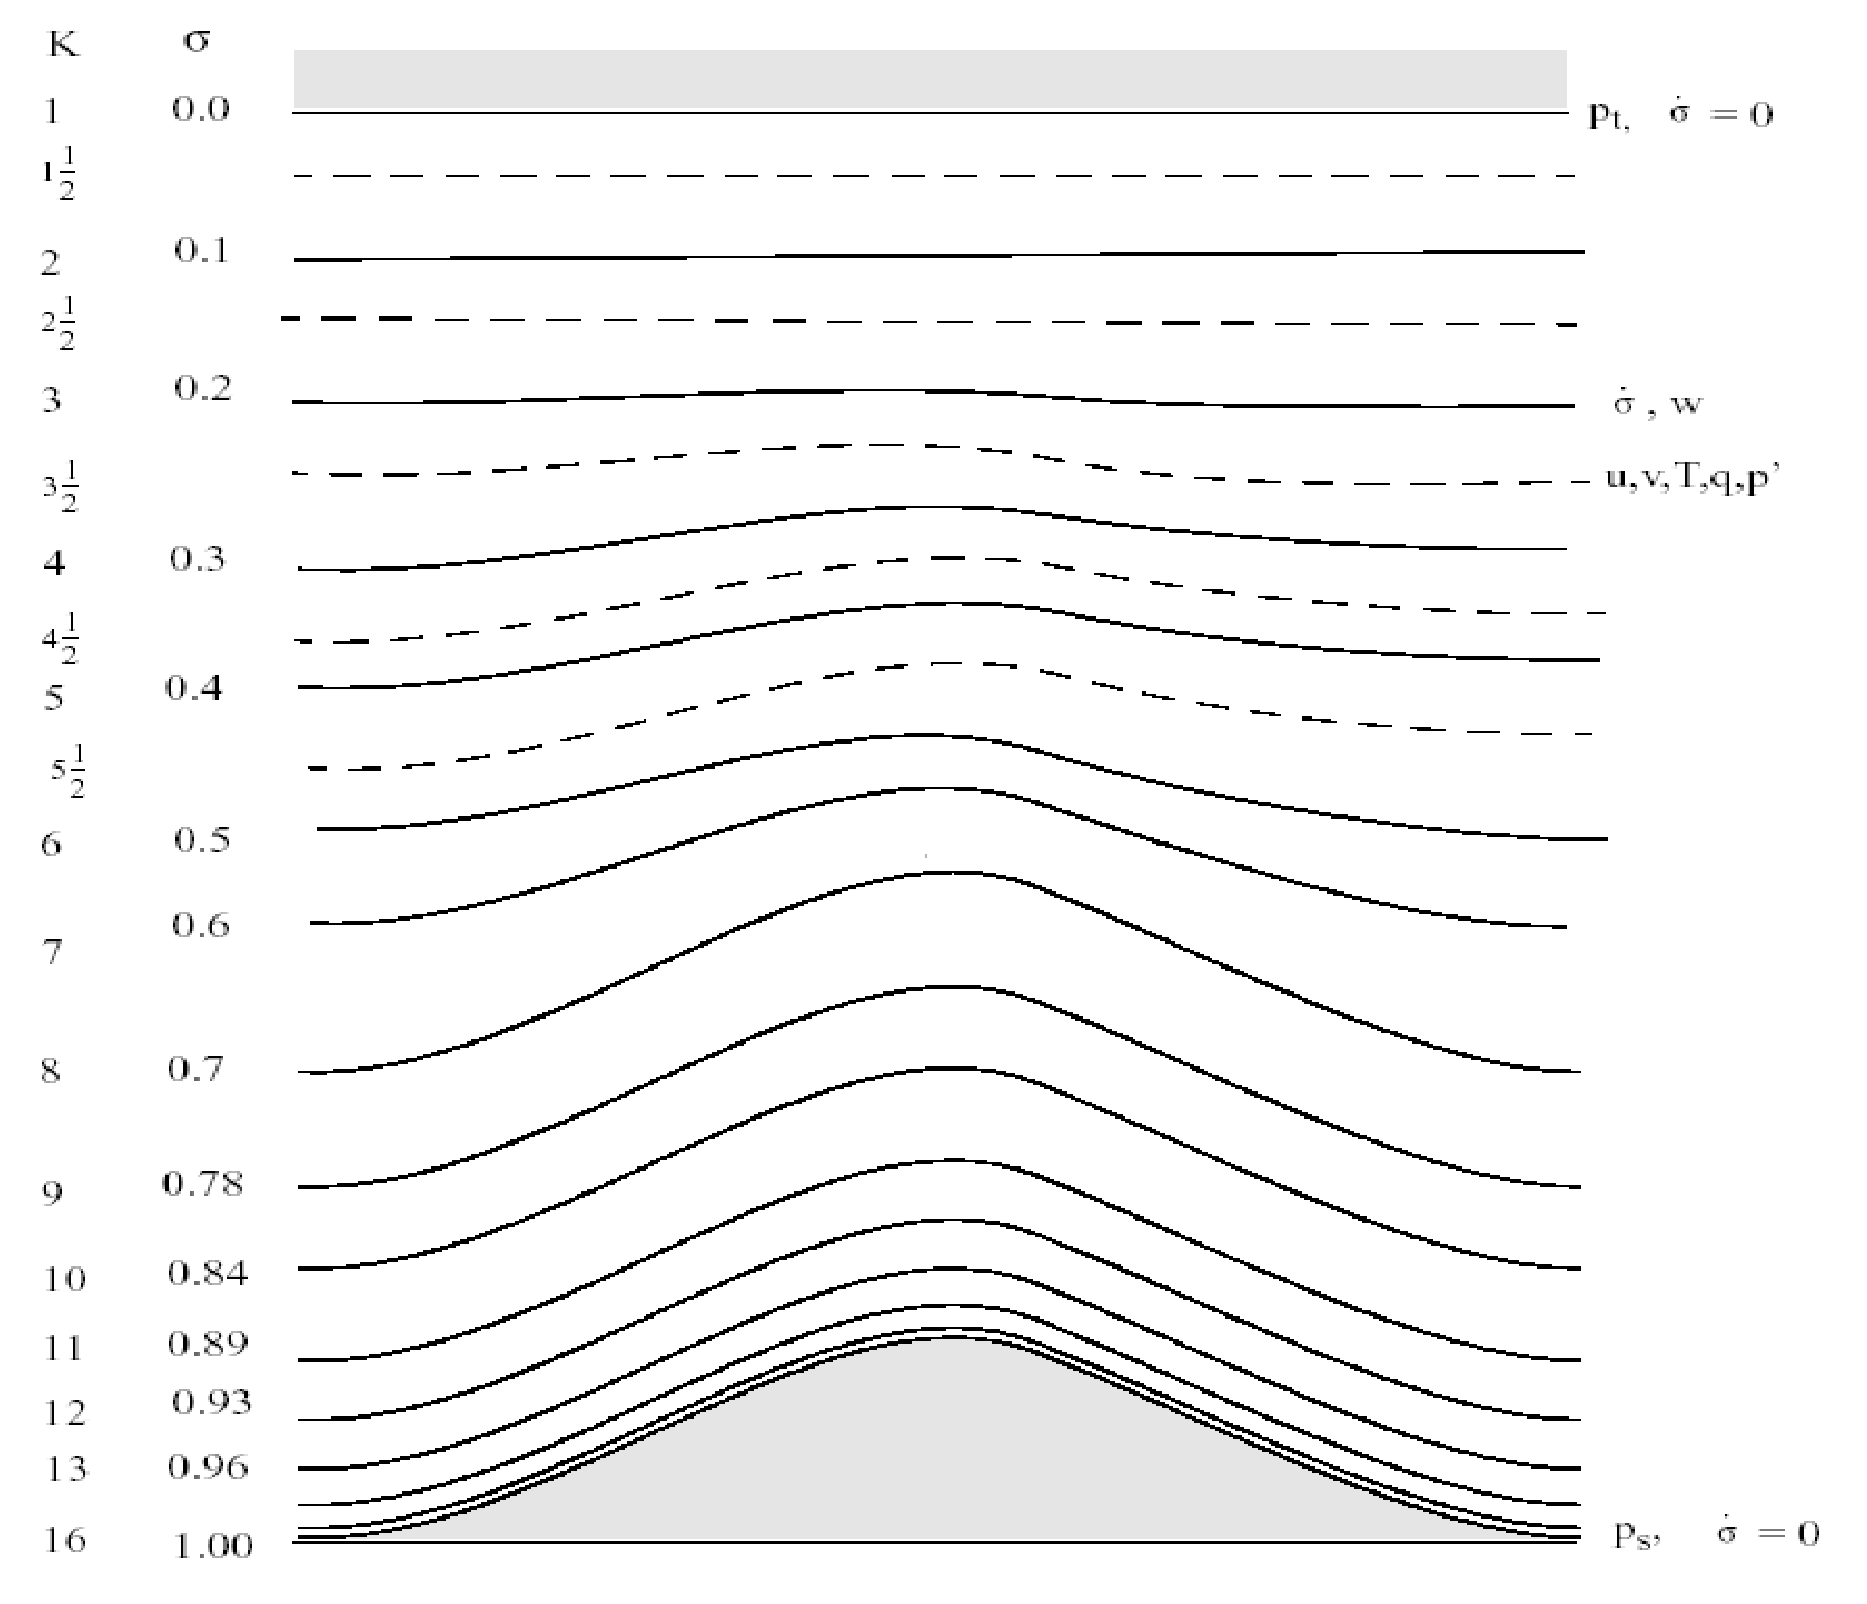
\includegraphics{sigma_levels.eps}}
\caption{Schematic representation of the vertical structure of the model.
This example is for 16 vertical layers. Dashed lines denote half-sigma levels,
solid lines denote full-sigma levels. (Adapted from the PSU/NCAR Mesoscale
Modeling System Tutorial Class Notes and User's Guide.)}
\label{sigma_levels}
\end{figure}

It is useful to first introduce the model's grid configuration. The modeling
system usually gets and analyzes its data on pressure surfaces, but these have
to be interpolated to the model's vertical coordinate before input to the model.
The vertical coordinate is terrain-following (Figure~\ref{sigma_levels}) meaning
that the lower grid levels follow the terrain while the upper surface is
flatter. Intermediate levels progressively flatten as the pressure decreases
toward the top of the model. 

The Hydrostatic solver uses A dimensionless $\sigma$ coordinate to
define the model levels where $p$ is the pressure, $p_t$ is a specified
constant top pressure, $p_s$ is the surface pressure.
\begin{eqnarray}
  \sigma = {(p - p_t) \over (p_s - p_t)}
\end{eqnarray}

where we can define:

\begin{eqnarray}
  p^*(x,y) = p_s(x,y) - p_t
\end{eqnarray}

For the Non-hydrostatic solver a similar dimensionless coordinate is used,
but it is defined entirely from the reference pressure. Given a reference
atmospheric profile:

\begin{eqnarray}
  p(x,y,z,t) = p_0(z) + p^\prime(x,y,z,t) \\
  T(x,y,z,t) = T_0(z) + T^\prime(x,y,z,t) \\
  \rho(x,y,z,t) = \rho_0(z) + \rho^\prime(x,y,z,t)
\end{eqnarray}

the vertical sigma coordinate is defined as:

\begin{eqnarray}
  \sigma = {(p_0 - p_t) \over (p_s - p_t)}
\end{eqnarray}

where $p_s$ is the surface pressure, $p_t$ is a specified constant top
pressure and $p_0$ is the reference pressure profile. The total pressure
at each grid point is thus given as:

\begin{eqnarray}
 p = p^*\sigma + p_t + p^\prime
\end{eqnarray}

with $p^*$ defined as in the hydrostatic solver.

It can be seen from the equation and Figure~\ref{sigma_levels} that $\sigma$ is
zero at the top and one at the surface, and each model level is defined by a
value of $\sigma$. The model vertical resolution is defined by a list of values
between zero and one that do not necessarily have to be evenly spaced. Commonly
the resolution in the boundary layer is much finer than above, and the number of
levels may vary upon the user demand.

\begin{figure}
\begin{center}
\resizebox{5.5in}{!}{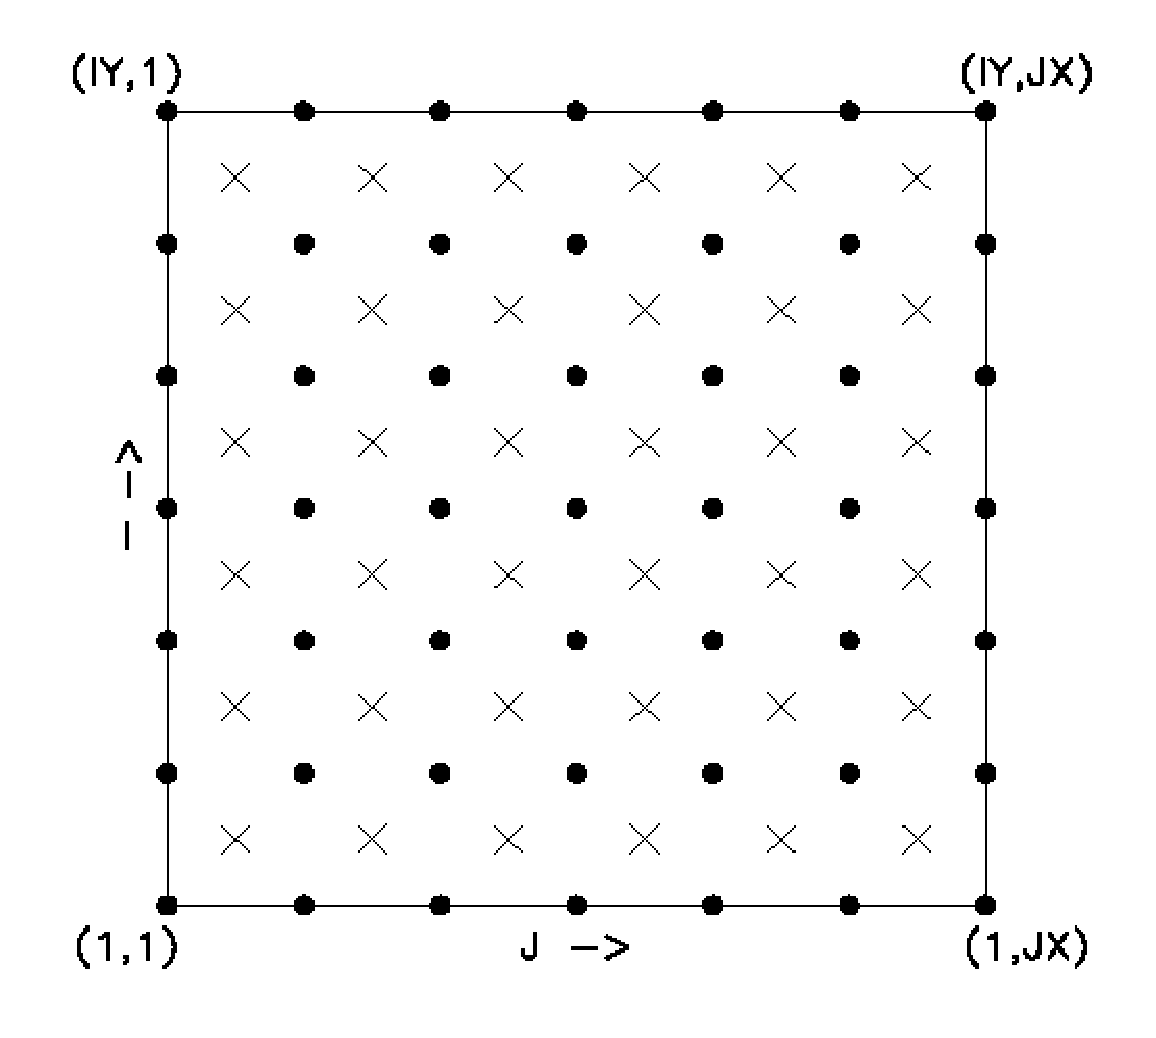
\includegraphics{grid2.eps}}
\caption{Schematic representation showing the horizontal Arakawa B-grid
staggering of the dot and cross grid points.}
\label{grid}
\end{center}
\end{figure}

The horizontal grid has an Arakawa-Lamb B-staggering of the velocity variables
with respect to the scalar variables. This is shown in Figure~\ref{grid} where
it can be seen that the scalars (T, q, p, etc) are defined at the center of the
grid box, while the eastward (u) and northward (v) velocity components are
collocated at the corners. The center points of grid squares will be referred to
as cross points, and the corner points are dot points.  Hence horizontal
velocity is defined at dot points. Data is input to the model, the preprocessors
do the necessary interpolation to assure consistency with the grid.

All the above variables are defined in the middle of each model vertical layer,
referred to as half-levels and represented by the dashed lines in
Figure~\ref{sigma_levels}. Vertical velocity is carried at the full levels
(solid lines). In defining the sigma levels it is the full levels that are
listed, including levels at $\sigma$ = 0 and 1. The number of model layers is
therefore always one less than the number of full sigma levels.

The finite differencing in the model is, of course, crucially dependent upon the
grid staggering wherever gradients or averaging are represented terms in the
equation.

\section{Map Projections and Map-Scale Factors}
The modeling system has a
choice of four map projections. Lambert Conformal is suitable for mid-latitudes,
Polar Stereographic for high latitudes, Normal Mercator for low latitudes, and
Rotated Mercator for extra choice. The $x$ and $y$ directions in the model do
not correspond to west-east and north-south except for the Normal Mercator
projection, and therefore the observed wind generally has to be rotated to the
model grid, and the model $u$ and $v$ components need to be rotated before
comparison with observations. These transformations are accounted for in the
model pre-processors that provide data on the model grid (Please note that
model output of u and v components, raw or postprocessed, should be rotated to a
lat/lon grid before comparing to observations).  The map scale factor, $m$, is
defined by:

\begin{equation}
  m = \frac{model\_grid\_distance}{real\_earth\_distance}
\end{equation}

\noindent \\ and its value is usually close to one, varying with latitude. The
projections in the model preserve the shape of small areas, so that $dx=dy$
everywhere, but the grid length varies across the domain to allow a
representation of a spherical surface on a plane surface. Map-scale factors need
to be accounted for in the model equations wherever horizontal gradients are
used.


%%
%%   This file is part of ICTP RegCM.
%%
%%   ICTP RegCM is free software: you can redistribute it and/or modify
%%   it under the terms of the GNU General Public License as published by
%%   the Free Software Foundation, either version 3 of the License, or
%%   (at your option) any later version.
%%
%%   ICTP RegCM is distributed in the hope that it will be useful,
%%   but WITHOUT ANY WARRANTY; without even the implied warranty of
%%   MERCHANTABILITY or FITNESS FOR A PARTICULAR PURPOSE.  See the
%%   GNU General Public License for more details.
%%
%%   You should have received a copy of the GNU General Public License
%%   along with ICTP RegCM.  If not, see <http://www.gnu.org/licenses/>.
%%

\newpage

\chapter{Model Equations}

The RegCM model solves a set of primitive dynamical equations describing
the atmospheric motion, with parametrizations for physical processes as per:

\begin{itemize}
	\item Radiation (Short Wave and Long Wave)
	\item Convection
	\item Turbolent Diffusion
	\item Moist (Clouds and Precipitation)
	\item Fluxes exchange with surface (Soil model and Ocean fluxes)
	\item Tracer transport and chemistry (Aerosols and full chemistry)
\end{itemize}

The dynamical equations are discretized using finite differences technique
on a three dimensional computation grid with fixed horizontal resolution
and terrain following vertical coordinate.

\section{Dynamics}
The model has two dynamical cores:

\begin{itemize}
\item Hydrostatic equation solver
\item Non-hydrostatic equation solver
\end{itemize}

The primitive equations for the two solvers are different and have different
prognostic variables used to identify the atmospheric state.

\subsection{Hydrostatic dynamical core}
The hydrostatic model dynamic equations and numerical discretization are
described by \cite{Grell_94}.

\subsubsection{Horizontal Momentum Equations}

\begin{gather}
\label{hydro1}
	\frac{\partial{p^{\ast}u}}{\partial{t}} =
	-m^2 \left[ \frac{\partial{p^{\ast}uu/m}}{\partial{x}} + 
		\frac{\partial{p^{\ast}vu/m}}{\partial{y}} \right] -
		\frac{\partial{p^{\ast}u \dot{\sigma}}}{\partial{\sigma}}
	    \\ \nonumber
	    -mp^{\ast} \left[ \frac{\sigma}{\rho}
			\frac{\partial{p^{\ast}}}{\partial{x}} +
			\frac{\partial{\phi}}{\partial{x}} \right] +
	p^{\ast}fv + F_Hu + F_Vu \\
\label{hydro2}
	\frac{\partial{p^{\ast}v}}{\partial{t}} = 
	-m^2 \left[ \frac{\partial{p^{\ast}uv/m}}{\partial{x}} +
		\frac{\partial{p^{\ast}vv/m}}{\partial{y}} \right] -
		\frac{\partial{p^{\ast}v\dot{\sigma}}}{\partial{\sigma}}
	   \\ \nonumber
	   -mp^{\ast} \left[ \frac{\sigma}{\rho}
	   		\frac{\partial{p^{\ast}}}{\partial{y}} +
			\frac{\partial{\phi}}{\partial{y}} \right]
	+ p^{\ast}fu + F_Hv + F_Vv
\end{gather}

where $u$ and $v$ are the eastward and northward components of
velocity, $\phi$ is geopotential height, $f$ is the coriolis parameter,
$m$ is the map scale factor for the chosen projection, and $F_H$ and $F_V$
represent the effects of horizontal and vertical diffusion, and
$p^{\ast} = p_s-p_t$, i.e. the difference between surface and model top
pressure.  \\

In the equation \ref{hydro1} - \ref{hydro2}, $\dot{\sigma}$ is the total
derivative of the vertical coordinate $\sigma$ over time $t$:

\begin{equation}
\dot{\sigma} = {d\sigma \over dt}
\end{equation}

Moreover, given $T_v$ as the virtual temperature:

\begin{equation}
T_v = T \left( 1 + 0.608 Q_v \right)
\end{equation}

then

\begin{equation}
\frac{\sigma}{\rho} = \frac{RT_v}{(p^{\ast} + p_t/\sigma)}
\end{equation}

with $R$ the gas constant for dry air

\subsubsection{Continuity and Sigmadot $({\bf \dot{\sigma}})$ Equations}

The surface pressure is computed from the continuity equation:

\begin{eqnarray} \label{eq:continuity}
\frac{\partial{p^{\ast}}}{\partial{t}} = 
	-m^2 \left[ \frac{\partial{p^{\ast}u/m}}{\partial{x}} +
		    \frac{\partial{p^{\ast}v/m}}{\partial{y}} \right] -
	\frac{\partial{p^{\ast}\dot{\sigma}}}{\partial{\sigma}}
\end{eqnarray}

The vertical integral of Equation~\ref{eq:continuity} is used to
compute the temporal variation of the surface pressure in the model,

\begin{eqnarray}
\label{intform}
	\frac{\partial{p^{\ast}}}{\partial{t}} = -m^2 \int_{0}^{1}
	{\left[ \frac{\partial{p^{\ast}u/m}}{\partial{x}} + 
		\frac{\partial{p^{\ast}v/m}}{\partial{y}} \right] d\sigma}
\end{eqnarray}

The surface pressure tendency from \ref{intform} is then used with the
the vertical integral of \ref{eq:continuity} to compute the vertical
velocity in sigma coordinates $(\dot{\sigma})$ at each
level in the model:

\begin{eqnarray}
	\dot{\sigma} = - \frac{1}{p^{\ast}} \int_{0}^{\sigma}{
		\left[ \frac{\partial{p^{\ast}}}{\partial{t}} +
		m^2 \left(\frac{\partial{p^{\ast}u/m}}{\partial{x}} +
		                 \frac{\partial{p^{\ast}v/m}}{\partial{y}}
	 \right) \right] d\sigma^\prime}
\end{eqnarray}

where $\sigma^\prime$ is a dummy variable of integration and
$\dot{\sigma}(\sigma=0)=0$.

\subsubsection{Thermodynamic Equation and Equation for Omega ${\bf (\omega)}$}

The thermodynamic equation is

\begin{eqnarray}
\frac{\partial{p^{\ast}T}}{\partial{t}} = 
-m^2 \left[ \frac{\partial{p^{\ast}uT/m}}{\partial{x}} +
	    \frac{\partial{p^{\ast}vT/m}}{\partial{y}} \right] -
	    \frac{\partial{p^{\ast}T\dot{\sigma}}}{\partial{\sigma}} +
	    \nonumber \\
	\frac{RT_v\omega}{c_{p}(\sigma + p_t/p_{\ast})} +
	\frac{p^{\ast}Q}{c_{p}} + F_HT + F_VT
\end{eqnarray}

where, given $c_{pd}$ the heat capacity of dry air and $q_v$ the water vapor
mixing ratio:

\begin{equation}
c_{p} = c_{pd} \left( 1 + 0.8q_v \right)
\end{equation}

$c_p$ is the specific heat for moist air at constant pressure, $Q$ is the
diabatic heating, $F_HT$ represents the effect of horizontal diffusion,
$F_VT$ represents the effect of vertical mixing and dry convective adjustment,
and $\omega$ is

\begin{equation}
\omega = p^{\ast} \dot{\sigma} + \sigma \frac{dp^{\ast}}{dt}
\end{equation}

where:
  
\begin{eqnarray}
\frac{dp^{\ast}}{dt} =
   \frac{\partial{p^{\ast}}}{\partial{t}} + m
   \left[ u \frac{\partial{p^{\ast}}}{\partial{x}} +
          v \frac{\partial{p^{\ast}}}{\partial{y}} \right]
\end{eqnarray}

\subsubsection{Hydrostatic Equation}

The hydrostatic equation is used to compute the geopotential heights from
the virtual temperature $T_v$,

\begin{eqnarray}
\frac{\partial{\phi}}{\partial{\ln(\sigma + p_t / p^{\ast})}} =
-RT_v \left[ 1 + \frac{\sum{q_x}}{1 + q_v} \right]^{-1}
\end{eqnarray}

where $T_v = T(1 + 0.608q_v)$, $q_v$, is the water vapor mixing ratio, and
$q_x$ are the mixing ratios of all condensed water species.

\subsubsection{Split-explicit timestep for fast waves removal}


\newpage

\subsection{Non-hydrostatic dynamical core}
The non-hydrostatic model dynamic equations and numerical discretization are
described by \cite{Grell_94}.

\subsubsection{Model Equations}

Being $p^{\ast}$ constant in time, in the non-hydrostatic the continuity
equation no longer applies, thus the $DIV$ term appear in the equations
\ref{non-hydro-eq-first}-\ref{non-hydro-eq-last}:

\begin{gather}
\label{non-hydro-eq-first}
\frac{\partial{p^{\ast} u}}{\partial{t}} = -m^2 \left[ 
	\frac{\partial{p^{\ast} uu/m}}{\partial{x}} + 
\frac{\partial{p^{\ast} vu/m}}{\partial{y}}\right] -
	\frac{\partial{p^{\ast} u \dot{\sigma}}}{\partial{\sigma}} + 
	uDIV \\ \nonumber
	-\frac{mp^{\ast}}{\rho} \left[
		\frac{\partial{p^\prime}}{\partial{x}} -
		\frac{\sigma}{p^{\ast}}
		\frac{\partial{p^{\ast}}}{\partial{x}}
	        \frac{\partial{p^\prime}}{\partial{\sigma}}\right] +
	p^{\ast}fv - p^{\ast} ew \cos\theta + D_u  \\
\frac{\partial{p^{\ast} v}}{\partial{t}}= -m^2 \left[ 
	\frac{\partial{p^{\ast} uv/m}}{\partial{x}} + 
	\frac{\partial{p^{\ast} vv/m}}{\partial{y}}\right] -
	\frac{\partial{p^{\ast} v \dot{\sigma}}}{\partial{\sigma}}+ 
	vDIV \\ \nonumber
	-\frac{mp^{\ast}}{\rho} \left[
		\frac{\partial{p^\prime}}{\partial{y}} -
		\frac{\sigma}{p^{\ast}}
		\frac{\partial{p^{\ast}}}{\partial{y}}
		\frac{\partial{p^\prime}}{\partial{\sigma}} \right] -
	p^{\ast}fu + p^{\ast} ew \sin\theta + D_v \\
\frac{\partial{p^{\ast} w}}{\partial{t}} = -m^2 \left[ 
	\frac{\partial{p^{\ast} uw/m}}{\partial{x}} + 
	\frac{\partial{p^{\ast} vw/m}}{\partial{y}}\right] -
	\frac{\partial{p^{\ast} w \dot{\sigma}}}{\partial{\sigma}} + 
	wDIV \\ \nonumber
	+ p^{\ast}g\frac{\rho_0}\rho{}\left[
		\frac{1}{p^{\ast}}
		\frac{\partial{p^\prime}}{\partial{\sigma}} +
		\frac{T^{\prime}_{v}}{T} -
		\frac{T_0 p^\prime}{Tp_0} \right]
	-p^{\ast} g \left[\left(q_c+q_r\right)\right] \\ \nonumber
	+ p^{\ast} e \left( u\cos\theta - v\sin\theta \right) + D_w \\
\frac{\partial{p^{\ast} p^\prime}}{\partial{t}} = -m^2 \left[ 
	\frac{\partial{p^{\ast} up^\prime/m}}{\partial{x}} + 
	\frac{\partial{p^{\ast} vp^\prime/m}}{\partial{y}}\right] -
	\frac{\partial{p^{\ast} p^\prime \dot{\sigma}}}{\partial{\sigma}} + 
	p^{\prime}DIV \\ \nonumber
	- m^2 p^{\ast} \gamma p \left[
		\frac{\partial{u/m}}{\partial{x}} -
		\frac{\sigma}{mp^{\ast}}
		\frac{\partial{p^{\ast}}}{\partial{x}}
		\frac{\partial{u}}{\partial{\sigma}} + 
		\frac{\partial{v/m}}{\partial{y}} -
		\frac{\sigma}{mp^{\ast}}
		\frac{\partial{p^{\ast}}}{\partial{y}}
		\frac{\partial{v}}{\partial{\sigma}} \right] \\ \nonumber
	+ \rho_0 g \gamma p \frac{\partial{w}}{\partial{\sigma}} +
	p^{\ast} \rho_0 gw \\
\label{non-hydro-eq-last}
\frac{\partial{p^{\ast} T}}{\partial{t}} = -m^2 \left[
	\frac{\partial{p^{\ast} uT/m}}{\partial{x}} +
	\frac{\partial{p^{\ast} vT/m}}{\partial{y}} \right] -
	\frac{\partial{p^{\ast} T \dot{\sigma}}}{\partial{\sigma}} +
	TDIV \\ \nonumber
	+\frac{1}{\rho c_p}\left[p^{\ast}\frac{Dp^{\prime}}{Dt} -
	\rho_0gp^{\ast}w -D_{p^\prime}\right] +
	p^{\ast}\frac{\dot{Q}}{c_p} +D_T
\end{gather}

where:

\begin{eqnarray}
	DIV = m^2 \left[ \frac{\partial{p^{\ast}u/m}}{\partial{x}} +
		\frac{\partial{p^{\ast} v/m}}{\partial{y}} \right] +
		\frac{\partial{p^{\ast} \dot{\sigma}}}{\partial{\sigma}} \\
  \dot{\sigma} = - \frac{\rho_0g}{p^{\ast}}w -
                   \frac{m\sigma}{p^{\ast}}
		   \frac{\partial{p^{\ast}}}{\partial{x}}u -
		   \frac{m\sigma}{p^{\ast}}
		   \frac{\partial{p^{\ast}}}{\partial{y}} v \\
   \tan \theta = - \cos \phi \frac{\partial{\lambda}/ \partial{y}}
				  {\partial{\phi}/ \partial{x}} \\ \nonumber
				 \phi = latitude \\ \nonumber
				 \lambda = longitude \\
   \gamma = c_p / c_v
\end{eqnarray}

\subsubsection{Sound Waves}

For the non-hydrostatic equations, the acoustic wave terms are separated
from the slow varying terms and handled with a shorter time steps. The reduced
equations contain only interactions between momentum and pressure:

\begin{gather}
\frac{\partial{u}}{\partial{t}} + \frac{m}{\rho} \left[
		\frac{\partial{p^\prime}}{\partial{x}} -
		\frac{\sigma}{p^{\ast}}
		\frac{\partial{p^\ast}}{\partial{x}}
		\frac{\partial{p^\prime}}{\partial{\sigma}} \right] = S_u \\
\frac{\partial{v}}{\partial{t}} + \frac{m}{\rho} \left[
		\frac{\partial{p^\prime}}{\partial{y}} -
		\frac{\sigma}{p^{\ast}}
		\frac{\partial{p^\ast}}{\partial{y}}
		\frac{\partial{p^\prime}}{\partial{\sigma}} \right] = S_v \\
\frac{\partial{w}}{\partial{t}} - \frac{\rho_0}{\rho} 
	\frac{g}{p^\ast}\frac{\partial{p^\prime}}{\partial{\sigma}} +
	\frac{g}{\gamma} \frac{p^\prime}{p} = S_w \\
\frac{\partial{p^\prime}}{\partial{t}} + m^2 \gamma p \left[
	  \frac{\partial{u/m}}{\partial{x}} -
	  \frac{\sigma}{mp^\ast}
	  \frac{\partial{p^\ast}}{\partial{x}}
	  \frac{\partial{u}}{\partial{\sigma}} +
	  \frac{\partial{v/m}}{\partial{y}} -
	  \frac{\sigma}{mp^\ast}
	  \frac{\partial{p^\ast}}{\partial{y}}
	  \frac{\partial{v}}{\partial{\sigma}} \right] -
	  \frac{\rho_0 g \gamma p}{p^\ast}
	  \frac{\partial{w}}{\partial{\sigma}} - \rho_0 gw = S_{p^\prime}
\end{gather}

with $\gamma$ the ratio of the specific heats at constant pressure and volume.
During the small time-steps, the $S_x$ terms are kept constant (they contain
advection, diffusion, buoyancy and coriolis tendencies), and following the
semi-implicit scheme in \cite{Klemp_1978} we solve the above by recursion.
The step only depends on the horizontal grid size.

\section{Physics parametrizations} \label{sec:physics}

\subsection{Radiation Scheme}

\noindent RegCM4 uses the radiation scheme of
the NCAR CCM3, which is described in \cite{Kiehl_96}.  Briefly, the solar
component, which accounts for the effect of ${\rm O_3}$, ${\rm H_2O}$, ${\rm
CO_2}$, and ${\rm O_2}$, follows the $\delta$-Eddington approximation of
\cite{Kiehl_96}.  It includes 18 spectral intervals from 0.2 to 5 $\mu {\rm m}$.
The cloud scattering and absorption parameterization follow that of
\cite{Slingo_89}, whereby the optical properties of the cloud droplets
(extinction optical depth, single scattering albedo, and asymmetry parameter)
are expressed in terms of the cloud liquid water content and an effective
droplet radius.  When cumulus clouds are formed, the gridpoint fractional cloud
cover is such that the total cover for the column extending from the
model-computed cloud-base level to the cloud-top level (calculated assuming
random overlap) is a function of horizontal gridpoint spacing.  The thickness of
the cloud layer is assumed to be equal to that of the model layer, and a
different cloud water content is specified for middle and low clouds.

\subsection{Land Surface Models}

\noindent {\bf BATS (default):} BATS is a surface package designed to describe
the role of vegetation and interactive soil moisture in modifying the
surface-atmosphere exchanges of momentum, energy, and water vapor (see
\cite{Dickinson_93} for details).  The model has a vegetation layer, a snow
layer, a surface soil layer, 10~cm thick, or root zone layer, 1-2~m thick, and a
third deep soil layer 3~m thick.  Prognostic equations are solved for the soil
layer temperatures using a generalization of the force-restore method of
\cite{Deardoff_78}.  The temperature of the canopy and canopy foilage is
calculated diagnostically via an energy balance formulation including sensible,
radiative, and latent heat fluxes.

The soil hydrology calculations include predictive equations for the water
content of the soil layers.  These equations account for precipitation,
snowmelt, canopy foiliage drip, evapotranspiration, surface runoff, infiltration
below the root zone, and diffusive exchange of water between soil layers.  The
soil water movement formulation is obtained from a fit to results from a
high-resolution soil model \cite{Dickinson_84} and the surface runoff rates are
expressed as functions of the precipitation rates and the degree of soil water
saturation.  Snow depth is prognostically calculated from snowfall, snowmelt,
and sublimation.  Precipitation is assumed to fall in the form of snow if the
temperature of the lowest model level is below 271~K.

Sensible heat, water vapor, and momentum fluxes at the surface are calculated
using a standard surface drag coefficient formulation based on surface-layer
similarity theory.  The drag coefficient depends on the surface roughness length
and on the atmospheric stability in the surface layer.  The surface
evapotranspiration rates depend on the availability of soil water.  \ac{BATS}
has 20 vegetation types (Table~\ref{landuse};  soil textures ranging from coarse
(sand), to intermediate (loam), to fine (clay);  and different soil colors
(light to dark) for the soil albedo calculations.  These are described in
\cite{Dickinson_86}. 

In the latest release version, additional modifications have been made to
\ac{BATS}in order to account for the subgrid variability of topography and
landcover using a mosaic-type approach \citep{Giorgi03b}.  Thismodification
adopts a regular fine-scale surface subgrid for eachcoarse model grid cell.
Meteorological variables are disaggregatedfrom the coarse grid to the fine
grid based on the elevationdifferences.  The \ac{BATS} calculations are then
performed separatelyfor each subgrid cell, and surface fluxes are reaggregated
onto thecoarse grid cell for input to the atmospheric model.
This parameterization showed a marked improvement in the representation ofthe
surface hydrological cycle in mountainous regions \citep{Giorgi03b}.
As a first augmentation, in \ac{RegCM4} two new land use types were added to
\ac{BATS} to represent urban and sub-urban environments. Urban development not
only modifies the surface albedo and alters the surface energy balance, but
also creates impervious surfaces with large effects on runoff and
evapotranspiration.
These effects can be described by modifying relevant properties of the land
surface types in the BATS package, such as maximum vegetation cover, roughness
length, albedo, and soil characteristics. For this purpose, we implemented the
parameters proposed in Table 1 of \cite{Kueppers_08}.

\noindent {\bf CLM (optional):} The Community Land Model (CLM; \cite{Oleson_08})
is the land surface model developed by the National Center of Atmospheric
Research (NCAR) as part of the Community Climate System Model (CCSM), described
in detail in \cite{Collins_06}.  CLM version 3.5 was coupled to RegCM for a more
detailed land surface description option.  CLM contains five possible snow
layers with an additional representation of trace snow and ten unevenly spaced
soil layers with explicit solutions of temperature, liquid water and ice water
in each layer.  To account for land surface complexity within a climate model
grid cell, CLM uses a tile or “mosaic” approach to capture surface
heterogeneity.  Each CLM gridcell contains up to four different land cover types
(glacier, wetland, lake, and vegetated), where the vegetated fraction can be
further divided into 17 different plant functional types.  Hydrological and
energy balance equations are solved for each land cover type and aggregated back
to the gridcell level.  A detailed discussion of CLM version 3 implemented in
RegCM3 and comparative analysis of land surface parameterization options is
presented in \cite{Steiner_09}.  Since CLM was developed for the global scale,
several input files and processes were modified to make it more appropriate for
regional simulations, including (1) the use of high resolution input data, (2)
soil moisture initialization, and (3) and an improved treatment of grid cells
along coastlines.  For the model input data, CLM requires several time-invariant
surface input parameters:  soil color, soil texture, percent cover of each land
surface type, leaf and stem area indices, maximum saturation fraction, and land
fraction \citep{Lawrence_07}.  Table~\ref{clm} shows the resolution for each
input parameter used at the regional scale in RegCM-CLM compared to resolutions
typically used for global simulations.  The resolution of surface input
parameters was increased for several parameters to capture surface heterogeneity
when interpolating to the regional climate grid.  Similar to \cite{Lawrence_07},
the number of soil colors was extended from 8 to 20 classes to resolve regional
variations.  The second modification was to update the soil moisture
initialization based on a climatological soil moisture average
\citep{Giorgi_89b} over the use of constant soil moisture content throughout the
grid generally used for global CLM.  By using a climatological average for soil
moisture, model spin-up time is reduced with regards to deeper soil layers.  The
third modification to the CLM is the inclusion of a mosaic approach for
gridcells that contain both land and ocean surface types.  With this approach, a
weighted average of necessary surface variables was calculated for land/ocean
gridcells using the land fraction input dataset.  This method provides a better
representation of coastlines using the high-resolution land fraction data
described in Table~\ref{clm}.  For a more detailed description of CLM physics
parameterizations see \cite{Oleson_04}.

\begin{table}
\centering
\caption{Land Cover/Vegetation classes}
\label{VegTypes}
\begin{tabular}{rl}
\hline
\hline
1.&Crop/mixed farming\\
2.&Short grass\\
3.&Evergreen needleleaf tree\\
4.&Deciduous needleleaf tree\\
5.&Deciduous broadleaf tree\\
6.&Evergreen broadleaf tree\\
7.&Tall grass\\
8.&Desert\\
9.&Tundra\\
10.&Irrigated Crop\\
11.&Semi-desert\\
12.&Ice cap/glacier\\
13.&Bog or marsh\\
14.&Inland water\\
15.&Ocean\\
16.&Evergreen shrub\\
17.&Deciduous shrub\\
18.&Mixed Woodland\\
19.&Forest/Field mosaic \\
20.&Water and Land mixture \\
\hline
\hline
\end{tabular}
\end{table}

\newpage

\begin{landscape}
\begin{table}
\centering
\caption{BATS vegetation/land-cover}
\label{landuse}
{\small
\begin{tabular}{lcccccccccccccccccccc}
\hline
\hline
\multicolumn{1}{c}{Parameter}&\multicolumn{20}{c}{Land Cover/Vegetation Type}\\
&1&2&3&4&5&6&7&8&9&10&11&12&13&14&15&16&17&18&19&20 \\ \hline Max fractional \\
vegetation
cover&0.85&0.80&0.80&0.80&0.80&0.90&0.80&0.00&0.60&0.80&0.35&0.00&0.80&0.00&0.00&0.80&0.80&0.80&0.80&0.80
\\ Difference between max\\ fractional vegetation \\ cover and cover at 269
K&0.6&0.1&0.1&0.3&0.5&0.3&0.0&0.2&0.6&0.1&0.0&0.4&0.0&0.0&0.2&0.3&0.2&0.4&0.4 \\
Roughness length (m)
&0.08&0.05&1.00&1.00&0.80&2.00&0.10&0.05&0.04&0.06&0.10&0.01&0.03&0.0004&0.0004&0.10&0.10&0.80&0.3&0.3
\\ Displacement height (m)
&0.0&0.0&9.0&9.0&0.0&18.0&0.0&0.0&0.0&0.0&0.0&0.0&0.0&0.0&0.0&0.0&0.0&0.0&0.0&0.0
\\ Min stomatal \\ resistence (s/m)  &45 &60 &80 &80 &120 &60 &60 &200 &80 &45
&150 &200 &45 &200 &200 &80 &120 &100&120&120  \\ Max Leaf Area Index
&6   &2   &6   &6   &6   &6   &6   &0   &6   &6   &6   &0   &6   &0   &0   &6
&6   &6 &6 &6    \\ Min Leaf Area Index            &0.5 &0.5 &5   &1   &1   &5
&0.5 &0   &0.5 &0.5 &0.5 &0   &0.5 &0   &0   &5   &1   &3  &0.5 &0.5   \\ Stem
(dead matter \\ area
index)&0.5&4.0&2.0&2.0&2.0&2.0&2.0&0.5&0.5&2.0&2.0&2.0&2.0&2.0&2.0&2.0&2.0&2.0&2.0&2.0
\\ Inverse square root of \\ leaf dimension
(m$^{-1/2}$)&10&5&5&5&5&5&5&5&5&5&5&5&5&5&5&5&5&5&5&5\\ Light sensitivity \\
factor (m$^2$
W$^{-1}$)&0.02&0.02&0.06&0.06&0.06&0.06&0.02&0.02&0.02&0.02&0.02&0.02&0.02&0.02&0.02&0.02&0.02&0.06&0.02&0.02
\\ Upper soil layer \\ depth (mm)     &100 &100 &100 &100 &100 &100 &100 &100
&100 &100 &100 &100 &100 &100 &100 &100 &100 &100 &100 &100  \\ Root zone soil\\
layer depth (mm) &1000 &1000 &1500 &1500 &2000 &1500 &1000 &1000 &1000 &1000
&1000 &1000 &1000 &1000 &1000 &1000 &1000 &2000 &2000 &2000  \\ Depth of total\\
soil (mm) &3000 &3000 &3000 &3000 &3000 &3000 &3000 &3000 &3000 &3000 &3000
&3000 &3000 &3000 &3000 &3000 &3000 &3000 &3000 &3000  \\ Soil texture type
&6   &6   &6   &6   &7   &8   &6   &3   &6   &6   &5   &12   &6   &6   &6   &6
&5   &6 &6 &0    \\ Soil color type    &5   &3   &4   &4   &4   &4   &4   &1
&3   &3   &2   &1   &5   &5   &5   &4   &3   &4 &4 &0    \\ Vegetation albedo
for \\ wavelengths $<$ 0.7 $\mu$ m
&0.10&0.10&0.05&0.05&0.08&0.04&0.08&0.20&0.10&0.08&0.17&0.80&0.06&0.07&0.07&0.05&0.08&0.06
&0.06 &0.06 \\ Vegetation albedo for \\ wavelengths $>$ 0.7 $\mu$ m
&0.30&0.30&0.23&0.23&0.28&0.20&0.30&0.40&0.30&0.28&0.34&0.60&0.18&0.20&0.20&0.23&0.28&0.24&0.18&0.18 \\
\hline
\hline
\end{tabular}
}
\end{table}
\end{landscape}
\newpage

\begin{table}
\centering
\caption{Resolution for CLM input parameters}
\begin{tabular}{ l  c c c   }
\hline
\hline
Input data & Grid Spacing & Lon range & Lat range \\
\hline
Glacier      & $0.05^{\circ}$ x $0.05^{\circ}$ & $\pm 179.975$ & $\pm 89.975$ \\Lake         & $0.05^{\circ}$ x $0.05^{\circ}$ & $\pm 179.975$ & $\pm 89.975$ \\
Wetland      & $0.05^{\circ}$ x $0.05^{\circ}$ & $\pm 179.975$ & $\pm 89.975$ \\
Land fraction& $0.05^{\circ}$ x $0.05^{\circ}$ & $\pm 179.975$ & $\pm 89.975$ \\
LAI/SAI      & $0.5^{\circ}$ x $0.5^{\circ}$   & $\pm 179.75$  & $\pm 89.75$  \\
PFT          & $0.5^{\circ}$ x $0.5^{\circ}$   & $\pm 179.75$  & $\pm 89.75$  \\
Soil color   & $0.05^{\circ}$ x $0.05^{\circ}$ & $\pm 179.975$ & $\pm 89.975$ \\
Soil texture & $0.05^{\circ}$ x $0.05^{\circ}$ & $\pm 179.975$ & $\pm 89.975$ \\
Max. sat. area  & $0.5^{\circ}$ x $0.5^{\circ}$ & $\pm 179.75$ & $\pm 89.75$  \\
\hline
\hline
\label{clm}
\end{tabular}
\end{table}

\subsection{Planetary Boundary Layer Scheme}
\subsubsection{Holtslag PBL}

The Holtslag planetary boundary layer scheme, developed by \cite{Holtslag_90},
is based on a nonlocal diffusion concept that takes into account
countergradient fluxes resulting from large-scale eddies in an unstable,
well-mixed atmosphere.  The vertical eddy flux within the PBL is given by

\begin{eqnarray}
F_c = -K_c \left( {\partial{C} \over \partial{z}} - \gamma_c \right)
\end{eqnarray}

where $\gamma_c$ is a ``countergradient'' transport term describing
nonlocal transport due to dry deep convection.  The eddy diffusivity is given by
the nonlocal formulation

\begin{eqnarray}
K_c = kw_tz \left( 1- {z \over h} \right)^2
\end{eqnarray}

where $k$ is the von Karman constant; $w_t$ is a turbulent convective
velocity that depends on the friction velocity, height, and the Monin--Obhukov
length;  and $h$ is the PBL height.

The countergradient term for temperature and water vapor is given by

\begin{eqnarray}
\label{eq:countergradient}
\gamma_c = C { {\phi_c}^0 \over w_t h}
\end{eqnarray}

where C is a constant equal to 8.5, and ${\phi_c}^0$ is the surface
temperature or water vapor flux. Equation~\ref{eq:countergradient} is applied
between the top of the PBL and the top of the surface layer, which is assumed to
be equal to $0.1h$. Outside this region and for momentum, $\gamma_c$ is assumed
to be equal to 0.  

For the calculation of the eddy diffusivity and countergradient terms, the PBL
height is diagnostically computed from

\begin{eqnarray}
  h = { {\rm {R_i}_{cr}} [u(h)^2 + v(h)^2] \over (g/\theta_s)[\theta_v(h)-\theta_s] }
\end{eqnarray}

where $u(h)$, $v(h)$, and $\theta_v$ are the wind components and the
virtual potential temperature at the PBL height, $g$ is gravity, ${\rm {R_i}_{cr}}$
is the critical bulk Richardson number, and $\theta_s$ is an appropriate
temperature of are near the surface.  Refer to \cite{Holtslag_90} and
\cite{Holtslag_93} for a more detailed description.

Compared to other schemes this formulation tends to produce relatively strong,
and often excessive, turbulent vertical transfer.
For example, after extensive testing, we found excessive vertical transfer
of moisture in the model resulting in low moisture amounts near the surface
and excessive moisture near the PBL top.

Therefore in order to ameliorate this problem, the countergradient term for
water vapor was removed in \ac{RegCM4}. Another problem of the Holtslag scheme
(at least in our implementation) is an excessive vertical transport of heat,
moisture and momentum in very stable conditions, such as during the winter in
northern hemisphere high latitude regions. For example we found that in such
conditions the scheme fails to simulate near surface temperature inversions.

This in turn leads to large warm winter biases (even > 10 degrees) over regions
such as Northern Siberia and Northern Canada. As an ad-hoc fix to address this
problem, in \ac{RegCM4} we implemented the following modification to the scheme:

\begin{itemize}
\item We first define “very stable” conditions within the Holtslag
parameterization as conditions in which the ratio of the height from the
surface over the Monin-Obhukov length is lower than 0.1.
\item When such conditions are found, we set to 0 the eddy diffusivity
and counter-gradient terms for all variables.
\end{itemize}

Preliminary tests showed that this modification reduces the warm bias in high
latitude winter conditions and allows the model to better capture surface
inversions. These modifications have thus been incorporated as default in the
\ac{RegCM4} code.

\subsubsection{The UW Turbulence Closure Model}

As an alternative to the Holtslag PBL, the University of Washington turbulence
closure model \citep{Grenier_01,Bretherton_04} has been coupled to RegCM.  The
development of this coupling, and its validation for western North America, is
described by \cite{OBrien_12a}, and validation over Europe is described by
\cite{Guettler_13}.  This parameterization was originally implemented to allow
RegCM to simulate stratocumulus and coastal fog
\citep{OBrien_12a,OBrien_12b}.

The UW model is a 1.5-order, local, down-gradient diffusion parametrization.
It will be referred to as a PBL model, but it has capabilities that allow it to
calculate vertical fluxes out side of the PBL as well as within;
\cite{Bretherton_04} refers to it as a moist turbulence parametrization.  As
with other 1$^{st}$-order models, such as the Holtslag model, the UW model
parameterizes turbulent fluxes as the product of a diffusivity and a gradient.
In contrast to 1$^{st}$-order models, however, the model prognostically
determines the turbulent kinetic energy (TKE, also referred to as $e$), and it
uses TKE to define the diffusivites. 

As with the Holtslag mode, diffusivity is defined as the product of a length
scale and a velocity scale, though the velocity scale is defined as the square
root of local TKE rather than the convective velocity scale. The length scale
is the UW model's master length scale, either $l = \kappa z$ or $l = kz/(1 +
kz/\lambda)$ (this can be set in the RegCM configuration file), multiplied by a
correction factor that depends on local stability\footnote{The correction
  factors are called the stability functions $S_{h,m}$, which are defined in
\cite{Galperin_88}}, and the velocity scale is the square root of twice the
TKE.

The boundary layer height in the UW model is defined as the first level where
the expression $N(z)^2 l(z)^2$ (where $N$ is the Brunt-V\"{a}is\"{a}l\"{a}
frequency, $N^2 = \frac{g}{\theta_v}\frac{\partial \theta_v}{\partial z}$)
exceeds half of the negative of its layer-mean value.  Since the flux of
buoyancy, $b$, can be written as $\overline{w'b'} = -K_h \frac{\partial
b}{\partial z}$, and it can be shown that $N^2 = \frac{\partial b}{\partial
z}$, $N^2$ can be viewed as being proportional to the local buoyancy flux in
the UW model.  In this interpretation, this condition for PBL top (or the top
of any turbulent layer) can be approximately viewed as a ``condition that the
buoyancy flux anywhere in the interior of a convective layer not be more
negative than -0.5 of the layer-mean buoyancy flux" \citep{Bretherton_04}.  In
other words for an unstable PBL, the PBL ends approximately when the virtual
potential temperature profile becomes so stable that the buoyancy flux is
opposite to and half as strong as the mean buoyancy flux below.  This condition
for the height of the PBL can be encapsulated in the following implicit
equation, where the $z$ and $h$ values are restricted to lie on the model's
vertical grid:

\begin{equation}\label{uwheight}
N^2(h)l^2(h) = -\frac{1}{2}\frac{1}{h}\int_{0}^{h}N^2(z)l^2(z)\cdot dz 
\end{equation}

The diffusivity of scalar quantities and momentum at a given height, $z$, are
given as $K_{h,m}(z) = l(z) S_{h,m}(z) \sqrt{2 e}$.  The TKE budget equation is
solved at each time step according to equation~\ref{tkeeqn} (where the shear
frequency, $S_f = \sqrt{(\frac{\partial u }{\partial z})^2 + (\frac{\partial v
}{\partial z})^2}$), which is the balance of buoyancy ($B$), shear ($S$),
transport ($T$), and dissipation ($D$) terms.  Following \cite{Grenier_01},
the TKE diffusivity, $K_e$, is set as 5 times the eddy diffusivity, $K_m$.  The
RegCM dynamical core has been modified to account for horizontal transport
(i.e.~advection and diffusion) of TKE when the UW model is active.

\begin{subequations}\label{tkeeqn}
\begin{align}
\frac{\partial e}{\partial t}\Bigr\rvert_{BL}&= -K_h N^2 + K_m {S_f}^2 + \frac{\partial}{\partial z}[K_e \frac{\partial e}{\partial z}] - \frac{e^{\frac{3}{2}}}{l}\\
\frac{\partial e}{\partial t}\Bigr\rvert_{BL}&= B + S + T - D
\end{align}
\end{subequations}

The UW model treats TKE and diffusivity at the surface and the PBL top
specially.  At the surface, TKE is diagnosed as $e_0 = B u_{*}^2$, where $B$ is
a constant.  At the PBL top (the temperature inversion), diffusivity for all
quantities is set as $K_X = w_e \Delta_{inv}z$.  The entrainment flux, which
uses the Turner-Deardorff formulation, is set as $w_e = \frac{A U}{R_i}$, where
$A$ is the entrainment efficiency\footnote{The entrainment efficiency is
  partially determined by the mixture of clear and cloudy air that happens at
the inversion top: \cite{Grenier_01} takes special care to develop a
parametrization for A that includes `evaporative enhancement' effects for cases
when a cloudy-clear mixture of air is more dense than its surroundings.}, $U$
is a scale velocity, and $R_i$ is a bulk Richardson number.  The UW model
specifies the bulk Richardson number as $R_i = \frac{L \Delta b}{U^2}$, with $U
= \sqrt{e_{inv}}$, and $L = l$ as the master length scale.  It is assumed that
the PBL does not entrain or detrain TKE.

The UW model accounts for the production of turbulence by cloud-top radiative
cooling, which is a critical difference from the Holtslag PBL.  If a turbulent
layer (e.g.~the PBL) is cloud-topped, then a term is added to the TKE budget
equation: $\frac{\partial e}{\partial t}\Bigr\rvert_{RAD} = \frac{g \Delta
F_{lw}}{C_p\rho \Pi \theta_v}\rvert_{inv}$, where $\Delta F_{lw}$ is the jump
in long-wave flux at cloud-top.  This term is crucial for ensuring that
turbulence is produced in the otherwise-stable regions where stratocumulus
exist.

The UW model is written specifically to deal with moist thermodynamic processes
(i.e.~mixing between clear and cloudy air): its core prognostic equations are
written to predict liquid water potential temperature, $\theta_l$, total water
mixing ratio, $Q$, and momentum, $u_i$.  The use of these variables ensures
that enthalpy and water are explicitly conserved when mixing between clear and
cloudy parcels of air; care has to be taken otherwise (when using $\theta$ and
$q$) to ensure conservation in this situation.

At each model timestep, the UW model does the following: determines the
boundary layer height, $h$, calculates the surface TKE,predicts the change in
TKE due to PBL processes, determines the diffusivities at each height, and
predicts the change in each prognostic quantity due to vertical convergence of
turbulent fluxes.  The full set of equations that the UW PBL model solves at
each time step, including equations~\ref{uwheight} and \ref{tkeeqn}, follows:

\begin{subequations}\label{uwmodel}
\begin{align}
\frac{\partial u_i}{\partial t}\Bigr\rvert_{BL} &= \frac{\partial}{\partial z}[\kappa z S_m(z) \sqrt{2 e(z)} \frac{\partial u_i}{\partial z}]\label{uwmodela} \\
\frac{\partial \theta_l}{\partial t}\Bigr\rvert_{BL} &= \frac{\partial}{\partial z}[\kappa z S_h(z) \sqrt{2 e(z)} \frac{\partial \theta_l}{\partial z}]\label{uwmodelb} \\
\frac{\partial Q}{\partial t}\Bigr\rvert_{BL} &= \frac{\partial}{\partial z}[\kappa z S_h(z) \sqrt{2 e(z)} \frac{\partial Q}{\partial z}]\label{uwmodelc} \\
\frac{\partial \chi_j}{\partial t}\Bigr\rvert_{BL} &= \frac{\partial}{\partial z}[\kappa z S_h(z) \sqrt{2 e(z)} \frac{\partial \chi_j}{\partial z}]\label{uwmodeld} 
\end{align}
\end{subequations}

\subsection{Convective Precipitation Schemes}

Convective precipitation is computed using one of three schemes: (1)
Modified-Kuo scheme \cite{Anthes_77}; (2) Grell scheme \cite{Grell_93}; and (3)
MIT-Emanuel scheme \citep{Emanuel_91,Emanuel_99}. In addition, the Grell
parameterization is implemented using one of two closure assumptions: (1) the
Arakawa and Schubert closure \cite{Grell_94} and (2) the Fritsch and Chappell
closure \cite{Fritsch_80}, hereafter refered to as AS74 and FC80,
respectively.\\

\noindent{
\begin{enumerate}
\item {\bf Kuo Scheme:}  Convective activity in the Kuo scheme is
initiated when the moisture convergence $M$ in a column exceeds a given
threshold and the vertical sounding is convectively unstable. A fraction of the
moisture convergence $\beta$ moistens the column and the rest is converted into
rainfall $P^{CU}$ according to the following relation:

\begin{eqnarray}
P^{CU}&=&M(1-\beta).
\label{eqn_model:KUOppt}
\end{eqnarray}

$\beta$ is a function of the average relative humidity $\overline{RH}$ of the
sounding as follows:

\begin{eqnarray}
\beta&=&\left\{
  \begin{array}
  {r@{\quad\quad}l} 2(1-\overline{RH}) & \overline{RH}\ge 0.5 \\
  1.0 & \mbox{otherwise}
  \end{array} 
  \right\}
\label{eqn_model:Bfact}
\end{eqnarray}

Note that the moisture
convergence term includes only the advective tendencies for water vapor.
However, evapotranspiration from the previous time step is indirectly included
in $M$ since it tends to moisten the lower atmosphere. Hence, as the
evapotranspiration increases, more and more of it is converted into rainfall
assuming the column is unstable. The latent heating resulting from condensation
is distributed between the cloud top and bottom by a function that allocates the
maximum heating to the upper portion of the cloud layer. To eliminate numerical
point storms, a horizontal diffusion term and a time release constant are
included so that the redistributions of moisture and the latent heat release are
not performed instantaneously \citep{Giorgi_89b, Giorgi_91c}. \\

\item {\bf Grell Scheme:} The Grell scheme \cite{Grell_93}, similar
to the AS74 parameterization, considers clouds as two steady-state circulations:
an updraft and a downdraft. No direct mixing occurs between the cloudy air and
the environmental air except at the top and bottom of the circulations. The mass
flux is constant with height and no entrainment or detrainment occurs along the
cloud edges. The originating levels of the updraft and downdraft are given by
the levels of maximum and minimum moist static energy, respectively. The Grell
scheme is activated when a lifted parcel attains moist convection. Condensation
in the updraft is calculated by lifting a saturated parcel. The downdraft mass
flux ($m_0$) depends on the updraft mass flux ($m_b$) according to the following
relation:

\begin{eqnarray}
m_0=\frac{\beta I_1}{I_2}m_b
\end{eqnarray}

where
$I_1$ is the normalized updraft condensation, $I_2$ is the normalized downdraft
evaporation, and $\beta$ is the fraction of updraft condensation that
re-evaporates in the downdraft. $\beta$ depends on the wind shear and typically
varies between 0.3 and 0.5. Rainfall is given by

\begin{eqnarray}
P^{CU}&=&I_1m_b(1-\beta)
\label{eqn_model:GCCppt}
\end{eqnarray}

Heating and
moistening in the Grell scheme are determined both by the mass fluxes and the
detrainment at the cloud top and bottom. In addition, the cooling effect of
moist downdrafts is included.

Due to the simplistic nature of the Grell scheme, several closure assumptions
can be adopted. RegCM4's earlier version directly implements the
quasi-equilibrium assumption of AS74. It assumes that convective clouds
stabilize the environment as fast as non-convective processes destabilize it as
follows:

\begin{eqnarray}
m_b=\frac{ABE''-ABE}{NA\Delta t}
\label{eqn_model:closureAS}
\end{eqnarray}

where $ABE$ is the buoyant energy
available for convection, $ABE''$ is the amount of buoyant energy available for
convection in addition to the buoyant energy generated by some of the
non-convective processes during the time interval $\Delta t$, and $NA$ is the
rate of change of $ABE$ per unit $m_b$. The difference $ABE''-ABE$ can be
thought of as the rate of destabilization over time $\Delta t$. $ABE''$ is
computed from the current fields plus the future tendencies resulting from the
advection of heat and moisture and the dry adiabatic adjustment.

In the latest RegCM4 version, by default, we use a stability based closure
assumption, the FC80 type closure assumption, that is commonly implemented in
GCMs and RCMs. In this closure, it is assumed that convection removes the $ABE$
over a given time scale as follows:

\begin{eqnarray}
m_b=\frac{ABE}{NA \tau}
\label{eqn_model:closureFC}
\end{eqnarray}

where $\tau$ is the $ABE$ removal time scale.

The fundamental difference between the two assumptions is that the AS74 closure
assumption relates the convective fluxes and rainfall to the tendencies in the
state of the atmosphere, while the FC80 closure assumption relates the
convective fluxes to the degree of instability in the atmosphere. Both schemes
achieve a statistical equilibrium between convection and the large-scale
processes.

A number of parameters present in the scheme can be used to optimize its
performance, and \cite{Giorgi_93c} discusses a wide range of sensitivity
experiments. We found that the parameter to which the scheme is most sensitive
is by and large the fraction of precipitation evaporated in the downdraft
(Peff, with values from 0 to 1), which essentially measures the precipitation
efficiency. Larger values of Peff lead to reduced precipitation.

\item {\bf MIT-Emanuel scheme:} 
More detailed descriptions can be found
in \citet{Emanuel_91} and\citet{Emanuel_99}.  The scheme assumes that the
mixing in clouds ishighly episodic and inhomogeneous (as opposed to a
continuousentraining plume) and considers convective fluxes based on
anidealized model of sub-cloud-scale updrafts and downdrafts.Convection is
triggered when the level of neutral buoyancy is greaterthan the cloud base
level.  Between these two levels, air is liftedand a fraction of the condensed
moisture forms precipitation while theremaining fraction forms the cloud.  The
cloud is assumed to mix withthe air from the environment according to a
uniform spectrum ofmixtures that ascend or descend to their respective levels
of neutralbuoyancy.  The mixing entrainment and detrainment rates are
functionsof the vertical gradients of buoyancy in clouds.  The fraction of
thetotal cloud base mass flux that mixes with its environment at eachlevel
is proportional to the undiluted buoyancy rate of change withaltitude.  The
cloud base upward mass flux is relaxed towards thesub-cloud layer quasi
equilibrium.

In addition to a more physical representation of convection, the MIT-Emanuel
scheme offers several advantages compared to theother RegCM4 convection
options.  For instance, it includes aformulation of the auto-conversion of
cloud water into precipitationinside cumulus clouds, and ice processes are
accounted for by allowingthe auto-conversion threshold water content to be
temperaturedependent.  Additionally, the precipitation is added to a
single,hydrostatic, unsaturated downdraft that transports heat and
water. Lastly, the MIT-Emanuel scheme considers the transport of passive
tracers.

The MIT scheme is the most complex of the three and also includes a number of
parameters that can be used to optimize the model performance in different
climate regimes. Differently from the Grell scheme, however, test experiments
did not identify a single parameter to which the model is most sensitive.
\end{enumerate}


A major augmentation in \ac{RegCM4} compared to previous versions of the model
is the capability of running different convection schemes over land and ocean,
a configuration which we refer to as “mixed convection”. Extensive test
experiments showed that different schemes have different performance over
different regions, and in particular over land vs. ocean areas.

For example, the MIT scheme tends to produce excessive precipitation over land
areas, especially through the occurrence of very intense individual
precipitation events.

In other words, once the scheme is activated, it becomes difficult to
“decelerate”. Conversely, we found that the Grell scheme tends to produce
excessively weak precipitation over tropical oceans.

These preliminary tests suggested that a mixed convection approach by which,
for example, the MIT scheme is used over oceans and the Grell scheme over
land, might be the most suitable option to pursue, and therefore this option
was added to the model.

\subsection{Large-Scale Precipitation Scheme}

Subgrid Explicit Moisture
Scheme (SUBEX) is used to handle nonconvective clouds and precipitation resolved
by the model.  This is one of the new components of the model.  SUBEX accounts
for the subgrid variability in clouds by linking the average grid cell relative
humidity to the cloud fraction and cloud water following the work of
\cite{Sundqvist_89}.  

The fraction of the grid cell covered by clouds, $FC$, is determined by,

\begin{eqnarray}
FC = \sqrt{ { {RH - RH_{min}} \over {RH_{max} - RH_{min} }} }
\end{eqnarray}

where ${RH_{min}}$ is the relative humidity threshold at which clouds
begin to form, and ${RH_{max}}$ is the relative humidity where $FC$ reaches
unity.  $FC$ is assumed to be zero when RH is less than ${RH_{min}}$ and unity
when RH is greater than ${RH_{max}}$.  

Precipitation $P$ forms when the cloud water content exceeds the autoconversion
threshold ${Q^{th}}_c$ according to the following relation:

\begin{eqnarray}
P = C_{ppt}(Q_c/FC - {{Q_c}^{th}})FC
\end{eqnarray}

where $1/C_{ppt}$ can be considered the characteristic time for which
cloud droplets are converted to raindrops.  The threshold is obtained by scaling
the median cloud liquid water content equation according to the following:

\begin{eqnarray}
{Q^{th}}_c = C_{acs} 10^{-0.49 + 0.013T}
\end{eqnarray}

where $T$ is temperature in degrees Celsius, and $C_{acs}$ is the
autoconversion scale factor.  Precipitation is assumed to fall instantaneously.

SUBEX also includes simple formulations for raindrop accretion and evaporation.
The formulation for the accretion of cloud droplets by falling rain droplets is
based on the work of \cite{Beheng_94} and is as follows:

\begin{eqnarray}
P_{acc} = C_{acc} Q P_{sum}
\end{eqnarray}

where $P_{acc}$ is the amount of accreted cloud water, $C_{acc}$ is
the accretion rate coefficient, and $P_{sum}$ is the accumulated precipitation
from above falling through the cloud.  

Precipitation evaporation is based on the work of \cite{Sundqvist_89} and is as
follows

\begin{eqnarray}
P_{evap} = C_{evap} (1-RH) {P^{1/2}}_{sum}
\end{eqnarray}

where $P_{evap}$ is the amount of evaporated precipitation, and
$C_{evap}$ is the rate coefficient.  For a more detailed description of SUBEX
and a list of the parameter values refer to \cite{Pal_00}. 

Traditionally, \ac{RegCM3} has shown a tendency to produce excessive
precipitation, especially at high resolutions, and optimizations of 
the in-cloud liquid water threshold for the activation of the autoconversion
term $Qcth$ and the rate of sub-cloud evaporation $Cevap$ parameters have
proven effective in ameliorating this problem: greater values of $Qth$ and
$Cevap$ lead to decreased precipitation amounts.

\subsection{The new cloud microphysics scheme}

The new scheme is built upon the European Centre for Medium Weather Forecast's Integrated Forecast System (IFS) (\citet{tiedtke:93}, \citet{tompkins:07}), \citet{nogherotto:14}. \\
In the new scheme some important achievement have been added:
\begin{itemize}
\item Liquid and ice water content are independent, allowing the existence of supercooled liquid water and mixed-phase cloud.
\item Rain and snow now precipitate with a fixed, finite, terminal fall speed and can be then advected by the three dimensional wind.
\item The new scheme solves implicitly 5 prognostic equations for water vapor, cloud liquid water, rain, ice and snow. It is also easily suitable for a larger number of variables. Water vapor $q_v$, cloud liquid water $q_l$, rain $q_r$, ice $q_i$ and snow $q_s$ are all expressed in terms of the grid-mean mixing ratio.
\item A check for the conservation of enthalpy and of total moisture is en- sured at the end of each timestep.
\end{itemize}
The governing equation for each variable is:
\begin{equation}
\frac{\partial q_x}{\partial t}= S_x +\frac{1}{\rho}\frac{\partial}{\partial z}(\rho V_x q_x)
\end{equation}
The local variation of the mixing ratio $q_x$ of the variable $x$ is given by the sum of $S_x$, that contains the net sources and sinks of $q_x$ through 
\begin{figure} [htpb!]% Inline image example
\begin{center}
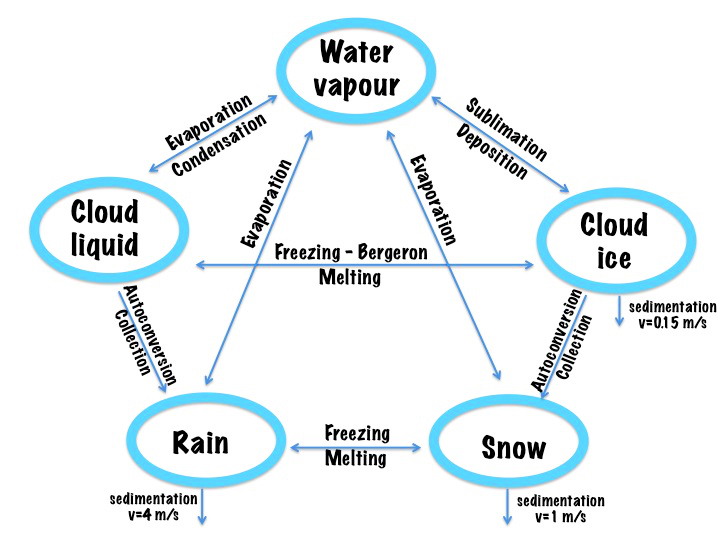
\includegraphics[width=0.6\textwidth]{scheme_var2.jpg}
\end{center}
\caption{\small Schematics of the new scheme, showing the 5 prognostic variables and  how they are related to each other through microphysical processes}
\label{fig:newscheme}
\end{figure}
\noindent microphysical properties (i.e. condensation, evaporation, auto-conversion, melting...), and the sedimentation term, that is a function of the fall speed $V_x$ that has a fixed value for each cloud variable. 
To solve the equations the upstream approach is used.  The sources and sinks contributors are divided in two groups according to the duration of the process they describe: processes that are considered to be fast relative to the timestep of the model are treated implicitly while slow processes are treated explicitly. The processes taken into account (shown in Fig.~\ref{fig:newscheme})) are the microphysical pathways between the 5 considered variables: condensation, autoconversion, evaporation, collection for the warm clouds, and autoconversion, freezing, melting, deposition, evaporation for the cold clouds.\\
For each microphysical pathway the change of phase is associated with a release or an absorption of latent heat, that has a significant impact on the temperature budget.
The impact is calculated using the conservation of liquid water temperature $T_L$ defined as:
\begin{equation}
T_L=T-\frac{L_v}{C_p}(q_l+q_r)-\frac{L_s}{C_p}(q_i+q_s).
\end{equation}
Being that $\frac{dT_L}{dt}=0$, the rate of change of the temperature is  given by the following equation:
\begin{equation}
\frac{\partial T}{\partial t}=\sum_{x=1}^m\frac{L(x)}{C_p}\Big(\frac{dq_x}{dt}-D_{q_x}-\frac{1}{\rho}\frac{\partial}{\partial z}(\rho V_x q_x)\Big)
\end{equation}
where $L(x)$ is the latent heat (of fusion or evaporation depending on the processes considered), $D_{q_x}$ is the convective detrainment and the third term in the brackets is the sedimentation term.\\
At the end of each timestep a routine checks the conservation of the total water and of the moist static energy $h=C_P T+gz+ Lq_x$.

\subsection{Ocean flux Parameterization}

\ac{BATS} uses standard Monin-Obukhov similarity relations to compute the
fluxes with no
special treatment of convective and very stable conditions.  In addition, the
roughness length is set to a constant, i.e. it is not a function of wind and
stability.  

The Zeng scheme describes all stability conditions and
includes a gustiness velocity to account for the additional flux induced by
boundary layer scale variability. Sensible heat (${\rm SH}$), latent heat (${\rm
LH}$), and momentum ($\tau$) fluxes between the sea surface and lower atmosphere
are calculated using the following bulk aerodynamic algorithms,
    
\begin{eqnarray}
\tau = \rho_a {u_{\ast}}^2 ({u_{x}}^2 + {u_{y}}^2)^{1/2} / u \\ \nonumber \\
{\rm SH} = -\rho_a C_{pa} u_{\ast} \theta_{\ast} \hspace{.6cm} \\ \nonumber \\
{\rm LH} =  -\rho_a L_{e} u_{\ast} q_{\ast}  \hspace{.65cm}
\end{eqnarray}

where $u_x$ and $u_y$ are mean wind components, $u_{\ast}$ is the
frictional wind velocity, $\theta_{\ast}$ is the temperature scaling parameter,
$q_{\ast}$ is the specific humidity scaling parameter,  $\rho_a$ is air density,
$C_{pa}$ is specific heat of air, and $L_{e}$ is the latent heat of
vaporization.  For further details on the calculation of these parameters refer
to \cite{Zeng_98}.
 
\subsection{Prognostic Sea Surface Skin Temperature Scheme}

By default in \ac{RegCM}, sea surface temperatures (SST) are prescribed every
six hours from temporally interpolated weekly or monthly SST products.
These products, which are produced from satellite retrievals and in situ
measurements, are representative of the mean temperature in the top
few meters of the ocean. However, the actual SST can differ significantly
from this mean temperature due to the cool-skin and warm-layer effects
described by \cite{Fairall_96}. To improve the calculation of diurnal fluxes
over the ocean, the prognostic SST scheme described by \cite{Zeng_05} was
implemented in \ac{RegCM4}. The scheme is based on a two-layer
one-dimensional heat transfer model, with the top layer representing the
upper few millimeters of the ocean which is cooled by net longwave radiation
loss and surface fluxes. The bottom layer is three meters thick, it is warmer by
solar radiation and exchanges heat with the top layer. This diurnal SST
scheme appears to provide significant, although not major, effects on the
model climatology mostly over tropical oceans, for example the Indian ocean,
and it is now used as default in \ac{RegCM4}.

\subsection{Pressure Gradient Scheme}

Two options are available for
calculating the pressure gradient force.  The normal way uses the full fields.
The other way is the hydrostatic deduction scheme which makes use of a
perturbation temperature.  In this scheme, extra smoothing on the top is done in
order to reduce errors related to the PGF calculation. 

\subsection{Lake Model}
The lake model developed by \cite{Hostetler_93} can
be interactively coupled to the atmospheric model.  In the lake model, fluxes of
heat, moisture, and momentum are calculated based on meteorological inputs and
the lake surface temperature and albedo.  Heat is transferred vertically between
lake model layers by eddy and convective mixing.  Ice and snow may cover part or
all of the lake surface.

In the lake model, the prognostic equation for temperature is

\begin{eqnarray}
{\partial{T}\over \partial{t}} = (k_e + k_m) {\partial^2{T}\over \partial{z}^2 }
\end{eqnarray}

where $T$ is the temperature of the lake layer, and $k_e$ and $k_m$
are the eddy and molecular diffusivities, respectively.   The parameterization
of \cite{Henderson-Sellers_86} is used to calculate $k_e$ and $k_m$ is set to a
constant value of $39 \times 10^{-7}~m^2~s^{-1}$ except under ice and at the
deepest points in the lake.

Sensible and latent heat fluxes from the lake are calculated using  the BATS
parameterizations \cite{Dickinson_93}.  The bulk aerodynamic formulations for
latent heat flux ($F_q$) and sensible heat flux ($F_s$) are as follows,

\begin{eqnarray}
F_q = \rho_a C_D V_a L_v (q_s - q_a) \\ F_s = \rho_a C_p C_D V_a (T_s - T_a)
\end{eqnarray}

where the subscripts $s$ and $a$ refer to surface and air,
respectively; $\rho_a$ is the density of air, $V_a$ is the wind speed, $C_p$
is specific heat at constant pressure, $L_v$ is evaporation latent
heat, $q$ is specific humidity, and $T$ is temperature.  The momentum drag
coefficient, $C_D$, depends on roughness length and the surface bulk Richardson
number.

Under ice-free conditions, the lake surface albedo is calculated as a function
of solar zenith angle \cite{Henderson-Sellers_86}.  Longwave radiation emitted
from the lake is calculated according to the Stefan-Boltzmann law.  The lake
model uses the partial ice cover scheme of \cite{Patterson_88} to represent the
different heat and moisture exchanges between open water and ice surfaces and
the atmosphere, and to calculate the surface energy of lake ice and overlying
snow.  For further details refer to \cite{Hostetler_93} and \cite{Small_99b}. 

\subsection{Aerosols and Dust (Chemistry Model)}

The representation of dust
emission processes is a key element in a dust model and depends on the wind
conditions, the soil characteristics and the particle size. Following
\cite{Marticorena_05} and \cite{Alfaro_01}, here the dust
emission calculation is based on parameterizations of soil aggregate saltation
and sandblasting processes. The main steps in this calculation are: The
specification of soil aggregate size distribution for each model grid cell, the
calculation of a threshold friction velocity leading to erosion and saltation
processes, the calculation of the horizontal saltating soil aggregate mass flux,
and finally the calculation of the vertical transportable dust particle mass
flux generated by the saltating aggregates. In relation to the BATS interface,
these parameterizations become effective in the model for cells dominated by
desert and semi desert land cover. 

\newpage
\section{Pre-Processing}
Before performing a regional climate simulation there are two pre-processing steps that need to be completed.  The first step involves defining the domain and grid interval, and interpolating the landuse and elevation data to the model grid.  This task is performed in the {\bf RegCM/PreProc/Terrain} sub-directory. The second step is to generate the files used for the initial and boundary conditions during the simulation. This step is performed in the {\bf RegCM/PreProc/ICBC} sub-directory.  The input data necessary to run the model can be downloaded from the PWC 
website at the following URL: \\

{\bf http://www.ictp.trieste.it/$\sim$pubregcm/RegCM3} \\

Input data used by the {\bf Terrain} and {\bf ICBC}  programs are 
stored in the {\bf RegCM/PreProc/DATA} sub-directory.  A script called
{\it datalinker.x} is provided in this directory in case the data 
exists elsewhere.  It can be modified and run to create soft links 
between the {\bf RegCM/PreProc/DATA} sub-directory and another directory.

The present version of RegCM3 supports multi-platforms running under a UNIX (or LINUX) operating
system, such as IBM, SGI, SUN, DEC, and PC-LINUX (with PGI FORTRAN compiler (not free) or
Intel IFC FORTRAN compiler (free)). You must make your choices of Makefile under 
PreProc/Terrain, PreProc/ICBC, and Main/ directories by copying the appropriate
Makefile. 

\subsection{Terrain}

The domain for your simulation is defined in {\bf Terrain}. There are several important considerations for choosing the domain
resolution, projection, and resolution. Resolution depends on the
science question you are asking and the available computational
resources. RegCM is a hydrostatic model; therefore, the horizontal grid
spacing should probably not be set lower than 10 km. In general, the
Lambert Conformal Conic projection is used for middle and high latitude
regions, while the standard Mercator and rotated Mercator projections
are used in tropical and subtropical regions.  When choosing the model's central point (clat, clon) and map projection, it is important to
make the whole domain map factor as close to 1 as possible, which will be helpful for model's computational stability. The map factor can be checked using the DOMAIN\_INFO.CTL and DOMAIN\_INFO files in GrADS.

As for the choice of the
domain itself, it depends on the area of interest and the application.
The regional model solution is a combination of the lateral boundary
forcing and the internal model physics. With a smaller domain, the
lateral boundary conditions exert more control. This may be desirable
for seasonal prediction (although large domains can also be used for this purpose) or other applications. For sensitivity studies
such as changing land cover or soil moisture, a larger domain may be
preferable since it allows for more internal model freedom to respond to
the applied changes \citep{Seth_98}. The issue of computational cost and managing the
output data is also important. For every doubling (2x) of the number of horizontal grid points, the computational time (assuming the same horizontal grid spacing) increases by a factor of 4. Output data increase slightly less than a factor of 4, since not all RegCM3 output is three-dimensional. Still, it is important to note that data storage can be as expensive in the long term as running the simulation. 

There are some papers (\citet{Seth_98,Vannitsem_05,Rauscher_06a})
that discuss domain choice in more depth.


\begin{table}
\begin{center}
\caption{Land Cover/Vegetation classes} \label{VegTypes}
\begin{tabular}{rl}
\hline\hline
1.&Crop/mixed farming\\
2.&Short grass\\
3.&Evergreen needleleaf tree\\
4.&Deciduous needleleaf tree\\
5.&Deciduous broadleaf tree\\
6.&Evergreen broadleaf tree\\
7.&Tall grass\\
8.&Desert\\
9.&Tundra\\
10.&Irrigated Crop\\
11.&Semi-desert\\
12.&Ice cap/glacier\\
13.&Bog or marsh\\
14.&Inland water\\
15.&Ocean\\
16.&Evergreen shrub\\
17.&Deciduous shrub\\
18.&Mixed Woodland\\
19.&Forest/Field mosaic \\
20.&Water and Land mixture \\
\hline\hline
\end{tabular}
\end{center}
\end{table}

\begin{center}
\begin{landscape}
\begin{table}
%\scriptsize{
\caption{BATS vegetation/land-cover}  \label{landuse}
\hspace{-0.8cm}
%\vspace{-2.0cm}
\begin{tabular}{lcccccccccccccccccccc} \hline \hline
\multicolumn{1}{c}{Parameter}&\multicolumn{20}{c}{Land Cover/Vegetation Type}\\
&1&2&3&4&5&6&7&8&9&10&11&12&13&14&15&16&17&18&19&20 \\ \hline
Max fractional \\
vegetation cover&0.85&0.80&0.80&0.80&0.80&0.90&0.80&0.00&0.60&0.80&0.35&0.00&0.80&0.00&0.00&0.80&0.80&0.80&0.80&0.80 \\
Difference between max\\
fractional vegetation \\
cover and cover at 269 K&0.6&0.1&0.1&0.3&0.5&0.3&0.0&0.2&0.6&0.1&0.0&0.4&0.0&0.0&0.2&0.3&0.2&0.4&0.4 \\
Roughness length (m)       &0.08&0.05&1.00&1.00&0.80&2.00&0.10&0.05&0.04&0.06&0.10&0.01&0.03&0.0004&0.0004&0.10&0.10&0.80&0.3&0.3 \\
Displacement height (m)    &0.0&0.0&9.0&9.0&0.0&18.0&0.0&0.0&0.0&0.0&0.0&0.0&0.0&0.0&0.0&0.0&0.0&0.0&0.0&0.0 \\
Min stomatal \\
resistence (s/m)  &45 &60 &80 &80 &120 &60 &60 &200 &80 &45 &150 &200 &45 &200 &200 &80 &120 &100&120&120  \\
Max Leaf Area Index            &6   &2   &6   &6   &6   &6   &6   &0   &6   &6   &6   &0   &6   &0   &0   &6   &6   &6 &6 &6    \\
Min Leaf Area Index            &0.5 &0.5 &5   &1   &1   &5   &0.5 &0   &0.5 &0.5 &0.5 &0   &0.5 &0   &0   &5   &1   &3  &0.5 &0.5   \\
Stem (dead matter \\
area index)&0.5&4.0&2.0&2.0&2.0&2.0&2.0&0.5&0.5&2.0&2.0&2.0&2.0&2.0&2.0&2.0&2.0&2.0&2.0&2.0 \\
Inverse square root of \\
leaf dimension (m$^{-1/2}$)&10&5&5&5&5&5&5&5&5&5&5&5&5&5&5&5&5&5&5&5\\
Light sensitivity \\
factor (m$^2$ W$^{-1}$)&0.02&0.02&0.06&0.06&0.06&0.06&0.02&0.02&0.02&0.02&0.02&0.02&0.02&0.02&0.02&0.02&0.02&0.06&0.02&0.02 \\ 
Upper soil layer \\
depth (mm)     &100 &100 &100 &100 &100 &100 &100 &100 &100 &100 &100 &100 &100 &100 &100 &100 &100 &100 &100 &100  \\
Root zone soil\\
layer depth (mm) &1000 &1000 &1500 &1500 &2000 &1500 &1000 &1000 &1000 &1000 &1000 &1000 &1000 &1000 &1000 &1000 &1000 &2000 &2000 &2000  \\
Depth of total\\
soil (mm) &3000 &3000 &3000 &3000 &3000 &3000 &3000 &3000 &3000 &3000 &3000 &3000 &3000 &3000 &3000 &3000 &3000 &3000 &3000 &3000  \\
Soil texture type    &6   &6   &6   &6   &7   &8   &6   &3   &6   &6   &5   &12   &6   &6   &6   &6   &5   &6 &6 &0    \\
Soil color type    &5   &3   &4   &4   &4   &4   &4   &1   &3   &3   &2   &1   &5   &5   &5   &4   &3   &4 &4 &0    \\
Vegetation albedo for \\
wavelengths $<$ 0.7 $\mu$ m &0.10&0.10&0.05&0.05&0.08&0.04&0.08&0.20&0.10&0.08&0.17&0.80&0.06&0.07&0.07&0.05&0.08&0.06 &0.06 &0.06 \\
Vegetation albedo for \\
wavelengths $>$ 0.7 $\mu$ m &0.30&0.30&0.23&0.23&0.28&0.20&0.30&0.40&0.30&0.28&0.34&0.60&0.18&0.20&0.20&0.23&0.28&0.24&0.18&0.18 \\  \hline \hline
\end{tabular}
\end{table}
\end{landscape}
\end{center}

The Terrain program horizontally interpolates the landuse and elevation data from a latitude-longitude grid to the cartesian grid of the chosen domain. RegCM currently uses the Global Land Cover Characterization (GLCC) datasets for the vegetation/landuse data.  The GLCC dataset is derived from 1~km Advanced Very High Resolution Radiometer (AVHRR) data spanning April 1992 through March 1993, and is based on the vegetation/land cover types defined by BATS (Biosphere Atmosphere Transfer Scheme).  The 20 vegetation/land cover types and associated parameters are presented in Table~\ref{landuse}. Each grid cell of the model is assigned one of the eighteen 
categories. More information regarding GLCC datasets can be found at {\bf http://edcdaac.usgs.gov/glcc/glcc.html}.

The elevation data used is from the United States Geological Survey (USGS).Both the landuse and elevation data files are available at 60, 30, 10, 5, 3, and 2 minute resolutions and can be downloaded from the ICTP~PWC website at {\bf http://www.ictp.trieste.it/$\sim$pubregcm/RegCM3/globedat.htm}.

\begin{table}[h]
\begin{center}
\caption{List of variables defined in {\it domain.param} file.}  \label{domain.param_file}
\vspace{0.25cm}
\begin{tabular}{|l|l|} \hline \hline
{\small {\bf Parameter}}   &   {\small {\bf Description}} \\ \hline \hline
{\footnotesize {\bf iproj}}    & {\footnotesize map projection} \\ 
 &  \vspace{-0.15 cm} \hspace{0.5 cm} {\footnotesize 'LAMCON' = Lambert Conformal } \\
 &  \vspace{-0.15 cm} \hspace{0.5 cm} {\footnotesize 'POLSTR' = Polar Stereographic } \\ 
 &  \vspace{-0.15 cm} \hspace{0.5 cm} {\footnotesize 'NORMER' = Normal Mercator} \\
 &  \hspace{0.5 cm} {\footnotesize 'ROTMER' = Rotated Mercator} \\ \hline
{\footnotesize {\bf iy}}   &   {\footnotesize number of grid points in y direction (i)} \\ \hline
{\footnotesize {\bf jx}}   &   {\footnotesize number of grid points in x direction (j)} \\ \hline
{\footnotesize {\bf kz}}   &   {\footnotesize number of vertical levels (k)} \\ \hline
{\footnotesize {\bf nsg}}  &   {\footnotesize number of subgrids in one direction} \\ \hline
{\footnotesize {\bf ds}}   &   {\footnotesize grid point separation in km} \\ \hline
{\footnotesize {\bf ptop}} &   {\footnotesize pressure of model top in cb} \\ \hline
{\footnotesize {\bf clat}} &   {\footnotesize central latitude of model domain in degrees} \\  \hline
{\footnotesize {\bf clon}} &   {\footnotesize central longitude of model domain in degrees} \\  \hline
{\footnotesize {\bf plat}} &   {\footnotesize pole latitude (only for rotated mercator projection)} \\  \hline
{\footnotesize {\bf plon}} &   {\footnotesize pole longitude (only for rotated mercator projection)} \\  \hline
{\footnotesize {\bf truelatL}} &   {\footnotesize Lambert true latitude (low  latitude side)} \\  \hline
{\footnotesize {\bf truelon}} &   {\footnotesize Lambert true latitude (high latitude side)} \\  \hline
{\footnotesize {\bf ntypec}} & {\footnotesize resolution of the global terrain and land-use data} \\
 &  \vspace{-0.15 cm} \hspace{0.5 cm} {\footnotesize 60 = 1 degree \hspace{1.25cm} 5 = 5 minute} \\ 
 &  \vspace{-0.15 cm} \hspace{0.5 cm} {\footnotesize 30 = 30 minute \hspace{1.1cm} 3 = 3 minute} \\ 
 &  \hspace{0.5 cm} {\footnotesize 10 = 10 minute \hspace{1cm} 2 = 2 minute } \\ \hline
{\footnotesize {\bf ntypec\_s}} & {\footnotesize same as ntypec, except for subgrid} \\ \hline

{\footnotesize {\bf h2opct}}  & {\footnotesize if water percentage $<$ h2opct, then land else water} \\ \hline
{\footnotesize {\bf ifanal}}  & {\footnotesize  true=perform cressman-type objective analysis} \\  
 & {\footnotesize  false=perform 16-point overlapping parabolic interpolation} \\ \hline
{\footnotesize {\bf smthbdy}}  & {\footnotesize true=extra smoothing in boundaries} \\ \hline
{\footnotesize {\bf lakadj}}   & {\footnotesize true=adjust lake levels according to obs} \\ \hline
{\footnotesize {\bf igrads}}   & {\footnotesize true=output GrADS control file} \\ \hline
{\footnotesize {\bf ibigend}}  & {\footnotesize 1 = big-endian (always 1)} \\ \hline
{\footnotesize {\bf ibyte}}  & {\footnotesize for direct access open statements (1 or 4)} \\  
 & {\footnotesize  1 for IFC8, SGI, DEC;  4 for PGI, IFC7, SUN, IBM} \\ \hline

{\footnotesize {\bf FUDGE\_LND}}   & {\footnotesize land use fudge, true or false} \\ \hline
{\footnotesize {\bf FUDGE\_TEX}}   & {\footnotesize texture fudge, true or false} \\ \hline
{\footnotesize {\bf FUDGE\_LND\_s}} & {\footnotesize land use fudge for subgrid, true or false} \\ \hline
{\footnotesize {\bf FUDGE\_TEX}}   & {\footnotesize texture fudge for subgrid, true or false} \\ \hline
{\footnotesize {\bf filout}}   & {\footnotesize terrain output filename including path} \\ \hline
{\footnotesize {\bf filctl}}   & {\footnotesize GrADS control filename for output including path} \\ \hline
{\footnotesize {\bf IDATE1}}   & {\footnotesize beginning date of simulation (YYYYMMDDHH)} \\ \hline
{\footnotesize {\bf IDATE2}}   & {\footnotesize ending date of simulation (YYYYMMDDHH)} \\ \hline
{\footnotesize {\bf DATTYP}}   & {\footnotesize global analysis dataset} \\ 
 &  \vspace{-0.15 cm} \hspace{0.5 cm} {\footnotesize 'ECMWF'} \hspace{0.5 cm} {\footnotesize 'ERA40'}  \hspace{0.5 cm} {\footnotesize 'ERAHI'} \\
 &  \vspace{-0.15 cm}\hspace{0.5 cm} {\footnotesize 'NNRP1'} \hspace{0.5 cm} {\footnotesize 'NNRP2'} \hspace{0.5 cm} {\footnotesize 'NRP2W'}\\
 &  \vspace{-0.15 cm} \hspace{0.5 cm} {\footnotesize 'FVGCM'} \hspace{0.5 cm} {\footnotesize 'FNEST'} \hspace{0.5 cm} {\footnotesize 'EH50M'}\\
\hline
{\footnotesize {\bf SSTTYP}}  & {\footnotesize SST dataset } \\ 
 &  \vspace{-0.15 cm} \hspace{0.5 cm} {\footnotesize 'GISST'} \hspace{0.5 cm} {\footnotesize 'OISST'} \hspace{0.5 cm} {\footnotesize 'OI\_NC'} \hspace{0.5 cm} {\footnotesize 'OI\_WK'}\\ 
 &  \vspace{-0.15 cm} \hspace{0.5 cm} {\footnotesize for FVGCM:} \hspace{0.5 cm} {\footnotesize 'FV\_RF'}  \hspace{0.5 cm} {\footnotesize 'FV\_A2'}\\
 &  \vspace{-0.15 cm} \hspace{0.5 cm} {\footnotesize for ECHAM GCM:} \hspace{0.5 cm} {\footnotesize 'EH5RF'}  \hspace{0.5 cm} {\footnotesize 'EH5A2'}\\
\hline
{\footnotesize {\bf LSMTYP}} & {\footnotesize LANDUSE legend, 'BATS' or 'USGS'} \\ \hline
{\footnotesize {\bf AERTYP}} & {\footnotesize AEROSOL datasets:}\\
 &  \vspace{-0.15 cm} \hspace{0.5 cm} {\footnotesize 'AER00D0'} \hspace{0.5 cm} {\footnotesize Neither aerosol, nor dust used}\\
 &  \vspace{-0.15 cm} \hspace{0.5 cm} {\footnotesize 'AER01D0'} \hspace{0.5 cm} {\footnotesize Biomass, SO2 + BC + OC, no dust}\\ 
 &  \vspace{-0.15 cm} \hspace{0.5 cm} {\footnotesize 'AER10D0'} \hspace{0.5 cm} {\footnotesize Anthropogenic, SO2 + BC + OC, no dust}\\
 &  \vspace{-0.15 cm} \hspace{0.5 cm} {\footnotesize 'AER11D0'} \hspace{0.5 cm} {\footnotesize Anthropogenic+Biomass, SO2 + BC + OC, no dust}\\
 &  \vspace{-0.15 cm} \hspace{0.5 cm} {\footnotesize 'AER00D1'} \hspace{0.5 cm} {\footnotesize No aerosol, with dust}\\
&  \vspace{-0.15 cm} \hspace{0.5 cm} {\footnotesize 'AER01D1'}  \hspace{0.5 cm} {\footnotesize Biomass, SO2 + BC + OC, with dust}\\
&  \vspace{-0.15 cm} \hspace{0.5 cm} {\footnotesize 'AER10D1'}  \hspace{0.5 cm} {\footnotesize Anthropogenic, SO2 + BC + OC, with dust}\\
&  \vspace{-0.15 cm} \hspace{0.5 cm} {\footnotesize 'AER11D1'}  \hspace{0.5 cm} {\footnotesize Anthropogenic+Biomass, SO2 + BC + OC, with dust.}\\
\hline
{\footnotesize {\bf ntex}}   & {\footnotesize Number of SOIL TEXTURE categories, 17} \\ \hline
{\footnotesize {\bf NPROC}}   & {\footnotesize Number of CPU used for parallel run.} \\ \hline
\hline
\end{tabular}
\end{center}
\end{table}

Parameters such as domain size, input data, and length of simulation are defined in the file {\it domain.param} (Table~\ref{domain.param_file}) under directory {\bf RegCM/PreProc/Terrain/}.  After editing this file, running the {\it terrain.x} script will compile and execute the terrain program.  This will generate the output file {\it DOMAIN.INFO} containing elevation, landuse type, and other variables (Table~\ref{ter_var})  in the {\bf RegCM/Input} sub-directory.  A GrADS descriptor file, {\it DOMAIN.CTL} is also created.

In case you are not satisfied with the landuse pattern over your domain, you 
can modify the landuse values assigned to individual grid points by modifying the
{\bf RegCM/PreProc/Terrain/}{\it LANDUSE} file and changing the FUDGE\_LND parameter (and/or FUDGE\_LND\_s for sub-BATS) in the
{\bf RegCM/PreProc/Terrain/}{\it domain.param} file to be true.  The {\it LANDUSE} file 
contains the land cover/vegetation classes (Table~\ref{VegTypes}) assigned to all 
of the grid points in your domain.  Land cover/vegetation classes 10--20 are 
represented with single characters from A--K, in which A represents class 10, 
B represents class 11, etc.  After you modify the {\it LANDUSE} and change the
FUDGE\_LND and FUDGE\_LND\_s parameters in the {\it domain.param} file, you must re-run the terrain 
program.

\begin{table}[h]
\begin{center}
\caption{List of output variables from Terrain (DOMAIN)}  \label{ter_var}
\vspace{0.25cm}
\begin{tabular}{|l|c|l|} \hline \hline
{\small {\bf Variables}} & {\small {\bf Description}} \\ \hline \hline
{\ {\bf ht}}    & {\ {Surface elevation (m)} }      \\ \hline
{\ {\bf htsd}}    & {\ {Surface elevation standard deviation} }    \\ \hline
{\ {\bf landuse}}    & {\ {Surface landuse type}}       \\ \hline
{\ {\bf xlat}}    & {\ {Latitude of cross points} }      \\ \hline
{\ {\bf xlon}}    & {\ {Longitude of cross points}}   \\ \hline
{\ {\bf dlat}}    & {\ {Latitude of dot points}}       \\ \hline
{\ {\bf dlon}}    & {\ {Longitude of dot points} }      \\ \hline
{\ {\bf xmap}}    & {\ {Map factors of cross points} }     \\ \hline
{\ {\bf dmap}}    & {\ {Map factors of dot points}}       \\ \hline
{\ {\bf coriol}}    & {\ {Coriolis force} }      \\ \hline
{\ {\bf snowam}}    & {\ {Initial snow amount} }     \\ \hline
{\ {\bf mask}}    & {\ {land/sea mask} }     \\ \hline
{\ {\bf texture}}    & {\ {Soil texture} }     \\ \hline
\end{tabular}
\end{center}
\end{table}

\subsection{ICBC}
The ICBC program interpolates sea surface temperature (SST) and global re-analysis data to the model grid.  These files are used for the initial and boundary conditions during the simulation. 

\subsubsection{Sea surface temperature}     

In the {\bf RegCM/PreProc/Terrain/}{\it domain.param} file, there are several 
options for SST data, including the Global Sea Surface Temperature (GISST) 
one-degree monthly gridded data (1871-2002) available from the Hadley Centre 
Met Office at http://badc.nerc.ac.uk/data/gisst/. Please note that permission is needed from the Hadley Center Met Office to use the GISST datasets. Also available is the 
Optimum Interpolation Sea Surface Temperature (OISST) one-degree (1981-2005) available from the National Ocean and Atmosphere Administration at both weekly and monthly time scales at http://www.cdc.noaa.gov/. Additionally, SSTs for climate change reference and scenario runs may also be used.

\subsubsection{Data for Initial and Lateral Boundary Conditions}

In the {\bf RegCM/PreProc/Terrain/}{\it domain.param} file, there are several data sets that can be chosen to use for the initial and boundary conditions.  

$\bullet$  {\bf ECMWF}:  The European Centre for Medium-Range Weather Forecasts
Reanalysis datasets (T42,L15) from 1993--1997. 

$\bullet$  {\bf ERA40}:  ECMWF 40 year reanalysis datasets (2.5 degree grid,L23) from 1957--2002. 

$\bullet$  {\bf ERAHI}: ECMWF 40 year reanalysis datasets, original model level fields:
 T, U, V and log(Ps) are in spectral coefficients; orography and Q are at the reduced Gaussian grids. T159L60 (N80L60) from 1957--2002 

$\bullet$  {\bf NNRP1}:  The National Center for Environmental Prediction  (NCEP) 
Reanalysis datasets (2.5 degree grid, L17) from 1948--present. 

$\bullet$  {\bf NNRP2}:  The National Center for Environmental Prediction  (NCEP) 
Reanalysis datasets (2.5 degree grid, L17) from 1979--2005. 

$\bullet$  {\bf NRP2W}: Small Window (instead of global) of NNRP2 to save disk space. (For example, African window: 40W to 80E, 60S to 70N) 

$\bullet$  {\bf FVGCM}:  For climate change experiments you can use output from the NASA-NCAR finite volume GCM to drive RegCM.  We have run FVGCM (1 x 1.25 degree grid, L18) here at ICTP and have output available from four 30-year simulations. Two present day reference runs from 1961--1990 and two future A2 IPCC emission scenario runs from 2071--2100.  

$\bullet$  {\bf EH50M}: From EC-Hamburg coupled GCM IPCC AR4 experiments (AGCM: Echam5, T63L31; OGCM: MPI-OM GR1.5 256x220L40; Coupler: OASIS), 20C (1950-2000) and A1B (2001-2100) IPCC Emission Senario, T63, reformated pressure layer data.

$\bullet$  {\bf FNEST}:  A one-way nesting option is available for high resolution RegCM simulations in which output from a coarse resolution RegCM simulation are used drive the model at a higher resolution over a subregion. 

\subsubsection{Lateral Boundary Treatment}

\noindent The numerical treatment of the lateral boundaries is a complex but very 
important aspect of the regional climate model. There are five types of boundary conditions that can be used in the model. The type of boundary conditions used in the simulation is selected in the {\bf RegCM/PreProc/Terrain/}{\it domain.param} file. The options are:

${\bullet}$  {\bf Fixed}: This will not allow time variation at lateral boundaries. Not recommended for real-data applications.

${\bullet}$   {\bf Time-dependent}:  Outer two rows and columns have specified values of all predicted fields. Recommended for nests where time-dependent values are supplied by the parent domain. Not recommended for coarse mesh where only one outer row and column would be specified. 

${\bullet}$    {\bf Linear relaxation}: Outer row and column is specified by time-dependent value, next four points are relaxed towards the boundary values with a relaxation constant that decreases linearly away from the boundary.

${\bullet}$    {\bf Sponge}:  \cite{Perkey_76}

${\bullet}$    {\bf Exponential relaxation}:  \cite{Davies_77}  (default) 


\begin{table}[!]
\begin{center}
\caption{List of variables in {\it ICBCYYYYMMDDHH} files}  \label{icbc_vars}
\vspace{0.25cm}
\begin{tabular}{|l|c|l|} \hline \hline
{\small {\bf Variables}} & {\small {\bf Description}} \\ \hline \hline
{\ {\bf date}}    & {\ {Date of simulation (header information) } }      \\ \hline
{\ {\bf u}}    & {\ {Westerly wind (${\rm m~s^{-1}}$) } }      \\ \hline
{\ {\bf v}}    & {\ {Southerly wind (${\rm m~s^{-1}}$)} }     \\ \hline
{\ {\bf t}}    & {\ {Air temperature (K)}}       \\ \hline
{\ {\bf q}}    & {\ {Specific moisture (${\rm kg~kg^{-1}}$)} }      \\ \hline
{\ {\bf px}}    & {\ {Surface pressure (hPa)} }     \\ \hline
{\ {\bf ts}}    & {\ {Surface air temperature (K)}}       \\ \hline
\end{tabular}
\end{center}
\end{table}

\subsubsection{Running ICBC}
\noindent It is not necessary to modify any files in the  {\bf RegCM/PreProc/ICBC} 
sub-directory. The {\it SST\_1DEG.f} and {\it ICBC.f} programs interpolate 
the SST and global analysis data to the model grid.  Running the 
{\it icbc.x} script will compile and execute these programs.  The following 
files will be generated; \\ 

\indent {\bf RegCM/Input/}{ICBC.YYYYMMDDHH} (see Table~\ref{icbc_vars} for list of variables) \\
\indent {\bf RegCM/Input/}{ICBC.YYYYMMDDHH.CTL}  \\

\noindent However, if you want to start a new simulation but do not need to modify your
domain then you can simply edit the date parameters in the {\bf RegCM/PreProc/ICBC}
{\it icbc.param} file before running the {\it icbc.x} script.



\section{RegCM}
\begin{table}[h]
\begin{center}
\caption{List of restart, timestep, and output parameters defined in {\it regcm.in} file.}  \label{regcm.in_file}
\vspace{0.25cm}
\begin{tabular}{|l|l|} \hline \hline
{\small {\bf Restart parameters}} &   {\small {\bf Description}} \\ \hline \hline
{\footnotesize {\bf ifrest}} & {\footnotesize true or false for restart simulation} \\ \hline
\hspace{.3cm} {\footnotesize {\bf idate0}} & {\footnotesize start date of first simulation} \\ \hline
\hspace{.3cm} {\footnotesize {\bf idate1}} & {\footnotesize restart date} \\ \hline
\hspace{.3cm} {\footnotesize {\bf idate2}} & {\footnotesize end date of restart simulation} \\ \hline
{\footnotesize {\bf nslice}} & {\footnotesize number of days for next model run} \\ \hline \hline
{\small {\bf Timestep parameters}} &   {\small {\bf Description}} \\ \hline \hline
{\footnotesize {\bf radfrq}} & {\footnotesize time step for radiation model} \\ \hline
\hspace{.3cm} {\footnotesize {\bf abemh}}  & {\footnotesize time step for LW absorption/emissivity} \\ \hline
{\footnotesize {\bf abatm}}  & {\footnotesize time step for lsm} \\ \hline
{\footnotesize {\bf dt}}     & {\footnotesize time step for atmosphere model} \\ \hline
{\footnotesize {\bf ibdyfrq}} & {\footnotesize lateral boundary conditions frequency} \\ \hline \hline
{\small {\bf Output parameters}} &   {\small {\bf Description}} \\ \hline \hline
{\footnotesize {\bf ifsave}} & {\footnotesize save output for restart} \\ \hline
\hspace{.3cm} {\footnotesize {\bf savfrq}} & {\footnotesize time interval to save output for restart (hr)} \\ \hline
{\footnotesize {\bf iftape}} & {\footnotesize save atmospheric output} \\ \hline
\hspace{.3cm} {\footnotesize {\bf tapfrq}} & {\footnotesize time interval to save atmospheric output (hr)} \\ \hline
{\footnotesize {\bf ifrad}}  & {\footnotesize save radiation output } \\ \hline
\hspace{.3cm} {\footnotesize {\bf radisp}} & {\footnotesize time interval to save radiation output (hrs) } \\  \hline
{\footnotesize {\bf ifbat}}  & {\footnotesize save surface model output } \\  \hline
{\footnotesize {\bf ifsub}}  & {\footnotesize save sub-bats model output } \\  \hline
\hspace{.3cm} {\footnotesize {\bf batfrq}} & {\footnotesize time interval to save surface model output (hrs) }  \\ \hline
{\footnotesize {\bf ifprt}}  & {\footnotesize printer output} \\ \hline
\hspace{.3cm} {\footnotesize {\bf prtfrq}} & {\footnotesize time interval for printer output (hrs)} \\ \hline
\hspace{.3cm} {\footnotesize {\bf kxout}}  & {\footnotesize k level of horizontal slice for printer output} \\ \hline
\hspace{.3cm} {\footnotesize {\bf jxsex}}  & {\footnotesize j index of the north-south vertical slice for printer output} \\ \hline
{\footnotesize {\bf iotyp}}  & {\footnotesize Output format; 1=direct access, 2=sequential} \\ \hline
\hspace{.3cm} {\footnotesize {\bf ibintyp}}  & {\footnotesize 1=big\_endian, 2=little\_endian} \\ \hline
{\footnotesize {\bf ifchem}}  & {\footnotesize save tracer model output } \\ \hline
\hspace{.3cm} {\footnotesize {\bf chemfrq}} & {\footnotesize time interval to save tracer model output (hrs) } \\  \hline
\end{tabular}
\end{center}
\end{table}

\begin{table}[h]
\begin{center}
\caption{List of physic options in {\it regcm.in} file.}  \label{regcm_file2}
\vspace{0.25cm}
\begin{tabular}{|l|l|} \hline \hline
{\small {\bf Physics parameter}} & {\small {\bf Description}} \\ \hline \hline
{\footnotesize {\bf iboudy}}   & {\footnotesize lateral boundary conditions; 0=fixed, 1=relaxation (linear),} \\ 
  &  {\footnotesize 2=time dependent, 3=time and inflow/outflow dependent} \\
  &  {\footnotesize 4=sponge, 5=relaxation (exponential)} \\ \hline
{\footnotesize {\bf ibltyp}}   &  {\footnotesize planetary boundary layer scheme; 1=Holtslag} \\ \hline
{\footnotesize {\bf icup}}     & {\footnotesize cumulus scheme; 1=Anthes-Kuo, 2=Grell, 4=MIT-Emanuel}  \\ \hline
\hspace{.3cm} {\footnotesize {\bf igcc}}     & {\footnotesize Grell Scheme Convective Closure Scheme;} \\ 
  & {\footnotesize 1=Arakawa \& Schubert, 2=Fritsch \& Chappell} \\ \hline
{\footnotesize {\bf ipptls}}   & {\footnotesize Large-scale precipitation scheme; 1=SUBEX} \\ \hline
{\footnotesize {\bf iocnflx}}  & {\footnotesize ocean flux parameterization scheme;  1= BATS, 2=Zeng}\\ \hline
{\footnotesize {\bf ipgf}}     & {\footnotesize pressure gradient scheme; 0=normal way, 1= hydrostatic deduction} \\ \hline
{\footnotesize {\bf lakemod}}  & {\footnotesize Lake model;  0=no, 1=yes} \\ \hline
{\footnotesize {\bf ichem}}  & {\footnotesize Tracer/Chemistry  model;  0=no, 1=yes} \\ \hline
{\small {\bf Chemistry parameters}} & {\small {\bf Description}} \\ \hline \hline
{\footnotesize {\bf idirect}}   & {\footnotesize direct radiative effect of aerosols } \\ \hline
{\footnotesize {\bf chtrname}}   & {\footnotesize Chemistry tracer name} \\ \hline
{\footnotesize {\bf chtrsol}}   & {\footnotesize } \\ \hline
{\footnotesize {\bf chtrdpv}}   & {\footnotesize } \\ \hline
{\footnotesize {\bf dustbsiz}}   & {\footnotesize } \\ \hline
\end{tabular}
\end{center}
\end{table}


\begin{table}[!]
\begin{center}
\caption{List of output variables from atmosphere}  \label{atmos_var}
\vspace{0.25cm}
\begin{tabular}{|l|c|l|} \hline \hline
{\small {\bf Variables}} & {\small {\bf Description}} \\ \hline \hline
{\ {\bf u}}    & {\ {Eastward wind (${\rm m~s^{-1}}$) } }      \\ \hline
{\ {\bf v}}    & {\ {Northward wind (${\rm m~s^{-1}}$)} }     \\ \hline
{\ {\bf w}}    & {\ {Omega (hPa) p-velocity}}       \\ \hline
{\ {\bf t}}    & {\ {Temperature (K)}}       \\ \hline
{\ {\bf qv}}    & {\ {Water vaporMixing ratio (${\rm g~kg^{-1}}$)} }      \\ \hline
{\ {\bf qc}}    & {\ {Cloud water mixing ratio (${\rm g~kg^{-1}}$)} }     \\ \hline
{\ {\bf psa}}    & {\ {Surface pressure (Pa)}}       \\ \hline
{\ {\bf tpr}}    & {\ {Total precipitation (mm)} }      \\ \hline
{\ {\bf tgb}}    & {\ {Lower soil layer temp (K)} }     \\ \hline
{\ {\bf smt}}    & {\ {Total soil water (mm)}}       \\ \hline
{\ {\bf rno}}    & {\ {Base flow (${\rm mm~day^{-1}}$)}}       \\ \hline
\end{tabular}
\end{center}
\end{table}

\begin{table}[!]
\begin{center}
\caption{List of output variables from surface model}  \label{lsm_var}
\vspace{0.25cm}
\begin{tabular}{|l|c|l|} \hline \hline
{\small {\bf Variables}} & {\small {\bf Description}} \\ \hline \hline
{\ {\bf u10m}}    & {\ {Anemometer eastward wind (${\rm m~s^{-1}}$)} }      \\ \hline
{\ {\bf v10m}}    & {\ {Anemometer northward wind (${\rm m~s^{-1}}$)} }     \\ \hline
{\ {\bf uvdrag}}    & {\ {Surface drag stress}}       \\ \hline
{\ {\bf tgb}}    & {\ {Ground temperature (K)} }      \\ \hline
{\ {\bf tlef}}    & {\ {Foliage temperature (K)} }     \\ \hline
{\ {\bf t2m}}    & {\ {Anemometer temperature (K)}}       \\ \hline
{\ {\bf q2m}}    & {\ {Anemometer specific humidity ${\rm kg~kg^{-1}}$ } }      \\ \hline
{\ {\bf ssw}}    & {\ {Top layer soil moisture (mm)} }     \\ \hline
{\ {\bf rsw}}    & {\ {Root layer soil moisture (mm)}}       \\ \hline
{\ {\bf tpr}}    & {\ {Total precipitation (${\rm mm~day^{-1}}$)} }      \\ \hline
{\ {\bf evp}}    & {\ {Evapotranspiration (${\rm mm~day^{-1}}$)} }     \\ \hline
{\ {\bf runoff}}    & {\ {Surface runoff (${\rm mm~day^{-1}}$)}}       \\ \hline
{\ {\bf scv}}    & {\ {Snow water equivalent (mm)} }      \\ \hline
{\ {\bf sena}}    & {\ {Sensible heat (${\rm W~m^{-2}}$)} }     \\ \hline
{\ {\bf flw}}    & {\ {Net longwave (${\rm W~m^{-2}}$)}}       \\ \hline
{\ {\bf fsw}}    & {\ {Net solar absorbed (${\rm W~m^{-2}}$)} }      \\ \hline
{\ {\bf flwd}}   & {\ {Downward longwave (${\rm W~m^{-2}}$)} }     \\ \hline
{\ {\bf sina}}    & {\ {Solar incident (${\rm W~m^{-2}}$)}}       \\ \hline
{\ {\bf prcv}}    & {\ {Convective precipitation (${\rm mm~day^{-1}}$)} }      \\ \hline
{\ {\bf psb}}    & {\ {Surface pressure (Pa)} }     \\ \hline
{\ {\bf zpbl}}    & {\ {PBL height (m)}}       \\ \hline
{\ {\bf tgmax}}    & {\ {maximum ground temperature (K)}}       \\ \hline
{\ {\bf tgmin}}    & {\ {minimum ground temperature (K)}}      \\ \hline
{\ {\bf t2max}}    & {\ {maximum 2m temperature (K)}}     \\ \hline
{\ {\bf t2min}}    & {\ {minimum 2m temperature (K)}}       \\ \hline
{\ {\bf w10max}}    & {\ {maximum 10m wind speed ($ m~s^{-1}$)}}     \\ \hline
{\ {\bf psmin}}    & {\ {minimum surface pressure ($hPa$)}}       \\ \hline

\end{tabular}
\end{center}
\end{table}

\begin{table}[!]
\begin{center}
\caption{List of output variables from radiation model}  \label{rad_var}
\vspace{0.25cm}
\begin{tabular}{|l|c|l|} \hline \hline
{\small {\bf Variables}} & {\small {\bf Description}} \\ \hline \hline
{\ {\bf fc}}    & {\ {Cloud fraction (fraction)} }      \\ \hline
{\ {\bf clwp}}    & {\ {Cld liquid ${\rm H_2O}$ path (${\rm g~m^{-2}}$)} }    \\ \hline
{\ {\bf qrs}}    & {\ {Solar heating rate (${\rm K~s^{-1}}$)}}       \\ \hline
{\ {\bf qrl}}    & {\ {LW cooling rate (${\rm K~s^{-1}}$)} }      \\ \hline
{\ {\bf fsw}}    & {\ {Surface abs solar (${\rm W~m^{-2}}$)} }     \\ \hline
{\ {\bf flw}}    & {\ {LW cooling of surface (${\rm W~m^{-2}}$)}}       \\ \hline
{\ {\bf clrst}}    & {\ {Clear sky col abs sol (${\rm W~m^{-2}}$)} }      \\ \hline
{\ {\bf clrss}}    & {\ {Clear sky surf abs sol (${\rm W~m^{-2}}$)} }     \\ \hline
{\ {\bf clrlt}}    & {\ {Clear sky net up flux (${\rm W~m^{-2}}$)}}       \\ \hline
{\ {\bf clrls}}    & {\ {Clear sky LW surf cool (${\rm W~m^{-2}}$)} }      \\ \hline
{\ {\bf solin}}    & {\ {Instant incid solar (${\rm W~m^{-2}}$)} }     \\ \hline
{\ {\bf sabtp}}    & {\ {Column abs solar (${\rm W~m^{-2}}$) }}       \\ \hline
{\ {\bf firtp}}    & {\ {Net up LW flux at TOA (${\rm W~m^{-2}}$)}}       \\ \hline
\end{tabular}
\end{center}
\end{table}

\begin{table}[!]
\begin{center}
\caption{List of output variables from tracer model}  \label{che_var}
\vspace{0.25cm}
\begin{tabular}{|l|c|l|} \hline \hline
{\small {\bf Variables}} & {\small {\bf Description}} \\ \hline \hline
{\ {\bf trac}}        & {\ Tracer mixing ratio (${\rm kg~kg^{-1}}$)  }      \\ \hline
{\ {\bf aext8}}        & {\ aer mix. ext. coef }      \\ \hline
{\ {\bf assa8}}        & {\ aer mix. sin. scat. alb}      \\ \hline
{\ {\bf agfu88}}        & {\ aer mix. ass. par}      \\ \hline
{\ {\bf colb\_tr}}    & {\ Column burden (${\rm kg~m^{-2}}$)}  \\ \hline
{\ {\bf wdlsc\_tr}}    & {\ Wet deposition large-scale (${\rm kg~m^{-2}}$) }      \\ \hline
{\ {\bf wdcvc\_tr}}    & {\ Wet deposition convective (${\rm kg~m^{-2}}$)  }   \\ \hline
{\ {\bf sdrdp\_tr}}    & {\ Surface dry deposition (${\rm kg~m^{-2}}$ ) }  \\ \hline
{\ {\bf xgasc\_tr}}    & {\ chem gas conv. (${\rm mg/m2/d}$)  }   \\ \hline
{\ {\bf xaquc\_tr}}    & {\ chem aqu conv. (${\rm mg/m2/d}$ ) }  \\ \hline
{\ {\bf emiss\_tr}}    & {\ Surface emission (${\rm kg~m^{-2}}$) }       \\ \hline
{\ {\bf acstoarf}}      & {\ TOArad forcing av.(${\rm W~m^{-2}}$)}      \\ \hline
{\ {\bf agfu88}}     & {\ SRFrad forcing av. (${\rm W~m^{-2}}$)}      \\ \hline
\end{tabular}
\end{center}
\end{table}

The source code for the model is in the {\bf RegCM/Main} sub-directory.  The 
{\bf RegCM/Commons} sub-directory contains two files necessary for starting a new 
simulation ({\it regcm.in} and {\it regcm.x}).  The physics options discussed in 
Section~\ref{sec:physics}, as well as the date, timestep,  
output frequency, ect. parameters in Table~\ref{regcm_file2} are selected in the 
{\it regcm.in} file.  

\subsection{Selecting the appropriate time steps}
There are some general rules to follow when selecting the appropriate time steps
for your simulation.  The following time step parameters are defined in 
the {\it regcm.in} file, \\

{\bf radfrq} - time step for radiation model in minutes \\
\indent
{\bf abemh} - time step for LW absorption/emissivity in hours \\
\indent
{\bf abatm} - time step for land surface model in seconds \\
\indent
{\bf dt} - time step for atmosphere model in seconds\\

\noindent
First, the time step for the atmosphere model ({\bf dt}) should be about 3 times the 
horizontal resolution of your domain in km.  So if your resolution is 60~km then 
{\bf dt} should be about 180~seconds.  Here we can increase the time step a little to 
200~seconds.  Increasing the time step will decrease the run time for the simulation
but be careful because if your time step is too large the model will crash.
Then {\bf radfrq}, {\bf abemh}, and {\bf abatm} all need to be divisible by {\bf dt}.  
In this case, setting  {\bf radfrq} to 30~minutes, {\bf abemh} to 18~minutes, and {\bf abatm} 
to 540~seconds would be reasonable.  See Table~\ref{timestep} for more examples of 
time steps for different horizontal resolutions.


\begin{table}
\begin{center}
\caption{Time steps with different resolutions} \label{timestep}
\begin{tabular}{ccccc}
 dx(km) & dt(sec) & abatm(sec) & abemh(hr) & radfrq(min) \\
\hline\hline
10 & 30  & 90 & 18 & 30 \\
20 & 60  & 120 & 18 & 30 \\
30 & 100  & 300 & 18 & 30 \\
45 & 150 & 300 & 18 & 30 \\
50 & 150 & 450 & 18 & 30 \\
60 & 200 & 600 & 18 & 30 \\
90 & 225 & 900 & 18 & 30 \\
\hline\hline
\end{tabular}
\end{center}
\end{table}


\subsection{Starting the simulation}
The {\it regcm.x} script will compile and execute the model.  It is recommended to create a new
directory for specific projects and to copy these two files into this new project 
directory.  Running the script will: 

$\bullet$  Create soft links to the domain file and initial and boundary conditions
files. 

\indent \indent fort.10 $\rightarrow$ {\bf ../Input/}{\it DOMAIN}

\indent \indent fort.10x $\rightarrow$ {\bf ../Input/}{\it ICBCYYYYMMDDHH} 

$\bullet$  Create the sub-directory {\bf output} where the model output files are written. 

$\bullet$  Create the {\it postproc.in} file which will be needed for postprocessing the 
output files -- this is discussed in the next section. 

$\bullet$  Compile the source code and start the simulation. \\


\noindent Running the model generates the following monthly output files, 

\indent Atmospheric model output (see Table~\ref{atmos_var}): {\it ATM.YYYYMMDDHH} 

\indent Land surface model output (see Table~\ref{lsm_var}): {\it SRF.YYYYMMDDHH}  

\indent Radiation model output (see Table~\ref{rad_var}):  {\it RAD.YYYYMMDDHH}  

\indent Chemistry model output (see Table~\ref{che_var}) (if the chemistry model is run): {\it CHE.YYYYMMDDHH}  

\indent Restart file: {\it SAVTMP.YYYYMMDDHH} or {\it SAV.YYYYMMDDHH}


\subsection{Restarting a simulation}
You can use the restart option if your simulation crashes or you want to restart the model from where your previous simulation ended.  The model saves an output file  necessary 
to restart a simulation every month in the {\bf output} subdirectory ({\it SAV.YYYYMMDDHH}). 
In the event of crashes, the model also saves temporary files more frequently in your working 
directory ({\it SAVTMP.YYYYMMDDHH}).  To restart a simulation, simply change the 
``ifrest''' parameter to true in the {\it regcm.in} file and if needed modify the date 
parameters.  You will also need to create a soft link from the appropriate 
{\it SAV.YYYYMMDDHH} file to a file named fort.14 in your working directory 
(note:  {\it YYYYMMDDHH }should match the date that you want to begin restarting 
the simulation).  Depending on your simulations, you may also need to create 
new ICBC files and modify the links in the {\it regcm.x} script.


\newpage
\section{Post-processing}
The model generates three output files every month in your {\bf output} subdirectory \\

$\bullet$  {\it ATM.YYYYMMDDHH} from the atmospheric model (see Table~\ref{atmos_var} 
for list of variables)

$\bullet$  {\it SRF.YYYYMMDDHH} from the land surface model (see Table~\ref{lsm_var} 
for list of variables)

$\bullet$  {\it RAD.YYYYMMDDHH} from the radiation model (see Table~\ref{rad_var} 
for list of variables)

If you have run the chemistry model, you will also have an additional output file.

$\bullet$  {\it CHE.YYYYMMDDHH} from the chemistry model (see Table~\ref{che_var} 
for list of variables)\\

The RegCM postprocessor converts these model output files to new output files of 
averaged variables in commonly used formats such as NetCDF or GrADS.  You will 
need to modify the {\it postproc.in} file in your working directory to specify how
to average the variables (daily, monthly, ect) and the file format.  Then run 
the {\it postproc.x} script which will compile and execute the program.

\subsubsection{Converting sigma-level data to pressure levels}
Often we want to look at our output on pressure levels instead of sigma levels. We provide a conversion program that creates a GrADS-format data file. SIGMAtoP.f is located in RegCM/Commons/tools. Compiling instructions are given in the top two lines of the file. Before compiling and running it, you must edit the following fields in SIGMAtoP.f. 

iy,jx,kx: grid dimensions (should match dimensions in OUT HEAD.CTL, not DOMAIN INFO.CTL)

np: number of pressure levels

plev: set specific pressure levels that you want to create, in hPa (the total number should match np)

nfile: number of ATM files that you want to process

data inout: names of the ATM files that you want to process

data number: number of time slices in each ATM file


A sample .ctl file for the converted data is also available in RegCM/Commons/tools: PLEV VAR.ctl. To use it, simply edit the pdef, xdef, ydef, zdef, and tdef lines according to your domain specifications. You can copy the pdef, xdef, and ydef lines from your OUT HEAD.CTL file. The zdef line should contain the same number of pressure levels that you set as "np" in SIGMAtoP.f. Tdef should be set as the total number of time slices in the output file (the sum of data number - so if data number was set to /20,40/, then you would have 60 total time slices in the file). Replace the start time (06z01Jul1994 in the example) with the start time of the data. You should now be able to look at the converted data in GrADS.


\subsection{Observational Data Interpolator}

In the RegCM/Obs directory, we provided scripts for interpolating several observed data sets to your RegCM grid to facilitate comparisons with observations. 

One often-used data set is the Climate Research Unit (CRU) High Resolution Global Data, which is a global, land only data set available at 0.5 degree resolution. The following monthly-mean variables are available: precipitation, cloud cover, diurnal temperature range, daily maximum temperature, daily minimum temperature, temperature, vapor pressure, wet day frequency, and frost day frequency. Information on CRU datasets is available at http://www.cru.uea.ac.uk/cru/data/

Another precipitation data set is the CPC Merged Analysis of Precipitation (CMAP), which is a 2.5 degree resolution global data set with coverage over land and ocean. Data are available from 1979 to the near present. Data are available as monthly means and pentads and can be downloaded and viewed at the CDC web site, http://www.cdc.noaa.gov/cdc/data.cmap.html. Documentation and guidance on their usage can be found in the original references, \citet{XieArkin_96,XieArkin_97}.

A third source of data are the global precipitation and temperature fields from the University of Delaware at http://climate.geog.udel.edu/~climate/. Most data are available for 1950-1999.


\section{Practice Run}
The purpose of this section is to help new users become familiar with setting up and running RegCM by going through a practice run.  A step-by-step tutorial is presented for performing one-month simulation over a European domain for July 1994.  To demonstrate how to use restart option, first a 5~day simulation at the end of June is run, then the model is restarted and run for an additional 31~days in July.

In this practice run, the 10~minute resolution GLCC and GTOPO datasets are used to create the terrain file, and ECMWF global reanalysis datasets are used for the initial and boundary conditions. These data are stored in the {\bf /home/RAID2-D10/RCM3DATA/}.  You will create links from your directory to these directories using the {\bf RegCM/PreProc/DATA/}{\it datalinker.x} script. 


\subsection{Getting the model code and data}

\indent
{\bf STEP 1.}  Create a working directory for yourself on scratch or scratch1. \\

\indent 
$\rightarrow$ cd {\bf /scratch} or cd {\bf /scratch1} \\
\indent
$\rightarrow$ mkdir {\it yourname} \\
\indent
$\rightarrow$ cd {\it yourname} \\

\noindent
{\bf STEP 2.}  Download {\it regcm.tar.gz} to your account from the RegCM3 website at \\
{\bf http://www.ictp.trieste.it/$\sim$pubregcm/RegCM3/}. \\

\noindent
{\bf STEP 3.}  Uncompress and untar {\it regcm.tar.gz} \\

\indent
$\rightarrow$ tar -zxvf {\it regcm.tar} \\

\noindent
Untarring {\it regcm.tar.gz} will create a main directory called {\bf RegCM} and 
several subdirectories containing all the files needed for pre-processing, running the model, 
and post-processing.  Preprocessing programs are in the The {\bf RegCM/PreProc/Terrain} and
{\bf RegCM/PreProc/ICBC} sub-directories, the model source code is in the {\bf RegCM/Main} 
sub-directory, and the postprocessing program is in the  {\bf RegCM/PostProc}.


\subsection{Pre-processing}
\noindent
Several pre-processing steps are necessary before running a simulation. These steps involve setting up the model domain and creating the necessary initial and  boundary conditions files.

\subsubsection{Setting up the domain}
\begin{table}[h]
\begin{center}
\caption{List of variables to be modified in {\it domain.param} file.}  \label{domain_file}
\vspace{0.25cm}
\begin{tabular}{|l|c|l|} \hline \hline
{\small {\bf Parameter}} &  {\small {\bf Value}} & {\small {\bf Description}} \\ \hline \hline
{\footnotesize {\bf iy}}   & {\footnotesize {34} }  & {\footnotesize number of grid points in y direction (i)} \\ \hline
{\footnotesize {\bf jx}}   & {\footnotesize {51} }   & {\footnotesize number of grid points in x direction (j)} \\ \hline
{\footnotesize {\bf kz}}   & {\footnotesize {18}}    & {\footnotesize number of vertical levels (k)} \\ \hline
{\footnotesize {\bf ds}}   & {\footnotesize {60.0}}    & {\footnotesize grid point separation in km} \\ \hline
{\footnotesize {\bf ptop}} & {\footnotesize {5.0}}    & {\footnotesize pressure of model top in cb} \\ \hline
{\footnotesize {\bf clat}} & {\footnotesize {45.39}}    & {\footnotesize central latitude of model domain in degrees} \\  \hline
{\footnotesize {\bf clon}} & {\footnotesize {13.48}}    & {\footnotesize central longitude of model domain in degrees} \\  \hline
{\footnotesize {\bf ntypec}} & {\footnotesize {10}}  & {\footnotesize resolution of the global terrain and land-use data } \\ \hline
{\footnotesize {\bf iproj}}    & {\footnotesize {'LAMCON'}} & {\footnotesize map projection} \\ \hline
{\footnotesize {\bf igrads}}   & {\footnotesize {1}} & {\footnotesize true=output GrADS control file} \\ \hline
{\footnotesize {\bf ibyte}} & {\footnotesize {1 or 4}}  & {\footnotesize for direct access open statements} \\  
 & & {\footnotesize  1 for IFC8, SGI, DEC;  4 for PGI, IFC7, SUN, IBM} \\ \hline
{\footnotesize {\bf IDATE1}}   & {\footnotesize {1994062500}} & {\footnotesize beginning date of simulation} \\ \hline
{\footnotesize {\bf IDATE2}}   & {\footnotesize {1994080100}} & {\footnotesize ending date of simulation} \\ \hline
{\footnotesize {\bf SSTTYP}}   & {\footnotesize {'OISST'}} & {\footnotesize SST dataset }\\ \hline
{\footnotesize {\bf DATTYP}}   & {\footnotesize {'ECMWF'}} & {\footnotesize global analysis dataset} \\ \hline
{\footnotesize {\bf NPROC}}   & {\footnotesize {0 for serial run;  1,2,..... for parallel run}} & {\footnotesize Number of processors used for parallel computing} \\ \hline
\end{tabular}
\end{center}
\end{table}


\noindent
The first step is to define the domain and interpolate elevation and land-use data to the
grid.  This is done in the {\bf RegCM/PreProc/Terrain} sub-directory.  For this practice run we 
use a European domain of 2040~km $\times$ 3060~km size centered over Trieste, 
Italy ($45.39^{\circ}~{\rm N}$, $ 13.48^{\circ}~{\rm E}$) and a horizontal grid-point
spacing of 60~km.  The domain parameters are defined in the {\it domain.param} file and  
the values used for practice run are listed in Table~\ref{domain_file}. \\

\noindent
{\bf STEP 1.}  Link the necessary data files stored on {\bf /home/RAID-D1/} \\
 to the {\bf RegCM/PreProc/DATA} sub-directory. \\ 

\noindent
go into the DATA subdirectory, \\

\indent 
$\rightarrow$ cd RegCM/PreProc/DATA \\ 

\noindent
edit the datalinker script using a text editor such as xemacs, \\

\indent
$\rightarrow$ xemacs {\it datalinker.x} \\ 

\noindent
execute the datalinker script, \\

\indent
$\rightarrow$ ./datalinker.x \\

\noindent
{\bf STEP 2.}  Go into the Terrain sub-directory and edit the {\it domain.param} file which contains
information regarding domain and grid parameters.  \\ 

\noindent
go into the TERRAIN subdirectory, \\

\indent 
$\rightarrow$ cd RegCM/PreProc/Terrain \\ 

\noindent
edit the domain.param file, \\

\indent 
$\rightarrow$ xemacs {\it domain.param} \\


\noindent
{\bf STEP 3.}  Run the {\it terrain.x} script.  This compiles code and 
creates an executable file called {\it terrain} that is used to generate the {\it DOMAIN} 
file, and creates two symbolic links, {\it CAT.CDF} and {\it ELEV.CDF}, 
to the landuse and elevation datasets, respectively.  \\

\noindent
copy the appropriate Makefile according to what kind of machine you're working on, \\

\indent 
$\rightarrow$   {cp Makefile\_PGI5 Makefile} \\

\noindent
execute the terrain script, \\

\indent 
$\rightarrow$   {\it ./terrain.x} \\


\noindent
This will generate two files in the {\bf RegCM/Input} sub-directory, {\it DOMAIN} and 
{\it DOMAIN.CTL} (See Table~\ref{ter_var} for a list of variables). To view the file in GrADS, \\

\noindent
go into the Input subdirectory, \\

\indent
$\rightarrow$   cd {\bf ../../RegCM/Input} \\ 

\noindent
open GrADS, \\

\indent
$\rightarrow$   '{\bf grads}'  (opens GrADS) \\ 

\indent
grads $\rightarrow$   open {\it DOMAIN.CTL} (opens file in GrADS) \\
\indent
grads $\rightarrow$   q file  (list variables in {\it DOMAIN} ) \\
\indent
grads $\rightarrow$   d ht  (displays elevation contours over domain) \\


\subsubsection{ICBC}
\noindent
The second step is to interpolate the sea surface temperature and global analysis data that will be used for the initial and boundary conditions to the model grid.  This step is performed in the {\bf RegCM3/PreProc/ICBC} sub-directory.  \\

\noindent
{\bf STEP 1.}  Go into the ICBC sub-directory and execute the icbc script. It is not necessary to modify any files in this directory.  Simply run the {\it icbc.x} script and it will create and run the executables to generate the files for initial and boundary conditions.   \\

\noindent
copy the appropriate Makefile according to what kind of machine your working on, \\

\indent 
$\rightarrow$ cd {\bf ../../RegCM/PreProc/ICBC} \\
\indent 
$\rightarrow$   {cp Makefile\_PGI5 Makefile} \\ 
\indent 
$\rightarrow$   {\it ./icbc.x} \\

\noindent
This will generate two files in the {\bf RegCM/Input} 
sub-directory, {\it ICBC1994062500} and {\it ICBC1994062500.CTL}. 
These files are used to 
for the initial and boundary conditions during the simulation.


\subsection{Running the Model}
\begin{table}[h]
\begin{center}
\caption{List of variables to be modified in {\it regcm.in} file.}  \label{regcm.in_file2}
\vspace{0.25cm}
\begin{tabular}{|l|c|l|} \hline \hline
{\small {\bf Parameter}} &  {\small {\bf Value}} & {\small {\bf Description}} \\ \hline \hline
{\footnotesize {\bf ifrest}} & {\footnotesize .false.} & {\footnotesize true or false for restart simulation} \\ \hline
{\footnotesize {\bf idate0}} &  {\footnotesize 1994062500} & {\footnotesize start date of first simulation} \\ \hline
{\footnotesize {\bf idate1}} &  {\footnotesize 1994062500} & {\footnotesize start date of this simulation} \\ \hline
{\footnotesize {\bf idate2}} &  {\footnotesize 1994070100} & {\footnotesize end date of this simulation} \\ \hline
{\footnotesize {\bf radfrq}} &  {\footnotesize 30} & {\footnotesize time step for radiation model} \\ \hline
{\footnotesize {\bf abemh}} &  {\footnotesize 18} & {\footnotesize time step for LW absorption/emissivity} \\ \hline
{\footnotesize {\bf abatm}} &  {\footnotesize 540} & {\footnotesize time step for LSM} \\ \hline
{\footnotesize {\bf dt}}  &  {\footnotesize 180} & {\footnotesize time step for atmosphere model} \\ \hline
\end{tabular}
\end{center}
\end{table}

\indent
It is convenient to create a new directory for your simulation where the executable file and
model output files will be written.  \\

\noindent
{\bf STEP 1.} Create a sub-directory called {\bf RegCM/PracticeRun} and copy the 
{\it regcm.in} and {\it regcm.x} in the {\bf RegCM/Commons} subdirectory to it. \\

\noindent
make a second level subdirectory called PracticeRun, \\

\indent 
$\rightarrow$ mkdir {\bf PracticeRun} \\ 

\noindent
go into the new subdirectory PracticeRun, \\

\indent 
$\rightarrow$ cd  {\bf PracticeRun}  \\ 

\noindent
copy the two files, regcm.in and regcm.x, from the Commons subdirectory, \\

\indent 
$\rightarrow$ cp  {\bf ../Commons/}{\it regcm.in} .  \\ 
\indent
$\rightarrow$ cp  {\bf ../Commons/}{\it regcm.x}  .  \\ 


\indent
{\bf STEP 2.} Before running the simulation you only need to modify the 
the {\it regcm.in} file.  This file contains parameters regarding the 
use of restart files and physics options.  Edit the file according to the parameters 
defined in Table~\ref{regcm.in_file} and Table~\ref{regcm.in_file2}.  First, a 5-day 
simulation from 25 June 1994 00 UTC through 1 July 1994 00 UTC will be performed.  \\

\noindent
edit the regcm.in file, \\

\indent 
$\rightarrow$   xemacs {\it regcm.in} \\ 

\noindent
copy the appropriate Makefile  in the Main subdirectory according to what kind of machine you are working on, \\

\indent 
$\rightarrow$   {cp ../Main/Makefile\_PGI ../Main/Makefile} \\

\noindent
{\bf STEP 3.} Run the {\it regcm.x} script.  This will compile the source code and start 
the simulation. \\

\indent 
$\rightarrow$   {\it ./regcm.x } \\


\noindent
After the simulation is completed you will have the following monthly files of model output in the 
{\bf RegCM/PracticeRun/output} sub-directory, \\
\\

{\it ATM.1994062500} - output from the atmospheric model \\
\indent
{\it RAD.1994062500} - output from the radiation model  \\
\indent
{\it SRF.1994062500} - output from the land surface model \\
\indent
{\it SAV.1994070100} - restart file \\

\subsubsection{Restarting the model}
To restart the model you only need to modify a few parameters in the 
{\it regcm.in} file and link the appropriate SAV file.  

\noindent
{\bf STEP 0.} Before start the restart run, you need check whether the ICBC data (under  {\bf RegCM/Input} directory)for
retart run are well prepared or not, if no, you need go back {\bf RegCM/PreProc/ICBC} directory, and edit {\it icbc.param}, then run icbc.x to create the ICBC files for retart run.

\noindent
{\bf STEP 1.} Edit the the following restart parameters in the {\it regcm.in} file.  \\

\indent 
$\bullet$   ifrest = .true.  (indicates this is a restart simulations) \\
\indent 
$\bullet$   idate0 = 1994062500  (start date of first simulation) \\
\indent 
$\bullet$   idate1 = 1994070100  (start date for restart simulation) \\
\indent 
$\bullet$   idate2 = 1994080100  (end date for restart simulation) \\

\noindent
{\bf STEP 2.} Create a symbolic link to the SAV file from the previous output to fort.14. In this case, we link output/SAV.1994070100 to fort.14 \\
\indent
ln -s output/SAV.1994070100 fort.14  \\ 

\noindent
Or you can also put the link command above into your regcm.x script if you like.

\noindent
{\bf STEP 3.} Run the {\it regcm.x} script to restart the simulation. \\

\indent 
$\rightarrow$   {\it ./regcm.x } \\

\noindent
After the simulation is complete you will have the following monthly files of model output in the 
{\bf RegCM/PracticeRun/output} sub-directory, \\
\\

{\it ATM.1994070100} - output from the atmospheric model \\
\indent
{\it RAD.1994070100} - output from the radiation model  \\
\indent
{\it SRF.1994070100} - output from the land surface model \\
\indent
{\it SAV.1994080100} - restart file \\


\subsection{Post-processing}
Now you will use the RegCM postprocessor to convert your model output files 
to files containing daily averages of the variables in NetCDF format.  Since this
is your first time using the postprocessor, first you will need to go into 
the {\bf RegCM/PostProc} sub-directory and copy the appropriate Makefile. \\

\indent 
$\rightarrow$   cd {\bf RegCM/PostProc} \\
\indent 
$\rightarrow$   cp Makefile\_PGI5  Makefile \\

\noindent
Also you will need to copy the {\bf RegCM/PostProc}/{\it postproc.x} script into 
your working directory.

\indent
$\rightarrow$   cp {\it postproc.x}  ../PracticeRun/. \\

\noindent
{\bf STEP 1} Now edit the {\it postproc.in} file which has already been created in your
working directory.  In this file you can specify what type of averaging you 
want to do (ie daily, monthly) and the file format.  For this practice run 
you will create files with a monthly average in NetCDF format. \\

\noindent
go into your working directory and edit the {\it postproc.in} file \\

\indent 
$\rightarrow$   cd ../PracticeRun \\
\indent 
$\rightarrow$   xemacs {\it postproc.in} \\

\noindent
next run the {\it postproc.x} script,

\indent 
$\rightarrow$   {\it ./postproc.x} \\

\noindent
After you execute the script, you will be asked which of the output files
you want to convert ({\bf ATM, SRF, or RAD}).  You can only select 
one at a time so you will need to run the {\it postproc.x} script three times
to generate daily averaged NetCDF files for all of your model output.

\subsubsection{Interpolating observational data to your RegCM grid}
Now you will generate files of observational data interpolated to your
RegCM grid to compare to the model output.  The CRU preprocessor 
interpolates the gridded .5 $\times$ .5 degree global CRU observational 
datasets of precipitation, temperature, diurnal temperature range, 
cloud cover, and water vapor to your grid.  The CRU preprocessor is 
in the {\bf RegCM/Obs/CRU} sub-directory so you will need to go into that
directory, \\

\indent 
$\rightarrow$   cd ../Obs/CRU \\

\noindent
you only need to change two parameters in the {\it cru.param}, \\

\indent 
$\bullet$   idatecru1 = 199407  (start date) \\
\indent 
$\bullet$   idatecru2 = 199407  (end date) \\

\noindent
and maybe the names of the output files if you like. \\

\noindent
Next run the {\it cruPGI5.x} script which will compile and execute the 
CRU2RCM.f program. \\

\indent 
$\rightarrow$   ./cruPGI5.x \\

\noindent
This will create the following five NetCDF files, \\

{\it CRUPRE.CDF} - monthly precipitation CRU file  \\
\indent
{\it CRUTMP.CDF} - monthly temperature CRU file  \\
\indent
{\it CRUDTR.CDF} - monthly diurnal temperature range CRU file\\
\indent
{\it CRUVAP.CDF} - monthly water vapor CRU file \\
\indent
{\it CRUCLD.CDF} - monthly cloud cover CRU file \\

\bibliography{refs.sara}
\bibliographystyle{agu}
%%
%%   This file is part of ICTP RegCM.
%%
%%   ICTP RegCM is free software: you can redistribute it and/or modify
%%   it under the terms of the GNU General Public License as published by
%%   the Free Software Foundation, either version 3 of the License, or
%%   (at your option) any later version.
%%
%%   ICTP RegCM is distributed in the hope that it will be useful,
%%   but WITHOUT ANY WARRANTY; without even the implied warranty of
%%   MERCHANTABILITY or FITNESS FOR A PARTICULAR PURPOSE.  See the
%%   GNU General Public License for more details.
%%
%%   You should have received a copy of the GNU General Public License
%%   along with ICTP RegCM.  If not, see <http://www.gnu.org/licenses/>.
%%
\begin{acronym}
\acro{BATS}{Biosphere-Atmosphere Transfer Scheme}
\acro{BATS1e}{Biosphere-Atmosphere Transfer Scheme version 1e}
\acro{CAM}{Community Atmosphere Model}
\acro{CAPE}{convective available potential energy}
\acro{CCM}{Community Climate Model}
\acro{CCM1}{Community Climate Model version~1}
\acro{CCM2}{Community Climate Model version~2}
\acro{CCM3}{Community Climate Model version~3}
\acro{CLM0}{Common Land Model version~0}
\acro{CLM2}{Community Land Model version~2}
\acro{CLM3}{Community Land Model version~3}
\acro{CMAP}{CPC Merged Analysis of Precipitation}
\acro{CRU}{Climate Research Unit}
\acro{CPC}{Climate Prediction Center}
\acro{ECMWF}{European Centre for Medium-Range Weather Forecasts}
\acro{ERA40}{ECMWF 40-year Reanalysis}
\acro{ESP}{Earth Systems Physics}
\acro{FAO}{Food and Agriculture Organization of the United Nations}
\acro{fvGCM}{NASA Data Assimilation Office atmospheric finite-volume general
             circulation model}
\acro{GLCC}{Global Land Cover Characterization}
\acro{GCM}{General Circulation Model}
\acro{HadAM3H}{Hadley Centre Atmospheric Model version 3H}
\acro{ICTP}{Abdus Salam International Centre for Theoretical Physics}
\acro{IPCC}{Intergovernmental Panel on Climate Change}
\acro{IBIS}{Integrated BIosphere Simulator}
\acro{LAI}{leaf area index}
\acro{LAMs}{limited area models}
\acro{LBCs}{lateral boundary conditions}
\acro{MC2}{Mesoscale Compressible Community model}
\acro{MIT}{Massachusetts Institute of Technology}
\acro{MM4}{Mesoscale Model version~4}
\acro{MM5}{Mesoscale Model version~5}
\acro{MERCURE}{Modelling European Regional Climate Understanding and Reducing
               Errors}
\acro{NNRP}{NCEP/NCAR Reanalysis Product}
\acro{NNRP1}{NCEP/NCAR Reanalysis Product version 1}
\acro{NNRP2}{NCEP/NCAR Reanalysis Product version 2}
\acro{NCAR}{National Center for Atmospheric Research}
\acro{NCEP}{National Centers for Environmental Prediction}
\acro{PBL}{planetary boundary layer}
\acro{PC}{Personal Computer}
\acro{PIRCS}{Project to Intercompare Regional Climate Simulations}
\acro{PFT}{plant functional type}
\acro{PSU}{Pennsylvania State University}
\acro{PWC}{Physics of Weather and Climate}
\acro{RCM}{Regional Climate Model}
\acro{RegCM}{REGional Climate Model}
\acro{RegCM1}{REGional Climate Model version~1}
\acro{RegCM2}{REGional Climate Model version~2}
\acro{RegCM2.5}{REGional Climate Model version~2.5}
\acro{RegCM3}{REGional Climate Model version~3}
\acro{RegCM4}{REGional Climate Model version~4}
\acro{RegCNET}{REGional Climate Research NETwork}
\acro{RMIP}{Regional Climate Model Intercomparison Project}
\acro{SIMEX}{the Simple EXplicit moisture scheme}
\acro{SST}{sea surface temperature}
\acro{SUBEX}{the SUB-grid EXplicit moisture scheme}
\acro{USGS}{United States Geological Survey}
\acro{JJA}{June, July, and August}
\acro{JJAS}{June, July, August, and September}
\acro{JFM}{January, February, and March}
\end{acronym}

%\appendix
\begin{center}
{\bf APPENDIX}
\end{center}

% Maybe add something on how to modify the landuse type, sst, and
% snow??  what else

\begin{figure}
\begin{center}
%\resizebox{6.0in}{!}{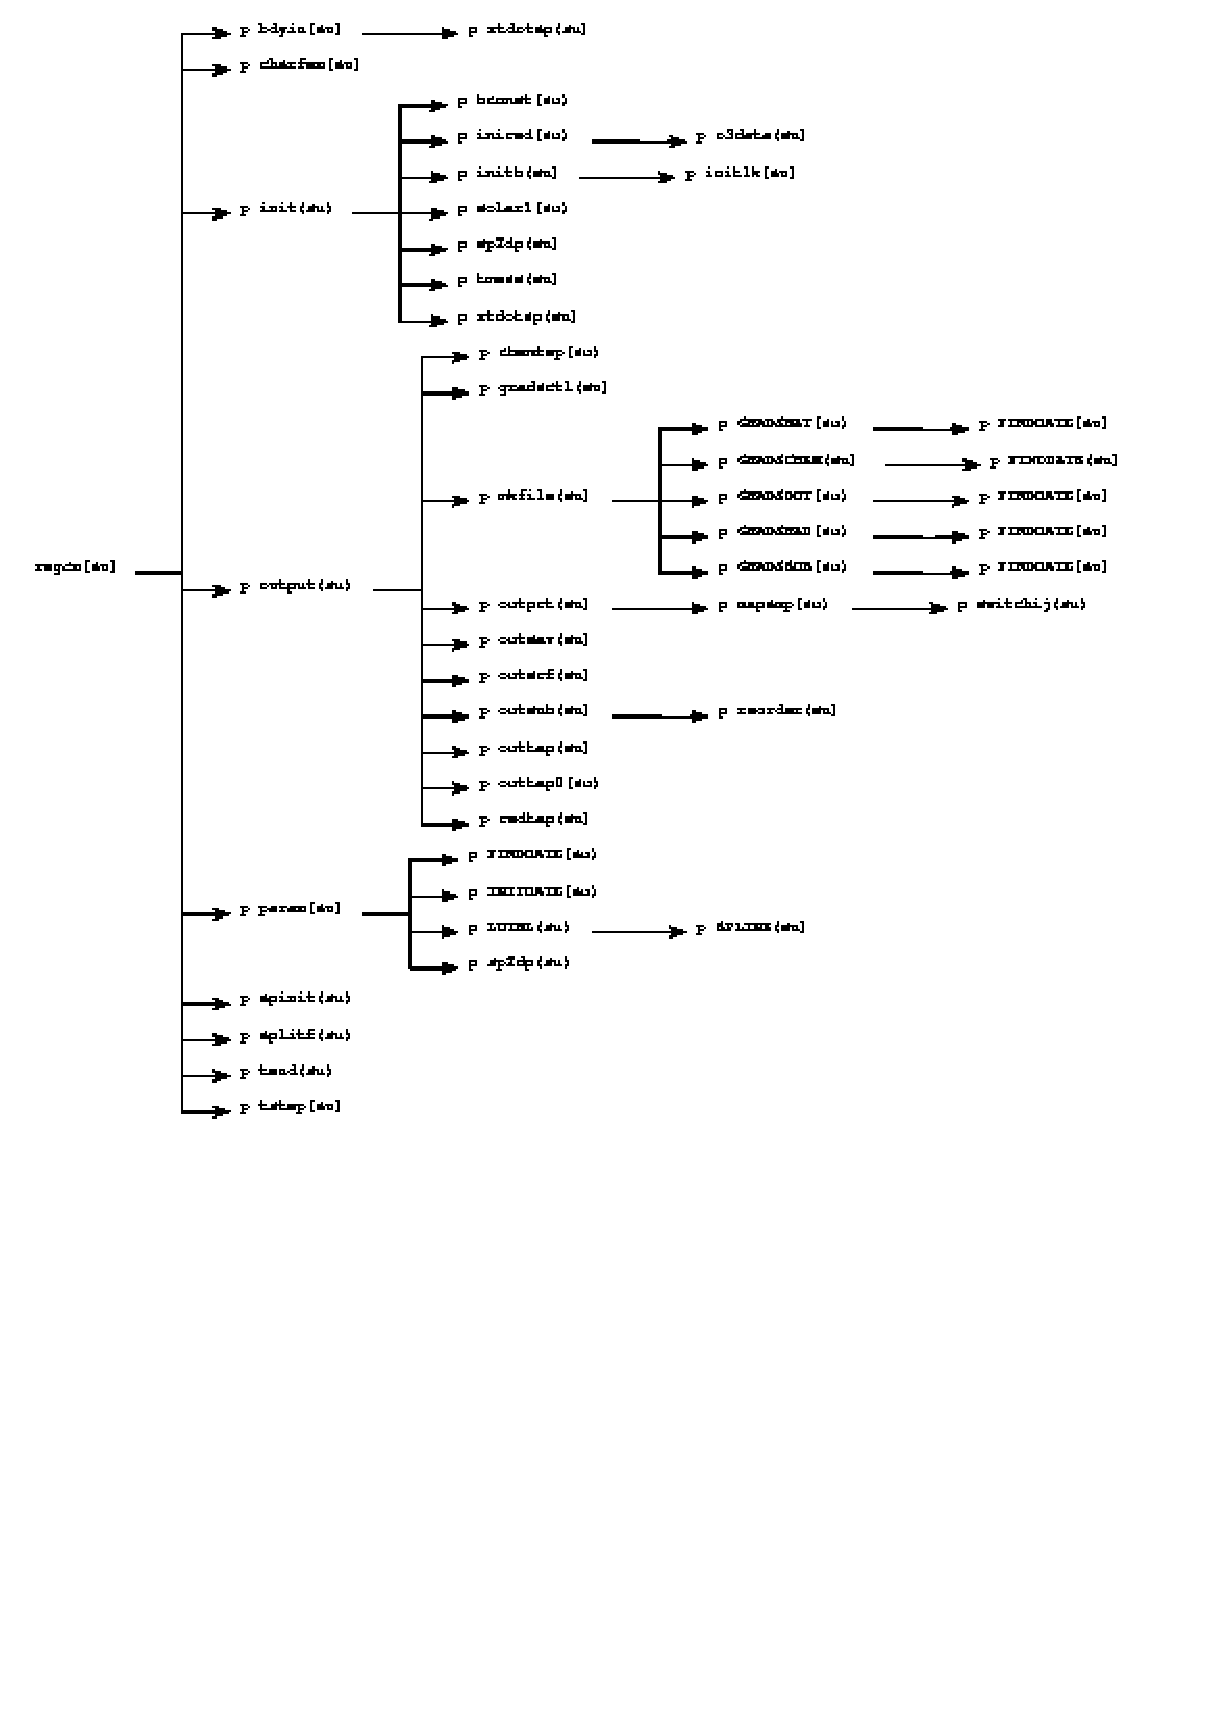
\includegraphics{xref1.fixed.eps}}
%\hspace{-1cm}
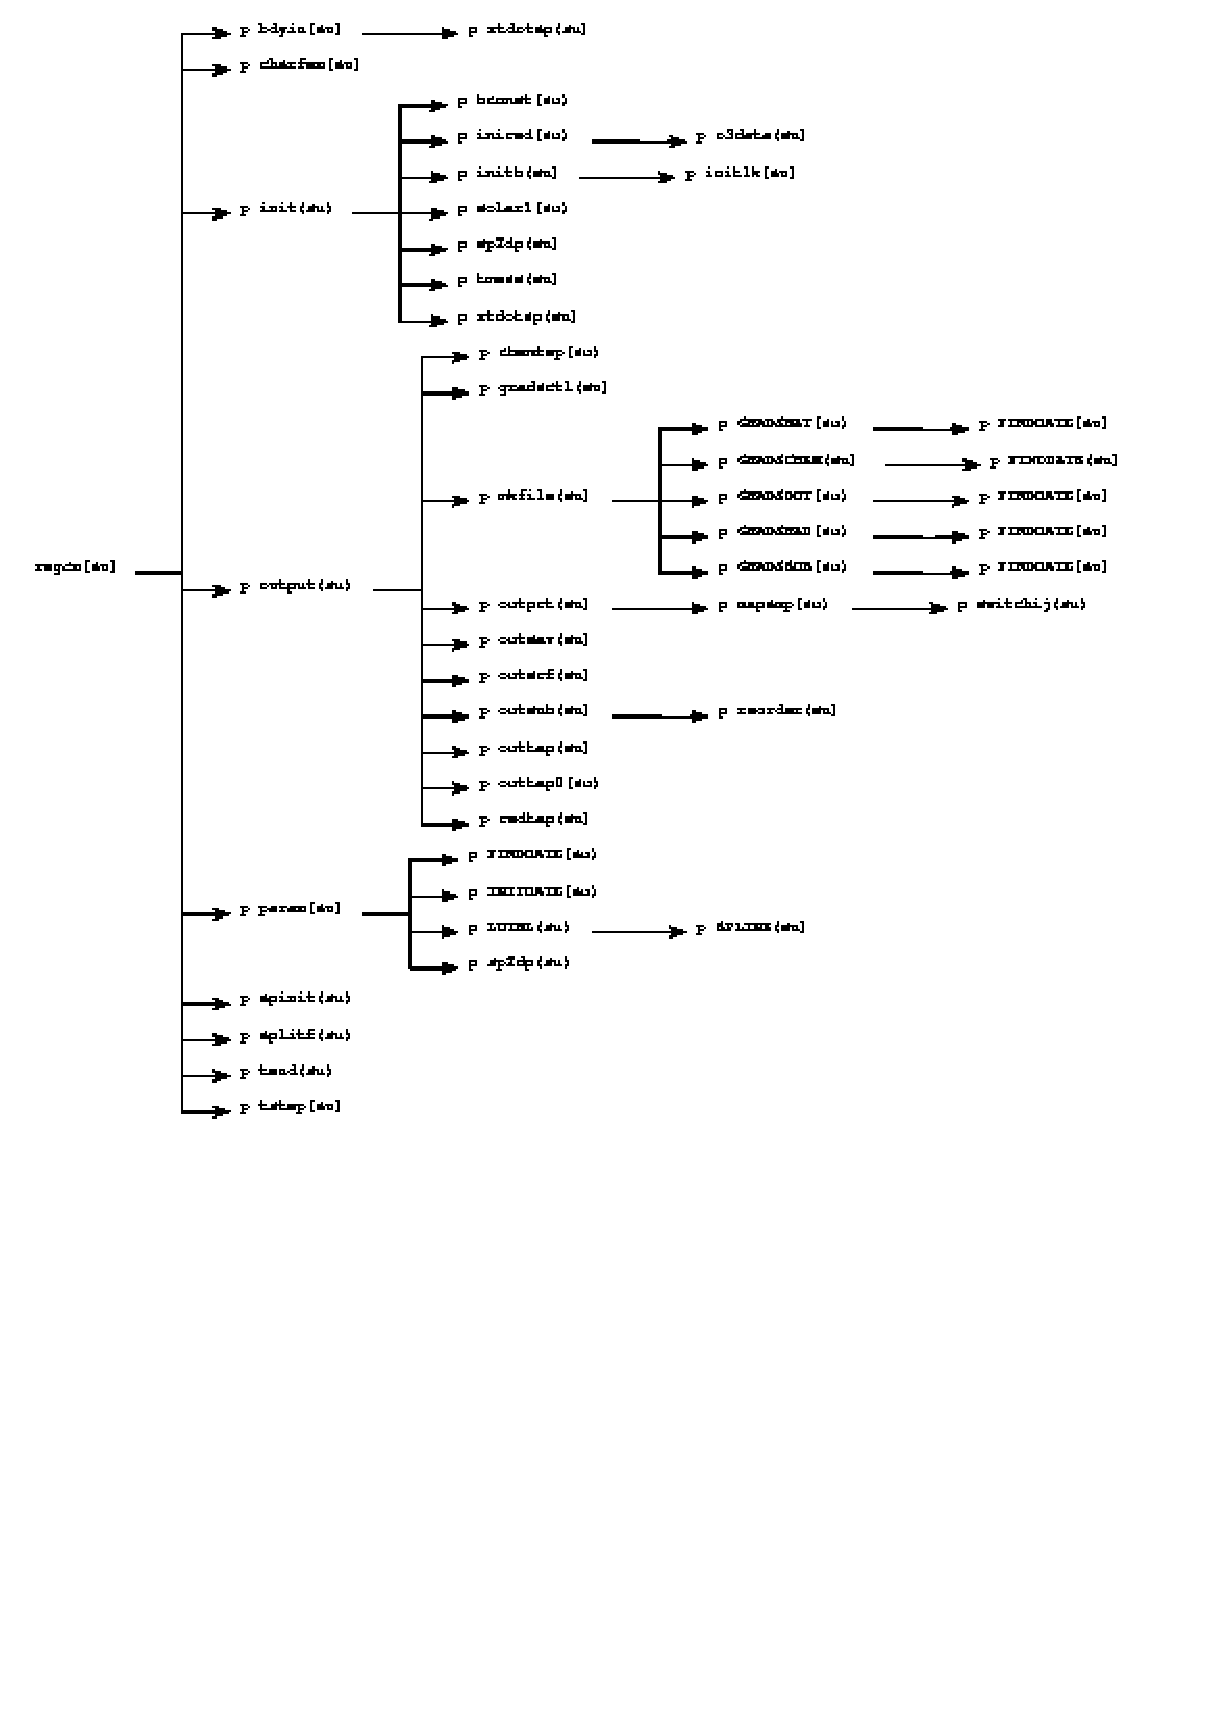
\includegraphics{xref1.fixed.eps}
\end{center}
\caption{flow chart of }  \label{grid}
\end{figure}

\begin{figure}
\begin{center}
%\resizebox{6.0in}{!}{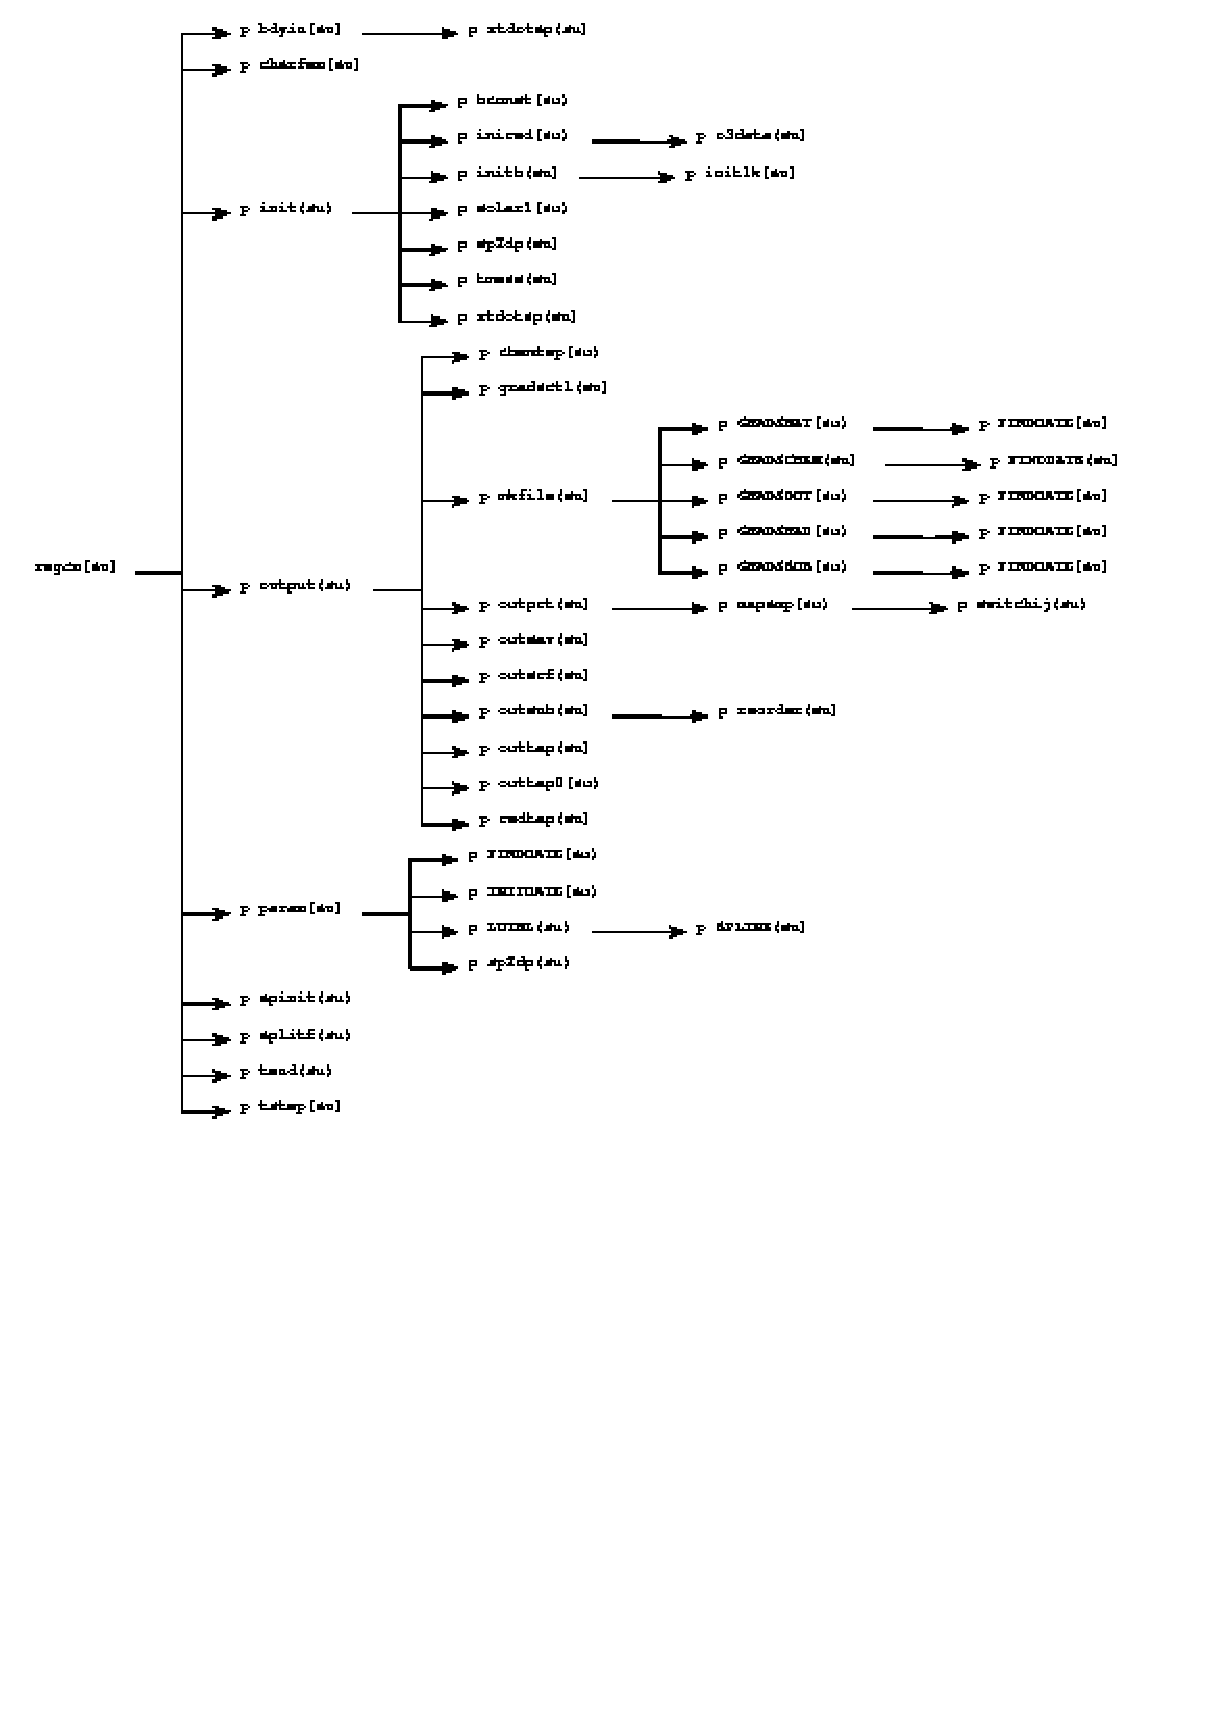
\includegraphics{xref1.fixed.eps}}
\hspace{-1cm}
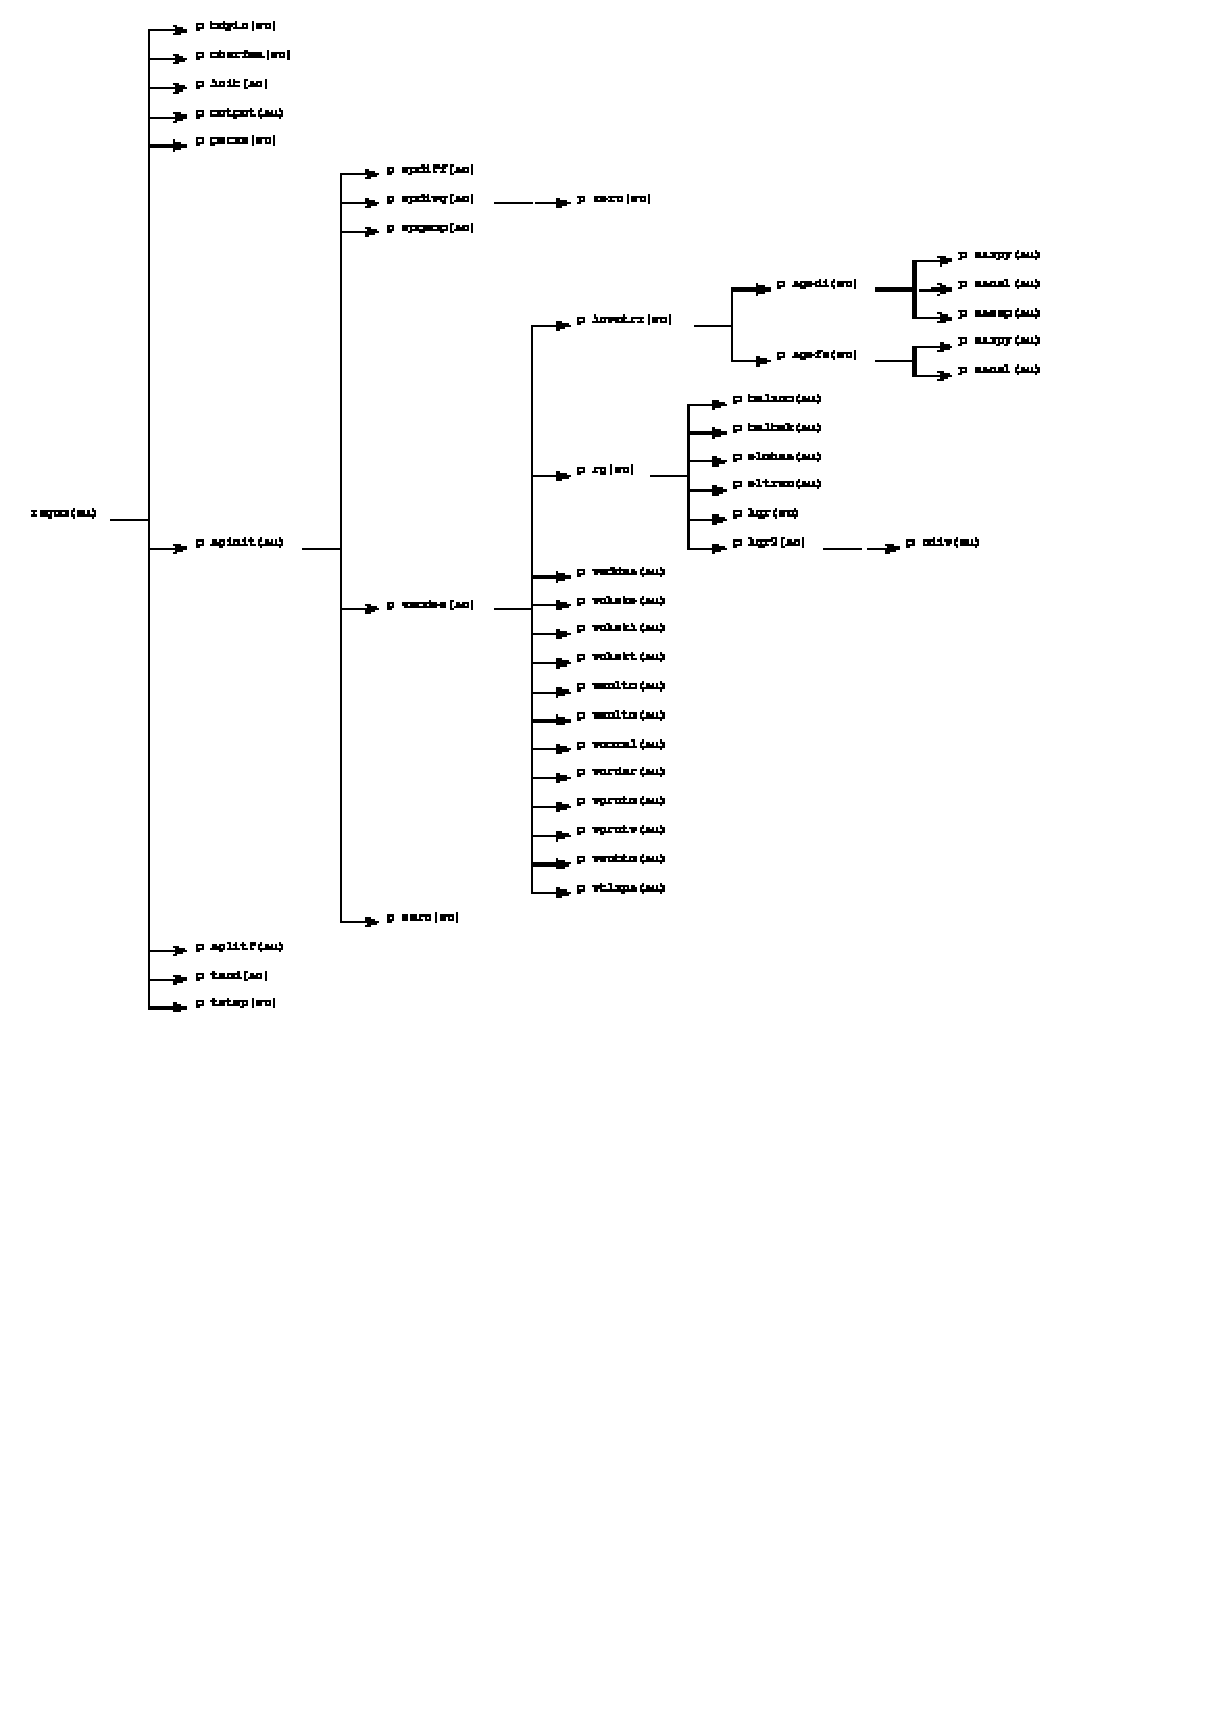
\includegraphics{xref2.fixed.eps}
\caption{xref1}  \label{grid}
\end{center}
\end{figure}

\begin{figure}
\begin{center}
%\resizebox{6.0in}{!}{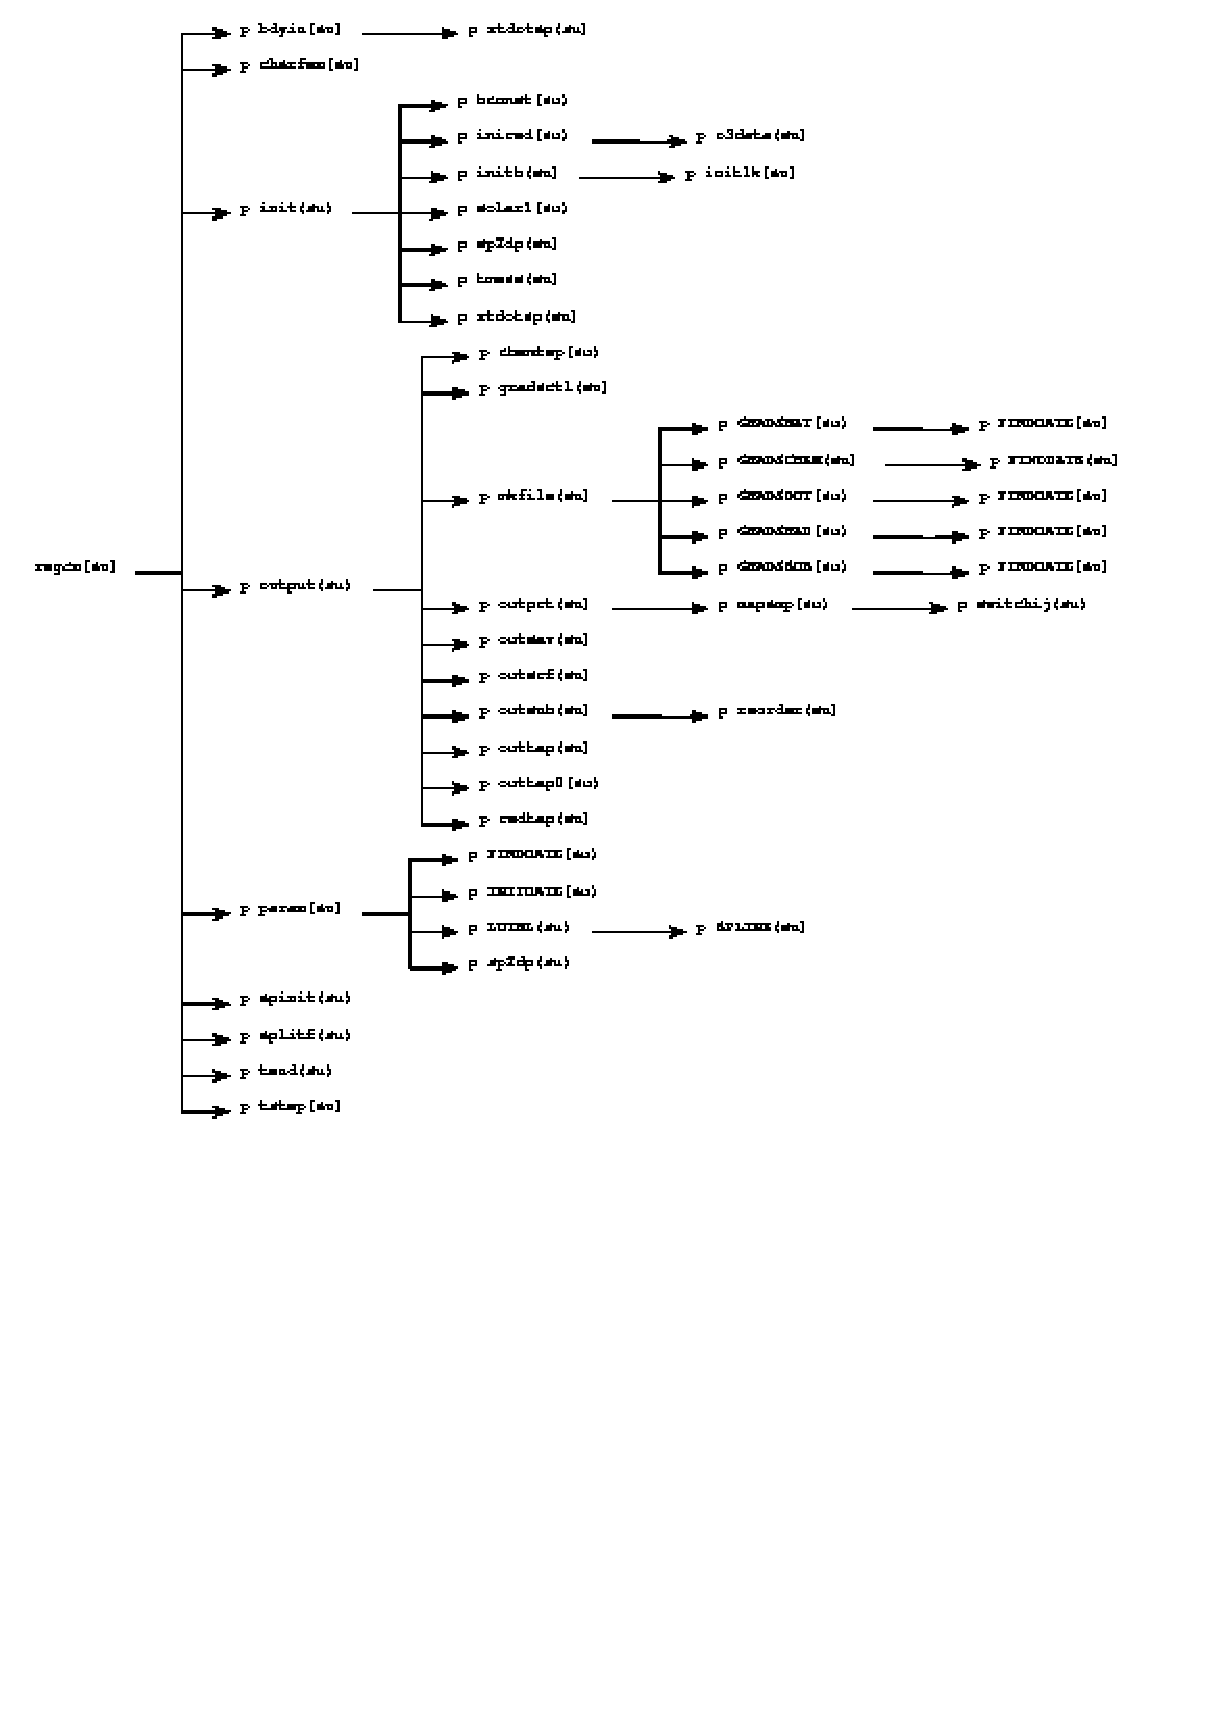
\includegraphics{xref1.fixed.eps}}
\hspace{-1cm}
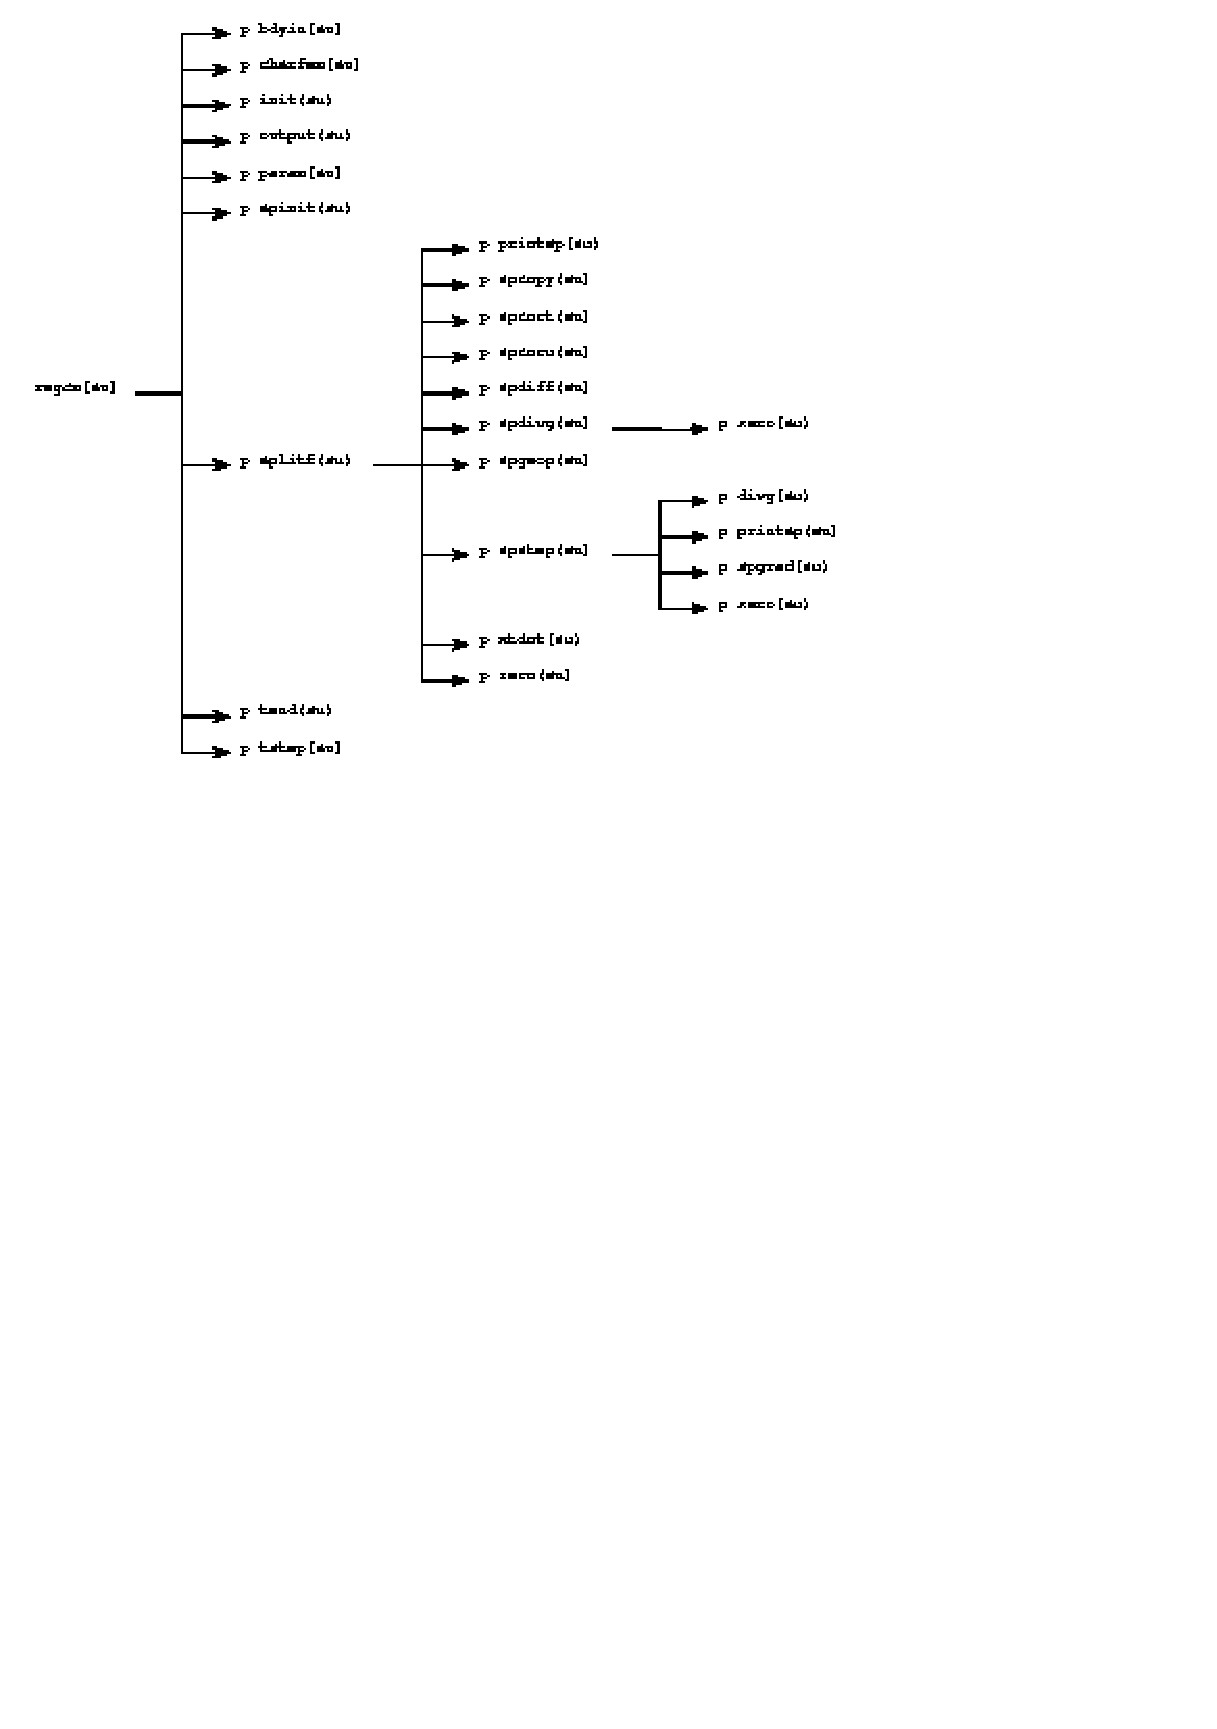
\includegraphics{xref3.fixed.eps}
\caption{xref1}  \label{grid}
\end{center}
\end{figure}

\begin{figure}
\begin{center}
%\resizebox{6.0in}{!}{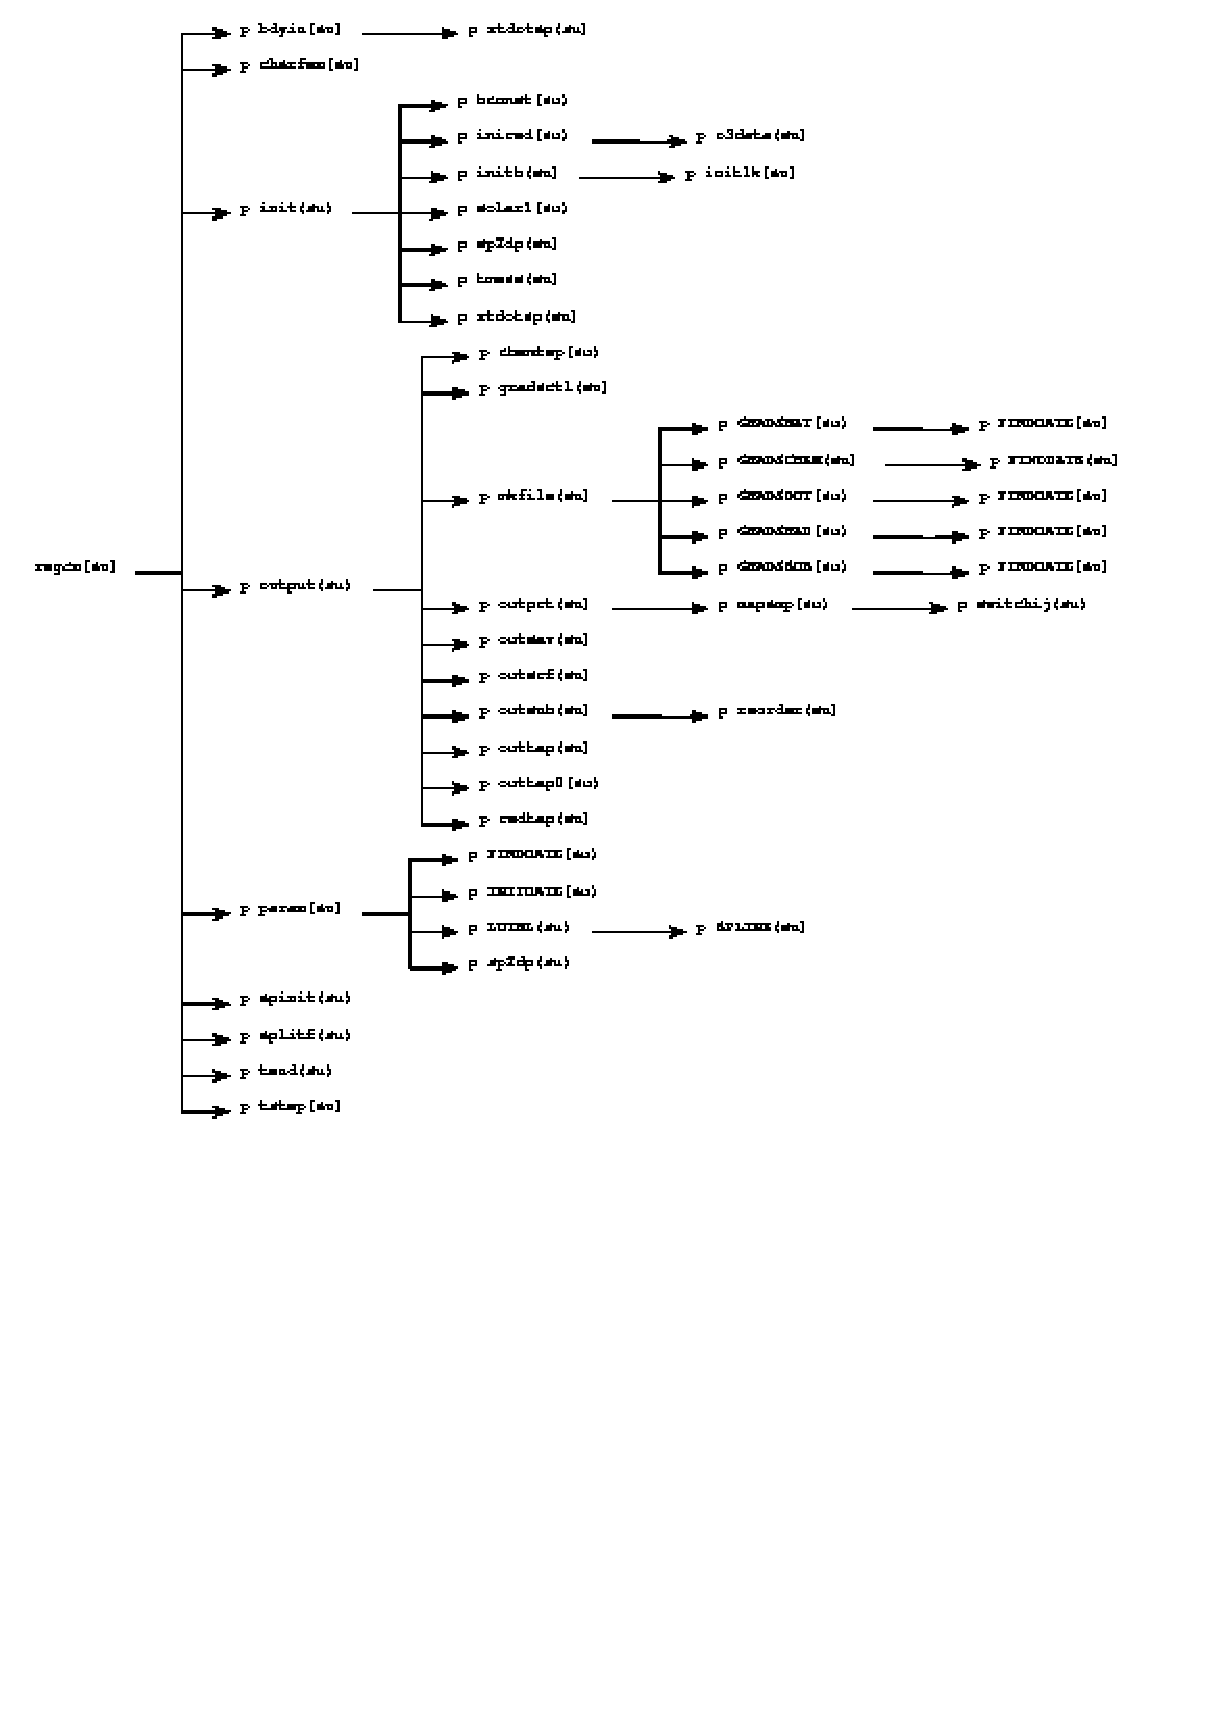
\includegraphics{xref1.fixed.eps}}
\hspace{-1cm}
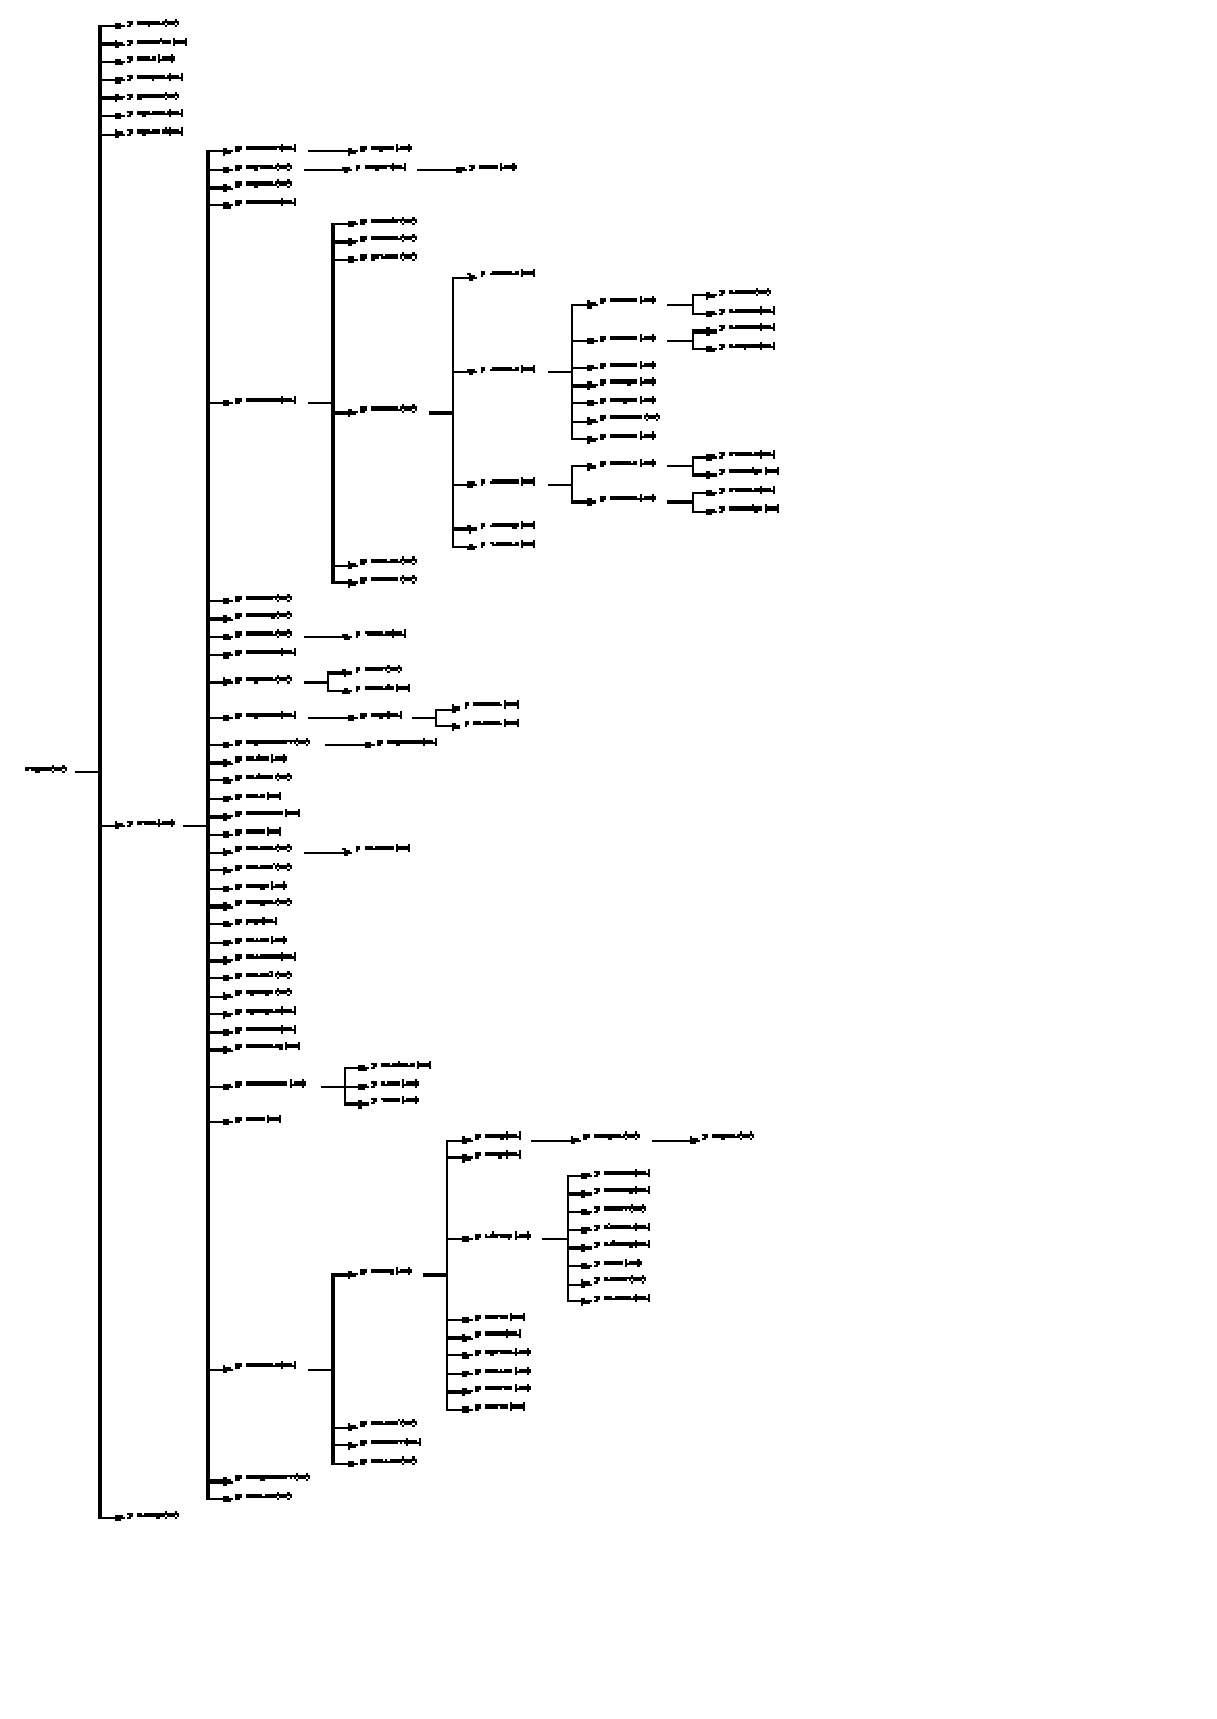
\includegraphics{xref4.fixed.eps}
\end{center}
\caption{xref1}  \label{grid}
\end{figure}




%\include{figures}

\end{document}
